\documentclass[10pt]{article}
\usepackage[a4paper,margin=1.8cm]{geometry}
\usepackage[utf8]{inputenc}
\usepackage[T1]{fontenc}
\usepackage{lmodern,amsmath,booktabs,longtable,makecell,pdfpages,array}
\usepackage[hidelinks]{hyperref}
\DeclareUnicodeCharacter{2212}{\ensuremath{-}}
\DeclareUnicodeCharacter{03B1}{\ensuremath{\alpha}}
\DeclareUnicodeCharacter{03BA}{\ensuremath{\kappa}}
\DeclareUnicodeCharacter{0394}{\ensuremath{\Delta}}
\DeclareUnicodeCharacter{2265}{\ensuremath{\geq}}
\DeclareUnicodeCharacter{2264}{\ensuremath{\leq}}
\DeclareUnicodeCharacter{2192}{\ensuremath{\rightarrow}}
\DeclareUnicodeCharacter{00D7}{\ensuremath{\times}}
\renewcommand{\thetable}{S\arabic{table}}
\setlength{\LTcapwidth}{\textwidth}
\title{Supplementary material\\[4pt]\large False-Alarm Calibration Transport Across Engines in Full-Flight Aero-Engine
Anomaly Detection: A Multi-Subset Audit of Context Conditioning and Calibration-Fleet Coverage}
\author{Jinghang Mei}
\date{}
\begin{document}
\maketitle

\section*{Part A. Multi-subset extension}
\noindent\textbf{Contents.} Part A reports the frozen multi-subset extension (Sections 3--4 of the article): cohort
eligibility, engine roles, locks and numerical checks, every detector run's phase FPRs and transport metrics, per-engine
errors, bootstrap intervals, target sensitivity, calibration-fleet composition, alarm persistence, matched-burden delay,
abnormal-state alarm rates, the reference reproduction gates, the post hoc checks of Section 4.9 and the final focused validation of Section 4.8. Part B reproduces, unchanged, the supplement of the
pre-extension study: the frozen DS02 discovery and one-shot DS03 confirmation, the post-confirmation analyses and the
adversarial validation, which Section 4.1 of the article summarizes.

\noindent\textbf{Conventions.} FPRs are healthy ($hs = 1$) row-level false-positive rates; pp = percentage points. Runs:
PCA (one run), Isolation Forest (IF), past-only LSTM and CVAE (seeds s0--s2). Arms: P pooled; C retrospective
phase-conditioned (uses complete-flight phases); Q continuous-context quantile regression (adversarial control). Families:
F1 = DS01, F2 = DS04, F3 = DS05--DS07, F4 = DS08a, F5 = DS08c; DS02 and DS03 are references and decide no hypothesis.
Machine-readable values: results/extension/ and paper/mssp\_extended/evidence/ (with SHA-256 sums); every number in the
article is traced in docs/extension/EXTENSION\_EVIDENCE\_LEDGER.csv.

\noindent\textbf{Amendments} (docs/extension/AMENDMENTS.md; each preceded every affected outcome). (1) Two classification
rules (original-story class and H2 verdict) were completed so that every outcome configuration has a class; no threshold
changed. (2) After a stop rule fired on a non-finite CVAE training loss (DS01), the encoder log-variance was bounded and
gradients were clipped at norm 1.0 for every subset and seed; the DS01 lock was rerun from scratch. (3) Healthy and
post-onset audit rows are scored in separate calls, as in the frozen stages, after the first DS03 reference attempt failed a
reproduction gate at float32 rounding level; the reference work was rerun and passed before any new-subset audit.

\clearpage
\subsection*{A.1 Cohort, roles, locks and training}
{\footnotesize
\setlength{\tabcolsep}{3.5pt}
\begin{longtable}{llp{3.2cm}p{2.6cm}rrrl}
\caption{Candidate subsets, metadata-only eligibility audit (C1--C9 of the subset selection lock; y = pass, n = fail). DS02 and DS03 fail C9 by construction (opened by the frozen study) and are references. DS08d fails C1 (the official file is 32 bytes shorter than its HDF5 superblock declares) and was not opened.}\label{tab:cohort}\\
\toprule
\makecell[b]{Subset} & \makecell[b]{Role} & \makecell[b]{Dev engines\\(unit:class)} & \makecell[b]{Test engines\\(unit:class)} & \makecell[b]{Healthy flights\\dev / test} & \makecell[b]{Post-onset\\flights (test)} & \makecell[b]{Min. test engine\\rows per phase} & \makecell[b]{C1--C9} \\
\midrule
\endfirsthead
\toprule
\makecell[b]{Subset} & \makecell[b]{Role} & \makecell[b]{Dev engines\\(unit:class)} & \makecell[b]{Test engines\\(unit:class)} & \makecell[b]{Healthy flights\\dev / test} & \makecell[b]{Post-onset\\flights (test)} & \makecell[b]{Min. test engine\\rows per phase} & \makecell[b]{C1--C9} \\
\midrule
\endhead
\bottomrule
\endfoot
DS01 & primary cohort & 1:1 2:3 3:2 4:1 5:3 6:2 & 7:1 8:2 9:1 10:3 & 158 / 111 & 230 & 31,432 & yyyyyyyyy \\
DS02 & REFERENCE & 2:3 5:3 10:3 16:3 18:3 20:3 & 11:3 14:1 15:2 & 95 / 76 & 126 & 12,241 & yyyyyyyyn \\
DS03 & REFERENCE & 1:1 2:2 3:2 4:2 5:1 6:3 7:2 8:3 9:1 & 10:3 11:3 12:1 13:3 14:1 15:2 & 237 / 148 & 290 & 33,331 & yyyyyyyyn \\
DS04 & primary cohort & 1:2 2:3 3:2 4:3 5:3 6:3 & 7:2 8:2 9:2 10:3 & 105 / 79 & 265 & 47,345 & yyyyyyyyy \\
DS05 & primary cohort & 1:2 2:3 3:2 4:1 5:1 6:3 & 7:2 8:1 9:3 10:1 & 153 / 112 & 215 & 33,438 & yyyyyyyyy \\
DS06 & primary cohort & 1:2 2:3 3:2 4:1 5:1 6:3 & 7:2 8:1 9:3 10:1 & 141 / 100 & 222 & 29,592 & yyyyyyyyy \\
DS07 & primary cohort & 1:2 2:3 3:2 4:1 5:1 6:3 & 7:2 8:1 9:3 10:1 & 154 / 113 & 231 & 34,148 & yyyyyyyyy \\
DS08a & primary cohort & 1:1 2:3 3:1 4:2 5:2 6:3 7:2 8:2 9:1 & 10:1 11:2 12:3 13:3 14:3 15:1 & 197 / 122 & 261 & 24,255 & yyyyyyyyy \\
DS08c & primary cohort & 1:3 2:3 3:3 4:3 5:3 6:2 & 7:2 8:2 9:2 10:2 & 100 / 86 & 151 & 48,940 & yyyyyyyyy \\
DS08d & EXCLUDED & -- & -- & -- & -- & -- & C1 fails; not opened \\
\end{longtable}
\vspace{-0.6em}
\noindent{\scriptsize Source: docs/extension/subset\_metadata\_audit.csv (labels, variable names and healthy-row altitude only).}
}

{\footnotesize
\setlength{\tabcolsep}{3.5pt}
\begin{longtable}{llp{2.7cm}lp{2.6cm}p{3.4cm}l}
\caption{Engine roles (R-ALLOC for new subsets; frozen roles for DS02 and DS03).}\label{tab:roles}\\
\toprule
\makecell[b]{Subset} & \makecell[b]{Family} & \makecell[b]{Fit (class)} & \makecell[b]{Validation} & \makecell[b]{Calibration (class)} & \makecell[b]{Audit (class)} & \makecell[b]{Composition N} \\
\midrule
\endfirsthead
\toprule
\makecell[b]{Subset} & \makecell[b]{Family} & \makecell[b]{Fit (class)} & \makecell[b]{Validation} & \makecell[b]{Calibration (class)} & \makecell[b]{Audit (class)} & \makecell[b]{Composition N} \\
\midrule
\endhead
\bottomrule
\endfoot
DS02 & ref. & 2 (3), 5 (3), 10 (3), 16 (3) & 16 & 18 (3), 20 (3) & 11 (3), 14 (1), 15 (2) & not eligible \\
DS03 & ref. & 1 (1), 2 (2), 3 (2), 5 (1), 6 (3), 7 (2), 9 (1) & 9 & 4 (2), 8 (3) & 10 (3), 11 (3), 12 (1), 13 (3), 14 (1), 15 (2) & 102,000 \\
DS01 & F1 & 1 (1), 2 (3), 3 (2) & 3 & 4 (1), 5 (3), 6 (2) & 7 (1), 8 (2), 9 (1), 10 (3) & 78,000 \\
DS04 & F2 & 1 (2), 2 (3), 4 (3) & 4 & 3 (2), 5 (3), 6 (3) & 7 (2), 8 (2), 9 (2), 10 (3) & 96,000 \\
DS05 & F3 & 1 (2), 2 (3), 4 (1) & 4 & 3 (2), 5 (1), 6 (3) & 7 (2), 8 (1), 9 (3), 10 (1) & 78,000 \\
DS06 & F3 & 1 (2), 2 (3), 4 (1) & 4 & 3 (2), 5 (1), 6 (3) & 7 (2), 8 (1), 9 (3), 10 (1) & 66,000 \\
DS07 & F3 & 1 (2), 2 (3), 4 (1) & 4 & 3 (2), 5 (1), 6 (3) & 7 (2), 8 (1), 9 (3), 10 (1) & 78,000 \\
DS08a & F4 & 1 (1), 2 (3), 4 (2) & 4 & 3 (1), 5 (2), 6 (3), 7 (2), 8 (2), 9 (1) & 10 (1), 11 (2), 12 (3), 13 (3), 14 (3), 15 (1) & 60,000 \\
DS08c & F5 & 1 (3), 2 (3), 6 (2) & 6 & 3 (3), 4 (3), 5 (3) & 7 (2), 8 (2), 9 (2), 10 (2) & not eligible \\
\end{longtable}
\vspace{-0.6em}
\noindent{\scriptsize Source: results/extension/$\langle$subset$\rangle$/lock/calibration\_lock.json.}
}

{\footnotesize
\setlength{\tabcolsep}{3.5pt}
\begin{longtable}{lrrrrrrr}
\caption{Calibration locks, compute and CVAE numerical checks. The float64 check rescored calibration rows in double precision; the variance-bound share is the fraction of decoder outputs within 1\% of the lower log-variance bound. For the references DS02 and DS03 the audit time is the whole reference rerun (CVAE training, lock and audit; the frozen residual models are refitted or loaded).}\label{tab:locks}\\
\toprule
\makecell[b]{Subset} & \makecell[b]{Calibration\\rows / flights} & \makecell[b]{Lock (s)} & \makecell[b]{Audit (s)} & \makecell[b]{Audit rows} & \makecell[b]{CVAE float64 check:\\min Spearman} & \makecell[b]{CVAE exceedance\\changes} & \makecell[b]{CVAE variance-bound share\\(seeds 0/1/2)} \\
\midrule
\endfirsthead
\toprule
\makecell[b]{Subset} & \makecell[b]{Calibration\\rows / flights} & \makecell[b]{Lock (s)} & \makecell[b]{Audit (s)} & \makecell[b]{Audit rows} & \makecell[b]{CVAE float64 check:\\min Spearman} & \makecell[b]{CVAE exceedance\\changes} & \makecell[b]{CVAE variance-bound share\\(seeds 0/1/2)} \\
\midrule
\endhead
\bottomrule
\endfoot
DS01 & 648,562 / 79 & 3,732 & 126 & 2,735,232 & 1.000000 & 0 & 73.5\% / 42.0\% / 25.5\% \\
DS04 & 649,001 / 53 & 4,627 & 169 & 3,602,561 & 1.000000 & 0 & 0.1\% / 11.4\% / 26.0\% \\
DS05 & 600,857 / 77 & 3,336 & 113 & 2,562,046 & 1.000000 & 2 & 67.5\% / 1.7\% / 46.7\% \\
DS06 & 559,506 / 71 & 3,029 & 116 & 2,522,447 & 1.000000 & 2 & 0.0\% / 31.8\% / 37.2\% \\
DS07 & 612,770 / 78 & 3,681 & 126 & 2,869,786 & 1.000000 & 1 & 0.7\% / 19.4\% / 11.9\% \\
DS08a & 984,555 / 131 & 10,496 & 196 & 3,722,997 & 1.000000 & 2 & 0.0\% / 1.7\% / 30.6\% \\
DS08c & 692,465 / 47 & 4,766 & 118 & 2,117,819 & 1.000000 & 1 & 16.0\% / 0.2\% / 0.2\% \\
DS02 & 386,643 / 32 & -- & 2,215 & 1,253,743 & 1.000000 & 2 & 45.5\% / 11.9\% / 0.0\% \\
DS03 & 458,105 / 40 & -- & 3,266 & 4,251,560 & 1.000000 & 0 & 88.2\% / 84.1\% / 9.6\% \\
\end{longtable}
\vspace{-0.6em}
\noindent{\scriptsize Source: results/extension/summary/numerical\_audit\_locks.csv.}
}

{\footnotesize
\setlength{\tabcolsep}{3.5pt}
\begin{longtable}{llrrlrrrl}
\caption{Epoch selection and refit of the LSTM and CVAE (selection on the validation engine, refit on the full fit pool). DS02/DS03 LSTM checkpoints are frozen and not retrained.}\label{tab:training}\\
\toprule
\makecell[b]{Subset} & \makecell[b]{Detector} & \makecell[b]{Selection\\epochs run} & \makecell[b]{Selected\\epoch} & \makecell[b]{Hit 600} & \makecell[b]{Best validation\\loss} & \makecell[b]{Refit\\epochs} & \makecell[b]{Refit final\\loss} & \makecell[b]{Refit\\finite} \\
\midrule
\endfirsthead
\toprule
\makecell[b]{Subset} & \makecell[b]{Detector} & \makecell[b]{Selection\\epochs run} & \makecell[b]{Selected\\epoch} & \makecell[b]{Hit 600} & \makecell[b]{Best validation\\loss} & \makecell[b]{Refit\\epochs} & \makecell[b]{Refit final\\loss} & \makecell[b]{Refit\\finite} \\
\midrule
\endhead
\bottomrule
\endfoot
DS01 & CVAE s0 & 81 & 75 & no & -30.16 & 75 & -44.62 & yes \\
DS01 & CVAE s1 & 58 & 52 & no & -32.12 & 52 & -39.84 & yes \\
DS01 & CVAE s2 & 42 & 36 & no & -36.99 & 36 & -36.66 & yes \\
DS01 & LSTM s0 & 180 & 174 & no & 138.2 & 174 & 0.05613 & yes \\
DS01 & LSTM s1 & 130 & 124 & no & 138.2 & 124 & 0.07002 & yes \\
DS01 & LSTM s2 & 150 & 144 & no & 138.2 & 144 & 0.06771 & yes \\
\midrule
DS04 & CVAE s0 & 22 & 16 & no & -34.07 & 16 & -20.23 & yes \\
DS04 & CVAE s1 & 35 & 29 & no & -37.4 & 29 & -34.24 & yes \\
DS04 & CVAE s2 & 39 & 33 & no & -36.36 & 33 & -34.3 & yes \\
DS04 & LSTM s0 & 598 & 592 & no & 0.1726 & 592 & 0.1658 & yes \\
DS04 & LSTM s1 & 584 & 582 & no & 0.1699 & 582 & 0.1618 & yes \\
DS04 & LSTM s2 & 352 & 349 & no & 0.1876 & 349 & 0.1808 & yes \\
\midrule
DS05 & CVAE s0 & 72 & 66 & no & -40.8 & 66 & -41.89 & yes \\
DS05 & CVAE s1 & 24 & 18 & no & -30.79 & 18 & -26.11 & yes \\
DS05 & CVAE s2 & 55 & 49 & no & -40.14 & 49 & -39.41 & yes \\
DS05 & LSTM s0 & 370 & 369 & no & 0.07237 & 369 & 0.03416 & yes \\
DS05 & LSTM s1 & 341 & 337 & no & 0.07487 & 337 & 0.03637 & yes \\
DS05 & LSTM s2 & 414 & 411 & no & 0.06801 & 411 & 0.03142 & yes \\
\midrule
DS06 & CVAE s0 & 20 & 14 & no & -27.3 & 14 & -19.74 & yes \\
DS06 & CVAE s1 & 45 & 39 & no & -36.21 & 39 & -38.38 & yes \\
DS06 & CVAE s2 & 46 & 40 & no & -35.35 & 40 & -40.64 & yes \\
DS06 & LSTM s0 & 473 & 468 & no & 0.07893 & 468 & 0.03078 & yes \\
DS06 & LSTM s1 & 510 & 508 & no & 0.07897 & 508 & 0.02874 & yes \\
DS06 & LSTM s2 & 447 & 446 & no & 0.07853 & 446 & 0.03265 & yes \\
\midrule
DS07 & CVAE s0 & 41 & 35 & no & -35.43 & 35 & -35.39 & yes \\
DS07 & CVAE s1 & 39 & 33 & no & -35.87 & 33 & -38.18 & yes \\
DS07 & CVAE s2 & 29 & 23 & no & -33.78 & 23 & -34.66 & yes \\
DS07 & LSTM s0 & 365 & 365 & no & 0.09256 & 365 & 0.03516 & yes \\
DS07 & LSTM s1 & 355 & 352 & no & 0.08867 & 352 & 0.0365 & yes \\
DS07 & LSTM s2 & 417 & 417 & no & 0.0843 & 417 & 0.03184 & yes \\
\midrule
DS08a & CVAE s0 & 33 & 27 & no & -35.72 & 27 & -35.55 & yes \\
DS08a & CVAE s1 & 30 & 24 & no & -34.36 & 24 & -34.85 & yes \\
DS08a & CVAE s2 & 52 & 46 & no & -39.7 & 46 & -38.66 & yes \\
DS08a & LSTM s0 & 535 & 532 & no & 0.0911 & 532 & 0.02193 & yes \\
DS08a & LSTM s1 & 380 & 374 & no & 0.1369 & 374 & 0.0317 & yes \\
DS08a & LSTM s2 & 321 & 315 & no & 0.1571 & 315 & 0.03802 & yes \\
\midrule
DS08c & CVAE s0 & 36 & 30 & no & -29.71 & 30 & -30.66 & yes \\
DS08c & CVAE s1 & 24 & 18 & no & -7.642 & 18 & -18.64 & yes \\
DS08c & CVAE s2 & 21 & 15 & no & -16.24 & 15 & -26.25 & yes \\
DS08c & LSTM s0 & 257 & 251 & no & 233.6 & 251 & 0.03831 & yes \\
DS08c & LSTM s1 & 134 & 128 & no & 233.8 & 128 & 0.06229 & yes \\
DS08c & LSTM s2 & 210 & 204 & no & 233.7 & 204 & 0.04536 & yes \\
\midrule
DS02 & CVAE s0 & 35 & 29 & no & -40.65 & 29 & -40.27 & yes \\
DS02 & CVAE s1 & 24 & 18 & no & -36.17 & 18 & -38.54 & yes \\
DS02 & CVAE s2 & 16 & 10 & no & -35.22 & 10 & -32.37 & yes \\
\midrule
DS03 & CVAE s0 & 60 & 54 & no & -46.75 & 54 & -47.02 & yes \\
DS03 & CVAE s1 & 48 & 42 & no & -46.79 & 42 & -45.89 & yes \\
DS03 & CVAE s2 & 21 & 15 & no & -41.88 & 15 & -38.66 & yes \\
\end{longtable}
\vspace{-0.6em}
\noindent{\scriptsize Source: results/extension/summary/numerical\_audit\_training.csv. Losses are per-row negative log-likelihoods (CVAE) or mean squared errors (LSTM) on the standardized scale.}
}

\clearpage
\subsection*{A.2 Calibration transport (1\% target)}
{\footnotesize
\setlength{\tabcolsep}{3.5pt}
\begin{longtable}{lllrrrrrrrrr}
\caption{Row-pooled phase FPRs and transport metrics for every subset, detector run and arm at the 1\% target (P pooled, C retrospective phase-conditioned, Q continuous context).}\label{tab:transport}\\
\toprule
\makecell[b]{Subset} & \makecell[b]{Run} & \makecell[b]{Arm} & \makecell[b]{Climb\\FPR (\%)} & \makecell[b]{Cruise\\FPR (\%)} & \makecell[b]{Descent\\FPR (\%)} & \makecell[b]{Pooled\\A1 (pp)} & \makecell[b]{Pooled\\A2 (pp)} & \makecell[b]{ME-A2\\(pp)} & \makecell[b]{WE-A2\\(pp)} & \makecell[b]{EW-A2\\(pp)} & \makecell[b]{Worst\\engine} \\
\midrule
\endfirsthead
\toprule
\makecell[b]{Subset} & \makecell[b]{Run} & \makecell[b]{Arm} & \makecell[b]{Climb\\FPR (\%)} & \makecell[b]{Cruise\\FPR (\%)} & \makecell[b]{Descent\\FPR (\%)} & \makecell[b]{Pooled\\A1 (pp)} & \makecell[b]{Pooled\\A2 (pp)} & \makecell[b]{ME-A2\\(pp)} & \makecell[b]{WE-A2\\(pp)} & \makecell[b]{EW-A2\\(pp)} & \makecell[b]{Worst\\engine} \\
\midrule
\endhead
\bottomrule
\endfoot
DS02 & PCA & P & 0.12 & 0.43 & 3.46 & 3.33 & 2.46 & 2.81 & 3.97 & 2.81 & 14 \\
DS02 & PCA & C & 1.40 & 1.33 & 1.08 & 0.32 & 0.40 & 1.66 & 4.31 & 1.40 & 14 \\
DS02 & PCA & Q & 0.70 & 2.12 & 1.27 & 1.42 & 1.12 & 1.60 & 2.20 & 0.91 & 14 \\
DS02 & IF s0 & P & 0.29 & 0.57 & 2.34 & 2.05 & 1.34 & 1.38 & 1.51 & 1.38 & 14 \\
DS02 & IF s0 & C & 1.65 & 1.85 & 0.92 & 0.92 & 0.85 & 2.31 & 6.42 & 2.12 & 14 \\
DS02 & IF s0 & Q & 0.49 & 2.24 & 2.14 & 1.75 & 1.24 & 2.41 & 3.63 & 1.48 & 15 \\
DS02 & IF s1 & P & 0.25 & 0.53 & 2.67 & 2.42 & 1.67 & 1.82 & 2.29 & 1.82 & 14 \\
DS02 & IF s1 & C & 1.54 & 1.53 & 0.98 & 0.57 & 0.54 & 2.19 & 5.96 & 1.93 & 14 \\
DS02 & IF s1 & Q & 0.42 & 1.34 & 1.94 & 1.52 & 0.94 & 1.31 & 1.58 & 0.95 & 14 \\
DS02 & IF s2 & P & 0.27 & 0.58 & 2.46 & 2.19 & 1.46 & 1.52 & 1.72 & 1.52 & 14 \\
DS02 & IF s2 & C & 1.69 & 1.71 & 0.93 & 0.79 & 0.71 & 2.37 & 6.59 & 2.19 & 14 \\
DS02 & IF s2 & Q & 0.56 & 2.46 & 2.11 & 1.89 & 1.46 & 2.52 & 4.15 & 1.69 & 15 \\
DS02 & LSTM s0 & P & 0.45 & 0.71 & 2.08 & 1.63 & 1.08 & 1.03 & 1.36 & 1.02 & 11 \\
DS02 & LSTM s0 & C & 1.39 & 1.11 & 1.08 & 0.31 & 0.39 & 1.66 & 4.42 & 1.42 & 14 \\
DS02 & LSTM s0 & Q & 0.72 & 1.55 & 1.29 & 0.83 & 0.55 & 0.84 & 1.30 & 0.71 & 14 \\
DS02 & LSTM s1 & P & 0.47 & 0.73 & 2.10 & 1.63 & 1.10 & 1.06 & 1.52 & 0.98 & 11 \\
DS02 & LSTM s1 & C & 1.24 & 1.28 & 0.96 & 0.32 & 0.28 & 1.42 & 3.74 & 1.14 & 14 \\
DS02 & LSTM s1 & Q & 0.56 & 1.29 & 0.97 & 0.73 & 0.44 & 0.54 & 0.64 & 0.33 & 15 \\
DS02 & LSTM s2 & P & 0.54 & 0.75 & 2.06 & 1.52 & 1.06 & 1.13 & 1.38 & 0.96 & 11 \\
DS02 & LSTM s2 & C & 1.46 & 1.07 & 1.00 & 0.46 & 0.46 & 1.77 & 4.65 & 1.53 & 14 \\
DS02 & LSTM s2 & Q & 0.82 & 2.71 & 3.14 & 2.32 & 2.14 & 3.28 & 4.25 & 1.96 & 11 \\
DS02 & CVAE s0 & P & 0.75 & 1.12 & 2.17 & 1.42 & 1.17 & 1.41 & 2.79 & 1.41 & 14 \\
DS02 & CVAE s0 & C & 1.97 & 1.45 & 1.42 & 0.55 & 0.97 & 2.12 & 4.65 & 1.93 & 14 \\
DS02 & CVAE s0 & Q & 0.86 & 1.73 & 1.94 & 1.08 & 0.94 & 1.68 & 2.66 & 1.16 & 14 \\
DS02 & CVAE s1 & P & 1.41 & 1.66 & 2.84 & 1.42 & 1.84 & 2.86 & 6.63 & 2.64 & 14 \\
DS02 & CVAE s1 & C & 1.90 & 2.65 & 1.74 & 0.91 & 1.65 & 2.96 & 7.37 & 2.65 & 14 \\
DS02 & CVAE s1 & Q & 1.24 & 2.05 & 2.42 & 1.18 & 1.42 & 2.39 & 4.64 & 1.88 & 14 \\
DS02 & CVAE s2 & P & 1.64 & 1.15 & 2.83 & 1.68 & 1.83 & 2.69 & 6.29 & 2.63 & 14 \\
DS02 & CVAE s2 & C & 1.55 & 2.78 & 1.95 & 1.22 & 1.78 & 3.06 & 8.35 & 2.97 & 14 \\
DS02 & CVAE s2 & Q & 1.23 & 1.84 & 1.96 & 0.73 & 0.96 & 1.81 & 3.43 & 1.35 & 14 \\
\midrule
DS03 & PCA & P & 0.88 & 0.91 & 1.98 & 1.10 & 0.98 & 1.02 & 1.45 & 0.92 & 10 \\
DS03 & PCA & C & 1.86 & 1.79 & 1.23 & 0.63 & 0.86 & 1.03 & 1.52 & 0.80 & 10 \\
DS03 & PCA & Q & 2.66 & 1.80 & 1.41 & 1.25 & 1.66 & 1.84 & 7.57 & 1.33 & 10 \\
DS03 & IF s0 & P & 0.42 & 1.09 & 2.17 & 1.75 & 1.17 & 1.21 & 2.11 & 1.11 & 10 \\
DS03 & IF s0 & C & 1.66 & 1.39 & 1.27 & 0.39 & 0.66 & 0.90 & 2.37 & 0.62 & 10 \\
DS03 & IF s0 & Q & 1.96 & 1.61 & 1.70 & 0.35 & 0.96 & 1.81 & 6.31 & 0.77 & 10 \\
DS03 & IF s1 & P & 0.40 & 1.06 & 2.13 & 1.73 & 1.13 & 1.19 & 2.16 & 1.07 & 10 \\
DS03 & IF s1 & C & 1.66 & 1.37 & 1.27 & 0.40 & 0.66 & 0.86 & 2.06 & 0.62 & 10 \\
DS03 & IF s1 & Q & 1.87 & 1.50 & 1.51 & 0.37 & 0.87 & 1.74 & 6.27 & 0.63 & 10 \\
DS03 & IF s2 & P & 0.41 & 1.16 & 2.13 & 1.72 & 1.13 & 1.20 & 2.23 & 1.07 & 10 \\
DS03 & IF s2 & C & 1.74 & 1.42 & 1.27 & 0.48 & 0.74 & 0.95 & 2.56 & 0.69 & 10 \\
DS03 & IF s2 & Q & 1.90 & 1.46 & 1.59 & 0.44 & 0.90 & 1.80 & 6.44 & 0.65 & 10 \\
DS03 & LSTM s0 & P & 0.76 & 1.80 & 2.23 & 1.47 & 1.23 & 1.22 & 2.70 & 1.14 & 10 \\
DS03 & LSTM s0 & C & 1.78 & 1.83 & 1.49 & 0.34 & 0.83 & 1.22 & 2.04 & 0.86 & 12 \\
DS03 & LSTM s0 & Q & 1.51 & 1.12 & 1.69 & 0.57 & 0.69 & 1.18 & 3.67 & 0.64 & 10 \\
DS03 & LSTM s1 & P & 0.72 & 1.89 & 2.22 & 1.50 & 1.22 & 1.22 & 2.91 & 1.13 & 10 \\
DS03 & LSTM s1 & C & 1.84 & 1.76 & 1.50 & 0.35 & 0.84 & 1.20 & 2.17 & 0.94 & 12 \\
DS03 & LSTM s1 & Q & 1.72 & 1.19 & 1.71 & 0.53 & 0.72 & 1.38 & 4.91 & 0.67 & 10 \\
DS03 & LSTM s2 & P & 0.77 & 1.98 & 2.19 & 1.42 & 1.19 & 1.30 & 3.08 & 1.09 & 10 \\
DS03 & LSTM s2 & C & 1.80 & 1.72 & 1.53 & 0.27 & 0.80 & 1.24 & 2.02 & 0.87 & 12 \\
DS03 & LSTM s2 & Q & 1.49 & 1.06 & 1.63 & 0.57 & 0.63 & 1.18 & 3.59 & 0.58 & 10 \\
DS03 & CVAE s0 & P & 0.50 & 2.71 & 1.95 & 2.22 & 1.71 & 1.87 & 3.83 & 1.19 & 10 \\
DS03 & CVAE s0 & C & 2.17 & 2.32 & 1.33 & 0.99 & 1.32 & 1.83 & 4.73 & 1.01 & 10 \\
DS03 & CVAE s0 & Q & 2.63 & 3.13 & 1.95 & 1.18 & 2.13 & 2.10 & 8.47 & 1.60 & 10 \\
DS03 & CVAE s1 & P & 0.92 & 1.18 & 1.65 & 0.74 & 0.65 & 1.03 & 1.64 & 0.55 & 11 \\
DS03 & CVAE s1 & C & 1.77 & 1.06 & 1.28 & 0.71 & 0.77 & 1.23 & 3.06 & 0.92 & 12 \\
DS03 & CVAE s1 & Q & 1.28 & 1.15 & 1.68 & 0.52 & 0.68 & 0.93 & 1.62 & 0.60 & 11 \\
DS03 & CVAE s2 & P & 0.69 & 1.17 & 2.05 & 1.37 & 1.05 & 1.00 & 1.74 & 0.99 & 11 \\
DS03 & CVAE s2 & C & 1.30 & 1.97 & 1.26 & 0.71 & 0.97 & 1.10 & 1.53 & 0.92 & 12 \\
DS03 & CVAE s2 & Q & 0.86 & 1.52 & 1.32 & 0.67 & 0.52 & 0.69 & 1.06 & 0.52 & 11 \\
\midrule
DS01 & PCA & P & 1.15 & 0.62 & 1.99 & 1.37 & 0.99 & 0.98 & 1.50 & 0.98 & 8 \\
DS01 & PCA & C & 2.08 & 1.08 & 1.16 & 0.99 & 1.08 & 1.11 & 1.31 & 1.09 & 9 \\
DS01 & PCA & Q & 2.29 & 1.76 & 1.51 & 0.78 & 1.29 & 1.28 & 2.57 & 0.98 & 8 \\
DS01 & IF s0 & P & 0.85 & 0.44 & 1.95 & 1.51 & 0.95 & 0.97 & 1.57 & 0.97 & 7 \\
DS01 & IF s0 & C & 1.18 & 1.10 & 0.97 & 0.21 & 0.18 & 0.47 & 0.96 & 0.32 & 7 \\
DS01 & IF s0 & Q & 0.82 & 0.97 & 1.14 & 0.32 & 0.18 & 0.63 & 0.73 & 0.27 & 9 \\
DS01 & IF s1 & P & 0.80 & 0.44 & 1.89 & 1.45 & 0.89 & 0.91 & 1.31 & 0.91 & 7 \\
DS01 & IF s1 & C & 1.19 & 1.17 & 0.89 & 0.30 & 0.19 & 0.43 & 0.96 & 0.31 & 7 \\
DS01 & IF s1 & Q & 0.78 & 0.98 & 1.09 & 0.32 & 0.22 & 0.63 & 0.71 & 0.32 & 9 \\
DS01 & IF s2 & P & 0.84 & 0.45 & 1.93 & 1.48 & 0.93 & 0.95 & 1.49 & 0.95 & 7 \\
DS01 & IF s2 & C & 1.19 & 0.98 & 0.91 & 0.28 & 0.19 & 0.44 & 0.98 & 0.32 & 7 \\
DS01 & IF s2 & Q & 0.83 & 0.98 & 1.10 & 0.27 & 0.17 & 0.65 & 0.70 & 0.27 & 10 \\
DS01 & LSTM s0 & P & 1.05 & 0.67 & 1.46 & 0.79 & 0.46 & 0.54 & 0.68 & 0.46 & 7 \\
DS01 & LSTM s0 & C & 1.13 & 1.38 & 0.92 & 0.46 & 0.38 & 0.53 & 0.75 & 0.38 & 7 \\
DS01 & LSTM s0 & Q & 1.05 & 1.33 & 1.37 & 0.32 & 0.37 & 0.75 & 1.16 & 0.42 & 10 \\
DS01 & LSTM s1 & P & 1.07 & 0.70 & 1.51 & 0.82 & 0.51 & 0.58 & 0.77 & 0.51 & 7 \\
DS01 & LSTM s1 & C & 1.14 & 1.38 & 0.96 & 0.43 & 0.38 & 0.52 & 0.90 & 0.41 & 7 \\
DS01 & LSTM s1 & Q & 1.17 & 1.35 & 1.40 & 0.23 & 0.40 & 0.85 & 1.50 & 0.45 & 10 \\
DS01 & LSTM s2 & P & 1.08 & 0.70 & 1.49 & 0.79 & 0.49 & 0.58 & 0.72 & 0.48 & 7 \\
DS01 & LSTM s2 & C & 1.19 & 1.35 & 0.93 & 0.42 & 0.35 & 0.56 & 0.93 & 0.37 & 7 \\
DS01 & LSTM s2 & Q & 1.14 & 1.32 & 1.47 & 0.33 & 0.47 & 0.78 & 1.45 & 0.41 & 10 \\
DS01 & CVAE s0 & P & 0.73 & 1.10 & 1.74 & 1.02 & 0.74 & 0.84 & 1.53 & 0.69 & 10 \\
DS01 & CVAE s0 & C & 1.21 & 1.59 & 1.09 & 0.49 & 0.59 & 0.64 & 1.03 & 0.52 & 8 \\
DS01 & CVAE s0 & Q & 1.18 & 1.67 & 1.26 & 0.49 & 0.67 & 0.93 & 1.62 & 0.57 & 8 \\
DS01 & CVAE s1 & P & 0.80 & 1.10 & 1.85 & 1.05 & 0.85 & 0.91 & 1.67 & 0.81 & 10 \\
DS01 & CVAE s1 & C & 1.25 & 1.87 & 1.18 & 0.70 & 0.87 & 0.87 & 1.23 & 0.86 & 8 \\
DS01 & CVAE s1 & Q & 1.52 & 1.61 & 1.44 & 0.18 & 0.61 & 0.93 & 1.67 & 0.56 & 8 \\
DS01 & CVAE s2 & P & 1.01 & 0.60 & 1.78 & 1.18 & 0.78 & 0.79 & 1.40 & 0.78 & 8 \\
DS01 & CVAE s2 & C & 1.16 & 1.60 & 0.98 & 0.61 & 0.60 & 0.69 & 0.97 & 0.68 & 9 \\
DS01 & CVAE s2 & Q & 1.34 & 1.30 & 1.13 & 0.21 & 0.34 & 0.64 & 0.81 & 0.31 & 8 \\
\midrule
DS04 & PCA & P & 0.60 & 0.73 & 1.22 & 0.61 & 0.40 & 0.40 & 0.47 & 0.40 & 10 \\
DS04 & PCA & C & 1.16 & 0.65 & 0.98 & 0.51 & 0.35 & 0.35 & 0.39 & 0.35 & 7 \\
DS04 & PCA & Q & 1.13 & 0.94 & 1.33 & 0.40 & 0.33 & 0.33 & 0.41 & 0.33 & 8 \\
DS04 & IF s0 & P & 0.14 & 0.22 & 1.60 & 1.46 & 0.86 & 0.94 & 1.21 & 0.86 & 10 \\
DS04 & IF s0 & C & 0.97 & 0.41 & 0.81 & 0.56 & 0.59 & 0.59 & 0.65 & 0.59 & 9 \\
DS04 & IF s0 & Q & 0.85 & 0.55 & 1.05 & 0.50 & 0.45 & 0.46 & 0.58 & 0.45 & 7 \\
DS04 & IF s1 & P & 0.13 & 0.22 & 1.53 & 1.41 & 0.87 & 0.96 & 1.28 & 0.87 & 10 \\
DS04 & IF s1 & C & 0.90 & 0.39 & 0.79 & 0.50 & 0.61 & 0.61 & 0.67 & 0.61 & 9 \\
DS04 & IF s1 & Q & 0.84 & 0.51 & 1.03 & 0.52 & 0.49 & 0.49 & 0.62 & 0.49 & 7 \\
DS04 & IF s2 & P & 0.14 & 0.22 & 1.56 & 1.42 & 0.86 & 0.93 & 1.23 & 0.86 & 10 \\
DS04 & IF s2 & C & 0.96 & 0.40 & 0.81 & 0.56 & 0.60 & 0.60 & 0.66 & 0.60 & 9 \\
DS04 & IF s2 & Q & 0.90 & 0.51 & 1.06 & 0.56 & 0.49 & 0.51 & 0.66 & 0.49 & 7 \\
DS04 & LSTM s0 & P & 0.31 & 0.49 & 1.38 & 1.07 & 0.69 & 0.71 & 0.75 & 0.69 & 10 \\
DS04 & LSTM s0 & C & 1.21 & 0.48 & 0.92 & 0.73 & 0.52 & 0.52 & 0.53 & 0.52 & 7 \\
DS04 & LSTM s0 & Q & 1.14 & 0.82 & 1.14 & 0.32 & 0.18 & 0.27 & 0.45 & 0.16 & 10 \\
DS04 & LSTM s1 & P & 0.36 & 0.52 & 1.27 & 0.92 & 0.64 & 0.64 & 0.69 & 0.64 & 10 \\
DS04 & LSTM s1 & C & 1.14 & 0.48 & 0.91 & 0.66 & 0.52 & 0.52 & 0.54 & 0.52 & 7 \\
DS04 & LSTM s1 & Q & 1.14 & 0.88 & 1.18 & 0.30 & 0.18 & 0.26 & 0.42 & 0.19 & 10 \\
DS04 & LSTM s2 & P & 0.29 & 0.48 & 1.34 & 1.05 & 0.71 & 0.71 & 0.78 & 0.71 & 10 \\
DS04 & LSTM s2 & C & 1.15 & 0.43 & 0.93 & 0.72 & 0.57 & 0.57 & 0.59 & 0.57 & 7 \\
DS04 & LSTM s2 & Q & 1.22 & 0.77 & 1.17 & 0.46 & 0.23 & 0.34 & 0.46 & 0.22 & 8 \\
DS04 & CVAE s0 & P & 0.31 & 0.16 & 0.64 & 0.48 & 0.84 & 0.85 & 0.93 & 0.85 & 8 \\
DS04 & CVAE s0 & C & 1.76 & 0.00 & 0.86 & 1.76 & 1.00 & 1.11 & 1.37 & 1.00 & 7 \\
DS04 & CVAE s0 & Q & 0.96 & 1.01 & 1.09 & 0.13 & 0.09 & 0.72 & 1.19 & 0.09 & 7 \\
DS04 & CVAE s1 & P & 1.12 & 0.21 & 0.54 & 0.91 & 0.79 & 1.15 & 2.11 & 0.79 & 7 \\
DS04 & CVAE s1 & C & 2.43 & 0.00 & 0.72 & 2.42 & 1.43 & 2.00 & 5.01 & 1.42 & 7 \\
DS04 & CVAE s1 & Q & 1.79 & 1.17 & 1.15 & 0.65 & 0.79 & 1.44 & 4.14 & 0.78 & 7 \\
DS04 & CVAE s2 & P & 0.43 & 0.27 & 0.61 & 0.33 & 0.73 & 0.77 & 0.82 & 0.73 & 10 \\
DS04 & CVAE s2 & C & 1.71 & 0.01 & 0.72 & 1.70 & 0.99 & 1.19 & 1.77 & 0.99 & 7 \\
DS04 & CVAE s2 & Q & 0.86 & 0.93 & 1.07 & 0.21 & 0.14 & 0.76 & 1.15 & 0.14 & 7 \\
\midrule
DS05 & PCA & P & 0.71 & 1.96 & 3.64 & 2.93 & 2.64 & 2.44 & 4.95 & 2.44 & 9 \\
DS05 & PCA & C & 5.72 & 2.71 & 1.89 & 3.83 & 4.72 & 4.27 & 6.57 & 4.27 & 7 \\
DS05 & PCA & Q & 17.41 & 7.74 & 3.75 & 13.66 & 16.41 & 14.05 & 24.17 & 13.75 & 7 \\
DS05 & IF s0 & P & 0.49 & 0.48 & 1.18 & 0.70 & 0.52 & 0.72 & 0.90 & 0.54 & 9 \\
DS05 & IF s0 & C & 1.01 & 0.46 & 0.96 & 0.55 & 0.54 & 0.74 & 1.31 & 0.56 & 8 \\
DS05 & IF s0 & Q & 3.20 & 2.25 & 1.69 & 1.51 & 2.20 & 2.60 & 3.90 & 2.02 & 10 \\
DS05 & IF s1 & P & 0.43 & 0.46 & 1.12 & 0.69 & 0.57 & 0.73 & 0.91 & 0.57 & 9 \\
DS05 & IF s1 & C & 1.05 & 0.40 & 1.02 & 0.65 & 0.60 & 0.79 & 1.36 & 0.62 & 8 \\
DS05 & IF s1 & Q & 3.03 & 2.49 & 1.91 & 1.12 & 2.03 & 2.81 & 4.28 & 1.91 & 10 \\
DS05 & IF s2 & P & 0.48 & 0.54 & 1.38 & 0.90 & 0.52 & 0.74 & 0.90 & 0.48 & 9 \\
DS05 & IF s2 & C & 1.07 & 0.54 & 1.02 & 0.54 & 0.46 & 0.67 & 1.29 & 0.48 & 8 \\
DS05 & IF s2 & Q & 2.75 & 2.45 & 2.06 & 0.69 & 1.75 & 2.07 & 2.97 & 1.47 & 9 \\
DS05 & LSTM s0 & P & 0.59 & 1.15 & 1.61 & 1.01 & 0.61 & 0.61 & 0.97 & 0.57 & 7 \\
DS05 & LSTM s0 & C & 1.12 & 1.47 & 1.14 & 0.35 & 0.47 & 0.78 & 1.20 & 0.34 & 8 \\
DS05 & LSTM s0 & Q & 3.06 & 1.70 & 1.54 & 1.53 & 2.06 & 2.27 & 3.96 & 1.43 & 9 \\
DS05 & LSTM s1 & P & 0.65 & 1.15 & 1.56 & 0.91 & 0.56 & 0.59 & 0.97 & 0.53 & 7 \\
DS05 & LSTM s1 & C & 1.12 & 1.47 & 1.19 & 0.35 & 0.47 & 0.83 & 1.46 & 0.37 & 8 \\
DS05 & LSTM s1 & Q & 2.86 & 1.69 & 1.59 & 1.27 & 1.86 & 2.15 & 3.38 & 1.30 & 9 \\
DS05 & LSTM s2 & P & 0.85 & 1.41 & 1.66 & 0.82 & 0.66 & 0.66 & 1.03 & 0.62 & 9 \\
DS05 & LSTM s2 & C & 1.37 & 1.84 & 1.22 & 0.62 & 0.84 & 1.15 & 1.43 & 0.64 & 9 \\
DS05 & LSTM s2 & Q & 4.81 & 2.18 & 1.61 & 3.20 & 3.81 & 3.75 & 6.79 & 2.80 & 9 \\
DS05 & CVAE s0 & P & 0.33 & 1.03 & 1.65 & 1.32 & 0.67 & 0.95 & 1.67 & 0.67 & 7 \\
DS05 & CVAE s0 & C & 0.78 & 1.90 & 0.95 & 1.12 & 0.90 & 0.87 & 1.31 & 0.82 & 7 \\
DS05 & CVAE s0 & Q & 0.66 & 1.27 & 1.18 & 0.61 & 0.34 & 0.51 & 0.75 & 0.37 & 10 \\
DS05 & CVAE s1 & P & 1.09 & 1.18 & 1.26 & 0.17 & 0.26 & 0.82 & 1.19 & 0.29 & 8 \\
DS05 & CVAE s1 & C & 0.95 & 2.08 & 0.96 & 1.13 & 1.08 & 1.15 & 1.45 & 1.15 & 10 \\
DS05 & CVAE s1 & Q & 0.74 & 1.66 & 1.02 & 0.92 & 0.66 & 0.83 & 1.37 & 0.81 & 10 \\
DS05 & CVAE s2 & P & 0.27 & 7.88 & 0.25 & 7.62 & 6.88 & 4.97 & 17.38 & 3.93 & 9 \\
DS05 & CVAE s2 & C & 1.72 & 4.99 & 0.98 & 4.01 & 3.99 & 3.17 & 10.60 & 2.13 & 9 \\
DS05 & CVAE s2 & Q & 0.80 & 1.83 & 1.33 & 1.02 & 0.83 & 0.92 & 1.31 & 0.67 & 9 \\
\midrule
DS06 & PCA & P & 1.05 & 2.08 & 3.62 & 2.57 & 2.62 & 2.42 & 4.86 & 2.42 & 9 \\
DS06 & PCA & C & 6.67 & 3.19 & 2.10 & 4.58 & 5.67 & 4.92 & 8.53 & 4.92 & 7 \\
DS06 & PCA & Q & 18.46 & 7.90 & 4.26 & 14.20 & 17.46 & 15.01 & 27.22 & 14.69 & 7 \\
DS06 & IF s0 & P & 0.43 & 0.44 & 1.41 & 0.98 & 0.57 & 0.71 & 0.91 & 0.58 & 9 \\
DS06 & IF s0 & C & 0.93 & 0.45 & 1.00 & 0.55 & 0.55 & 0.74 & 1.26 & 0.58 & 8 \\
DS06 & IF s0 & Q & 2.82 & 2.21 & 2.20 & 0.63 & 1.82 & 2.13 & 2.93 & 1.53 & 9 \\
DS06 & IF s1 & P & 0.48 & 0.45 & 1.08 & 0.63 & 0.55 & 0.72 & 0.89 & 0.59 & 9 \\
DS06 & IF s1 & C & 1.01 & 0.43 & 0.95 & 0.58 & 0.57 & 0.76 & 1.24 & 0.62 & 8 \\
DS06 & IF s1 & Q & 4.22 & 1.95 & 2.08 & 2.27 & 3.22 & 3.12 & 4.62 & 2.87 & 9 \\
DS06 & IF s2 & P & 0.48 & 0.47 & 1.31 & 0.84 & 0.53 & 0.71 & 0.91 & 0.56 & 9 \\
DS06 & IF s2 & C & 0.95 & 0.48 & 0.99 & 0.52 & 0.52 & 0.71 & 1.24 & 0.55 & 8 \\
DS06 & IF s2 & Q & 3.09 & 1.57 & 1.79 & 1.52 & 2.09 & 2.22 & 3.57 & 1.83 & 9 \\
DS06 & LSTM s0 & P & 0.60 & 1.09 & 1.56 & 0.96 & 0.56 & 0.61 & 0.85 & 0.51 & 9 \\
DS06 & LSTM s0 & C & 1.01 & 1.42 & 1.15 & 0.41 & 0.42 & 0.63 & 0.91 & 0.31 & 7 \\
DS06 & LSTM s0 & Q & 3.95 & 1.87 & 1.46 & 2.49 & 2.95 & 2.98 & 4.92 & 2.38 & 7 \\
DS06 & LSTM s1 & P & 0.69 & 1.38 & 1.56 & 0.87 & 0.56 & 0.56 & 0.91 & 0.51 & 7 \\
DS06 & LSTM s1 & C & 1.05 & 1.60 & 1.21 & 0.55 & 0.60 & 0.71 & 0.99 & 0.44 & 7 \\
DS06 & LSTM s1 & Q & 6.56 & 2.88 & 1.64 & 4.92 & 5.56 & 5.34 & 10.81 & 4.42 & 7 \\
DS06 & LSTM s2 & P & 0.76 & 1.28 & 1.66 & 0.91 & 0.66 & 0.66 & 1.00 & 0.61 & 9 \\
DS06 & LSTM s2 & C & 1.20 & 1.69 & 1.27 & 0.49 & 0.69 & 0.92 & 1.10 & 0.51 & 9 \\
DS06 & LSTM s2 & Q & 4.08 & 2.35 & 1.49 & 2.58 & 3.08 & 3.28 & 5.21 & 2.45 & 7 \\
DS06 & CVAE s0 & P & 0.82 & 0.86 & 1.48 & 0.66 & 0.48 & 0.74 & 1.10 & 0.50 & 7 \\
DS06 & CVAE s0 & C & 0.96 & 1.51 & 0.96 & 0.56 & 0.51 & 0.87 & 1.21 & 0.69 & 8 \\
DS06 & CVAE s0 & Q & 0.85 & 1.49 & 1.00 & 0.65 & 0.49 & 0.61 & 0.74 & 0.59 & 7 \\
DS06 & CVAE s1 & P & 0.46 & 1.23 & 1.39 & 0.93 & 0.54 & 0.61 & 0.91 & 0.52 & 7 \\
DS06 & CVAE s1 & C & 0.92 & 1.86 & 0.86 & 0.99 & 0.86 & 0.78 & 1.09 & 0.75 & 9 \\
DS06 & CVAE s1 & Q & 0.92 & 1.65 & 1.00 & 0.73 & 0.65 & 0.62 & 0.80 & 0.61 & 9 \\
DS06 & CVAE s2 & P & 1.07 & 1.79 & 1.47 & 0.72 & 0.79 & 1.36 & 2.65 & 0.49 & 9 \\
DS06 & CVAE s2 & C & 1.06 & 3.86 & 0.86 & 3.00 & 2.86 & 2.13 & 6.79 & 1.58 & 9 \\
DS06 & CVAE s2 & Q & 1.05 & 1.95 & 1.21 & 0.91 & 0.95 & 1.12 & 2.16 & 0.50 & 9 \\
\midrule
DS07 & PCA & P & 0.41 & 0.92 & 1.35 & 0.93 & 0.59 & 0.62 & 0.88 & 0.50 & 9 \\
DS07 & PCA & C & 0.84 & 1.11 & 0.94 & 0.27 & 0.16 & 0.67 & 1.35 & 0.09 & 8 \\
DS07 & PCA & Q & 0.52 & 1.47 & 0.97 & 0.95 & 0.48 & 0.80 & 1.15 & 0.45 & 9 \\
DS07 & IF s0 & P & 0.54 & 0.43 & 0.84 & 0.41 & 0.57 & 0.78 & 0.88 & 0.60 & 9 \\
DS07 & IF s0 & C & 0.88 & 0.37 & 0.81 & 0.51 & 0.63 & 0.78 & 1.24 & 0.66 & 8 \\
DS07 & IF s0 & Q & 0.50 & 1.47 & 1.35 & 0.96 & 0.50 & 0.80 & 1.03 & 0.53 & 9 \\
DS07 & IF s1 & P & 0.54 & 0.44 & 0.84 & 0.40 & 0.56 & 0.78 & 0.88 & 0.60 & 9 \\
DS07 & IF s1 & C & 0.89 & 0.38 & 0.80 & 0.51 & 0.62 & 0.77 & 1.22 & 0.66 & 8 \\
DS07 & IF s1 & Q & 0.57 & 1.26 & 1.31 & 0.74 & 0.43 & 0.67 & 1.03 & 0.47 & 10 \\
DS07 & IF s2 & P & 0.58 & 0.44 & 0.78 & 0.33 & 0.56 & 0.78 & 0.87 & 0.61 & 8 \\
DS07 & IF s2 & C & 0.88 & 0.39 & 0.76 & 0.49 & 0.61 & 0.80 & 1.22 & 0.65 & 8 \\
DS07 & IF s2 & Q & 0.63 & 1.25 & 1.12 & 0.62 & 0.37 & 0.68 & 1.06 & 0.42 & 10 \\
DS07 & LSTM s0 & P & 0.57 & 1.10 & 1.25 & 0.68 & 0.43 & 0.57 & 0.75 & 0.32 & 9 \\
DS07 & LSTM s0 & C & 0.95 & 1.16 & 1.00 & 0.22 & 0.16 & 0.74 & 1.40 & 0.17 & 8 \\
DS07 & LSTM s0 & Q & 1.29 & 1.66 & 1.27 & 0.39 & 0.66 & 1.11 & 1.66 & 0.61 & 7 \\
DS07 & LSTM s1 & P & 0.70 & 1.03 & 1.21 & 0.51 & 0.30 & 0.70 & 1.00 & 0.18 & 8 \\
DS07 & LSTM s1 & C & 0.98 & 1.06 & 1.00 & 0.08 & 0.06 & 0.79 & 1.58 & 0.21 & 8 \\
DS07 & LSTM s1 & Q & 1.40 & 1.41 & 1.21 & 0.20 & 0.41 & 0.98 & 1.72 & 0.46 & 7 \\
DS07 & LSTM s2 & P & 0.69 & 1.09 & 1.27 & 0.58 & 0.31 & 0.67 & 0.83 & 0.24 & 8 \\
DS07 & LSTM s2 & C & 1.02 & 1.24 & 1.02 & 0.23 & 0.24 & 0.86 & 1.48 & 0.26 & 8 \\
DS07 & LSTM s2 & Q & 1.46 & 1.48 & 1.31 & 0.17 & 0.48 & 1.16 & 1.67 & 0.59 & 7 \\
DS07 & CVAE s0 & P & 0.25 & 1.05 & 1.77 & 1.51 & 0.77 & 0.97 & 1.73 & 0.74 & 7 \\
DS07 & CVAE s0 & C & 0.75 & 1.67 & 0.89 & 0.92 & 0.67 & 0.76 & 0.82 & 0.70 & 8 \\
DS07 & CVAE s0 & Q & 0.61 & 1.50 & 0.99 & 0.88 & 0.50 & 0.55 & 0.87 & 0.54 & 10 \\
DS07 & CVAE s1 & P & 1.27 & 1.37 & 1.41 & 0.14 & 0.41 & 0.82 & 1.62 & 0.45 & 8 \\
DS07 & CVAE s1 & C & 1.20 & 2.02 & 1.12 & 0.90 & 1.02 & 1.15 & 1.53 & 0.98 & 8 \\
DS07 & CVAE s1 & Q & 0.87 & 1.66 & 1.40 & 0.79 & 0.66 & 0.70 & 0.97 & 0.70 & 10 \\
DS07 & CVAE s2 & P & 0.68 & 1.27 & 1.33 & 0.64 & 0.33 & 0.74 & 0.98 & 0.34 & 9 \\
DS07 & CVAE s2 & C & 0.76 & 1.97 & 0.95 & 1.21 & 0.97 & 0.82 & 1.75 & 0.74 & 9 \\
DS07 & CVAE s2 & Q & 0.71 & 1.54 & 1.10 & 0.82 & 0.54 & 0.76 & 1.17 & 0.68 & 10 \\
\midrule
DS08a & PCA & P & 0.57 & 1.50 & 2.05 & 1.47 & 1.05 & 1.61 & 4.19 & 1.00 & 14 \\
DS08a & PCA & C & 0.57 & 2.01 & 1.65 & 1.44 & 1.01 & 1.52 & 5.39 & 0.83 & 14 \\
DS08a & PCA & Q & 1.54 & 2.63 & 1.17 & 1.46 & 1.63 & 2.27 & 9.70 & 1.32 & 14 \\
DS08a & IF s0 & P & 0.32 & 2.03 & 2.31 & 1.99 & 1.31 & 2.27 & 6.58 & 1.32 & 14 \\
DS08a & IF s0 & C & 0.79 & 3.12 & 1.53 & 2.34 & 2.12 & 2.08 & 9.22 & 1.74 & 14 \\
DS08a & IF s0 & Q & 3.57 & 4.01 & 1.40 & 2.61 & 3.01 & 3.12 & 11.52 & 2.37 & 14 \\
DS08a & IF s1 & P & 0.40 & 2.26 & 2.43 & 2.03 & 1.43 & 2.49 & 7.50 & 1.42 & 14 \\
DS08a & IF s1 & C & 0.78 & 3.26 & 1.63 & 2.47 & 2.26 & 2.27 & 9.39 & 1.82 & 14 \\
DS08a & IF s1 & Q & 3.01 & 3.63 & 1.38 & 2.25 & 2.63 & 2.94 & 11.19 & 2.06 & 14 \\
DS08a & IF s2 & P & 0.34 & 2.18 & 2.40 & 2.06 & 1.40 & 2.46 & 7.10 & 1.41 & 14 \\
DS08a & IF s2 & C & 0.63 & 3.21 & 1.68 & 2.58 & 2.21 & 2.26 & 9.38 & 1.79 & 14 \\
DS08a & IF s2 & Q & 3.12 & 3.43 & 1.40 & 2.03 & 2.43 & 2.78 & 9.93 & 1.90 & 14 \\
DS08a & LSTM s0 & P & 0.58 & 2.11 & 1.78 & 1.53 & 1.11 & 1.56 & 4.90 & 0.82 & 14 \\
DS08a & LSTM s0 & C & 0.68 & 2.18 & 1.64 & 1.50 & 1.18 & 1.53 & 5.00 & 0.88 & 14 \\
DS08a & LSTM s0 & Q & 0.80 & 3.98 & 1.25 & 3.18 & 2.98 & 2.93 & 11.80 & 2.40 & 14 \\
DS08a & LSTM s1 & P & 0.58 & 2.00 & 1.83 & 1.42 & 1.00 & 1.54 & 4.75 & 0.75 & 14 \\
DS08a & LSTM s1 & C & 0.70 & 2.11 & 1.63 & 1.40 & 1.11 & 1.49 & 4.91 & 0.80 & 14 \\
DS08a & LSTM s1 & Q & 0.90 & 4.31 & 1.20 & 3.41 & 3.31 & 3.19 & 11.40 & 2.67 & 14 \\
DS08a & LSTM s2 & P & 0.67 & 1.95 & 1.92 & 1.27 & 0.95 & 1.65 & 5.00 & 0.85 & 14 \\
DS08a & LSTM s2 & C & 0.72 & 2.19 & 1.69 & 1.47 & 1.19 & 1.65 & 5.35 & 0.87 & 14 \\
DS08a & LSTM s2 & Q & 0.88 & 4.00 & 1.26 & 3.12 & 3.00 & 2.97 & 11.66 & 2.41 & 14 \\
DS08a & CVAE s0 & P & 3.04 & 2.32 & 0.29 & 2.75 & 2.04 & 2.43 & 6.72 & 1.98 & 14 \\
DS08a & CVAE s0 & C & 1.00 & 3.73 & 1.16 & 2.74 & 2.73 & 2.57 & 9.23 & 2.16 & 14 \\
DS08a & CVAE s0 & Q & 1.24 & 2.60 & 1.37 & 1.36 & 1.60 & 1.70 & 3.98 & 1.17 & 14 \\
DS08a & CVAE s1 & P & 0.43 & 1.95 & 1.47 & 1.52 & 0.95 & 1.55 & 6.19 & 0.69 & 14 \\
DS08a & CVAE s1 & C & 0.81 & 1.73 & 1.41 & 0.92 & 0.73 & 1.48 & 5.53 & 0.47 & 14 \\
DS08a & CVAE s1 & Q & 0.69 & 1.15 & 1.50 & 0.81 & 0.50 & 0.70 & 2.23 & 0.47 & 14 \\
DS08a & CVAE s2 & P & 1.66 & 5.28 & 1.56 & 3.72 & 4.28 & 3.77 & 9.76 & 3.32 & 13 \\
DS08a & CVAE s2 & C & 2.26 & 4.65 & 1.43 & 3.22 & 3.65 & 3.29 & 8.36 & 2.82 & 13 \\
DS08a & CVAE s2 & Q & 1.63 & 4.23 & 1.39 & 2.84 & 3.23 & 2.74 & 7.93 & 2.54 & 13 \\
\midrule
DS08c & PCA & P & 0.31 & 0.30 & 0.79 & 0.50 & 0.70 & 0.81 & 0.91 & 0.69 & 8 \\
DS08c & PCA & C & 0.76 & 0.26 & 0.58 & 0.49 & 0.74 & 0.79 & 0.92 & 0.72 & 8 \\
DS08c & PCA & Q & 0.22 & 0.31 & 0.84 & 0.62 & 0.78 & 0.82 & 0.96 & 0.78 & 10 \\
DS08c & IF s0 & P & 0.45 & 0.19 & 0.88 & 0.69 & 0.81 & 0.83 & 0.96 & 0.80 & 8 \\
DS08c & IF s0 & C & 0.83 & 0.15 & 0.70 & 0.68 & 0.85 & 0.84 & 0.96 & 0.84 & 8 \\
DS08c & IF s0 & Q & 0.18 & 2.81 & 1.19 & 2.63 & 1.81 & 1.91 & 5.01 & 1.60 & 8 \\
DS08c & IF s1 & P & 0.43 & 0.19 & 0.77 & 0.58 & 0.81 & 0.84 & 0.95 & 0.79 & 8 \\
DS08c & IF s1 & C & 0.67 & 0.15 & 0.65 & 0.52 & 0.85 & 0.84 & 0.96 & 0.84 & 8 \\
DS08c & IF s1 & Q & 0.28 & 3.45 & 1.19 & 3.17 & 2.45 & 2.52 & 6.39 & 2.22 & 8 \\
DS08c & IF s2 & P & 0.46 & 0.20 & 0.80 & 0.61 & 0.80 & 0.83 & 0.94 & 0.79 & 8 \\
DS08c & IF s2 & C & 0.77 & 0.14 & 0.70 & 0.63 & 0.86 & 0.85 & 0.96 & 0.85 & 8 \\
DS08c & IF s2 & Q & 0.28 & 1.72 & 1.17 & 1.43 & 0.72 & 1.26 & 2.39 & 0.72 & 8 \\
DS08c & LSTM s0 & P & 0.46 & 0.27 & 0.54 & 0.26 & 0.73 & 0.78 & 0.94 & 0.71 & 8 \\
DS08c & LSTM s0 & C & 0.69 & 0.15 & 0.54 & 0.54 & 0.85 & 0.84 & 0.96 & 0.84 & 8 \\
DS08c & LSTM s0 & Q & 0.45 & 2.33 & 2.00 & 1.88 & 1.33 & 2.11 & 4.31 & 1.43 & 7 \\
DS08c & LSTM s1 & P & 0.60 & 0.28 & 0.56 & 0.32 & 0.72 & 0.74 & 0.93 & 0.70 & 8 \\
DS08c & LSTM s1 & C & 0.91 & 0.16 & 0.58 & 0.75 & 0.84 & 0.83 & 0.96 & 0.83 & 8 \\
DS08c & LSTM s1 & Q & 0.61 & 2.40 & 2.86 & 2.25 & 1.86 & 2.65 & 4.39 & 1.90 & 7 \\
DS08c & LSTM s2 & P & 0.51 & 0.27 & 0.51 & 0.24 & 0.73 & 0.77 & 0.93 & 0.71 & 8 \\
DS08c & LSTM s2 & C & 0.82 & 0.14 & 0.54 & 0.68 & 0.86 & 0.85 & 0.96 & 0.85 & 8 \\
DS08c & LSTM s2 & Q & 0.78 & 3.08 & 2.93 & 2.31 & 2.08 & 3.02 & 4.82 & 2.21 & 7 \\
DS08c & CVAE s0 & P & 0.20 & 0.19 & 0.14 & 0.06 & 0.86 & 0.88 & 0.93 & 0.86 & 9 \\
DS08c & CVAE s0 & C & 0.79 & 0.03 & 0.69 & 0.76 & 0.97 & 0.97 & 1.00 & 0.97 & 10 \\
DS08c & CVAE s0 & Q & 0.63 & 1.10 & 1.16 & 0.53 & 0.37 & 0.48 & 0.73 & 0.37 & 7 \\
DS08c & CVAE s1 & P & 0.53 & 0.19 & 0.23 & 0.35 & 0.81 & 0.85 & 0.94 & 0.80 & 9 \\
DS08c & CVAE s1 & C & 0.89 & 0.04 & 0.86 & 0.84 & 0.96 & 0.95 & 0.99 & 0.95 & 9 \\
DS08c & CVAE s1 & Q & 0.62 & 1.40 & 0.96 & 0.79 & 0.40 & 0.55 & 0.97 & 0.43 & 7 \\
DS08c & CVAE s2 & P & 0.24 & 0.18 & 0.18 & 0.06 & 0.82 & 0.88 & 0.99 & 0.82 & 8 \\
DS08c & CVAE s2 & C & 1.42 & 0.01 & 0.53 & 1.41 & 0.99 & 0.99 & 1.00 & 0.99 & 9 \\
DS08c & CVAE s2 & Q & 0.75 & 1.15 & 1.21 & 0.46 & 0.25 & 0.44 & 0.89 & 0.25 & 7 \\
\end{longtable}
\vspace{-0.6em}
\noindent{\scriptsize Source: results/extension/$\langle$subset$\rangle$/audit/transport\_summary.csv. A1 = max minus min phase FPR; A2 = max over phases of |FPR − α|; ME-A2 = mean over audit engines of per-engine A2; WE-A2 = worst engine; EW-A2 = A2 of the equal-engine average FPR.}
}

{\footnotesize
\setlength{\tabcolsep}{3.5pt}
\begin{longtable}{lllrrrrrcl}
\caption{Paired comparisons of C and Q against P for every detector run at the 1\% target (negative differences favour the conditioned arm).}\label{tab:paired}\\
\toprule
\makecell[b]{Subset} & \makecell[b]{Run} & \makecell[b]{Arm − P} & \makecell[b]{ΔA1 (pp)} & \makecell[b]{ΔA2 (pp)} & \makecell[b]{ΔME-A2 (pp)} & \makecell[b]{ΔWE-A2 (pp)} & \makecell[b]{ΔEW-A2 (pp)} & \makecell[b]{Engines worse\\/ better / all} & \makecell[b]{All engines\\improved} \\
\midrule
\endfirsthead
\toprule
\makecell[b]{Subset} & \makecell[b]{Run} & \makecell[b]{Arm − P} & \makecell[b]{ΔA1 (pp)} & \makecell[b]{ΔA2 (pp)} & \makecell[b]{ΔME-A2 (pp)} & \makecell[b]{ΔWE-A2 (pp)} & \makecell[b]{ΔEW-A2 (pp)} & \makecell[b]{Engines worse\\/ better / all} & \makecell[b]{All engines\\improved} \\
\midrule
\endhead
\bottomrule
\endfoot
DS02 & PCA & C & −3.01 & −2.06 & −1.15 & +0.34 & −1.40 & 1 / 2 / 3 & no \\
DS02 & PCA & Q & −1.91 & −1.33 & −1.21 & −1.77 & −1.89 & 1 / 2 / 3 & no \\
DS02 & IF s0 & C & −1.13 & −0.49 & +0.93 & +4.91 & +0.74 & 1 / 2 / 3 & no \\
DS02 & IF s0 & Q & −0.30 & −0.10 & +1.03 & +2.12 & +0.10 & 3 / 0 / 3 & no \\
DS02 & IF s1 & C & −1.85 & −1.13 & +0.37 & +3.67 & +0.11 & 1 / 2 / 3 & no \\
DS02 & IF s1 & Q & −0.90 & −0.73 & −0.51 & −0.71 & −0.87 & 0 / 3 / 3 & yes \\
DS02 & IF s2 & C & −1.40 & −0.74 & +0.85 & +4.87 & +0.67 & 1 / 2 / 3 & no \\
DS02 & IF s2 & Q & −0.30 & 0.00 & +1.00 & +2.42 & +0.17 & 3 / 0 / 3 & no \\
DS02 & LSTM s0 & C & −1.32 & −0.69 & +0.63 & +3.05 & +0.40 & 1 / 2 / 3 & no \\
DS02 & LSTM s0 & Q & −0.80 & −0.53 & −0.19 & −0.06 & −0.31 & 1 / 2 / 3 & no \\
DS02 & LSTM s1 & C & −1.31 & −0.82 & +0.36 & +2.22 & +0.16 & 1 / 2 / 3 & no \\
DS02 & LSTM s1 & Q & −0.90 & −0.66 & −0.52 & −0.88 & −0.65 & 0 / 3 / 3 & yes \\
DS02 & LSTM s2 & C & −1.07 & −0.60 & +0.64 & +3.28 & +0.58 & 1 / 2 / 3 & no \\
DS02 & LSTM s2 & Q & +0.80 & +1.08 & +2.15 & +2.88 & +1.01 & 3 / 0 / 3 & no \\
DS02 & CVAE s0 & C & −0.87 & −0.20 & +0.71 & +1.87 & +0.52 & 2 / 1 / 3 & no \\
DS02 & CVAE s0 & Q & −0.34 & −0.22 & +0.27 & −0.13 & −0.25 & 1 / 2 / 3 & no \\
DS02 & CVAE s1 & C & −0.52 & −0.19 & +0.10 & +0.74 & +0.01 & 2 / 1 / 3 & no \\
DS02 & CVAE s1 & Q & −0.24 & −0.41 & −0.47 & −1.99 & −0.76 & 2 / 1 / 3 & no \\
DS02 & CVAE s2 & C & −0.46 & −0.06 & +0.37 & +2.06 & +0.33 & 1 / 2 / 3 & no \\
DS02 & CVAE s2 & Q & −0.95 & −0.87 & −0.89 & −2.86 & −1.28 & 1 / 2 / 3 & no \\
\midrule
DS03 & PCA & C & −0.48 & −0.12 & +0.01 & +0.07 & −0.12 & 3 / 3 / 6 & no \\
DS03 & PCA & Q & +0.15 & +0.68 & +0.82 & +6.12 & +0.41 & 3 / 3 / 6 & no \\
DS03 & IF s0 & C & −1.36 & −0.51 & −0.30 & +0.25 & −0.50 & 2 / 4 / 6 & no \\
DS03 & IF s0 & Q & −1.40 & −0.21 & +0.61 & +4.20 & −0.34 & 4 / 2 / 6 & no \\
DS03 & IF s1 & C & −1.33 & −0.46 & −0.33 & −0.10 & −0.45 & 1 / 5 / 6 & no \\
DS03 & IF s1 & Q & −1.36 & −0.26 & +0.55 & +4.12 & −0.44 & 2 / 4 / 6 & no \\
DS03 & IF s2 & C & −1.25 & −0.39 & −0.25 & +0.33 & −0.38 & 2 / 4 / 6 & no \\
DS03 & IF s2 & Q & −1.28 & −0.23 & +0.60 & +4.20 & −0.42 & 3 / 3 / 6 & no \\
DS03 & LSTM s0 & C & −1.13 & −0.40 & 0.00 & −0.66 & −0.28 & 3 / 3 / 6 & no \\
DS03 & LSTM s0 & Q & −0.90 & −0.54 & −0.04 & +0.98 & −0.50 & 3 / 3 / 6 & no \\
DS03 & LSTM s1 & C & −1.15 & −0.38 & −0.03 & −0.73 & −0.19 & 3 / 3 / 6 & no \\
DS03 & LSTM s1 & Q & −0.97 & −0.50 & +0.15 & +2.01 & −0.46 & 4 / 2 / 6 & no \\
DS03 & LSTM s2 & C & −1.15 & −0.40 & −0.06 & −1.06 & −0.21 & 3 / 3 / 6 & no \\
DS03 & LSTM s2 & Q & −0.85 & −0.56 & −0.12 & +0.51 & −0.51 & 4 / 2 / 6 & no \\
DS03 & CVAE s0 & C & −1.22 & −0.39 & −0.05 & +0.90 & −0.18 & 3 / 3 / 6 & no \\
DS03 & CVAE s0 & Q & −1.04 & +0.42 & +0.23 & +4.64 & +0.41 & 2 / 4 / 6 & no \\
DS03 & CVAE s1 & C & −0.02 & +0.12 & +0.20 & +1.42 & +0.37 & 3 / 3 / 6 & no \\
DS03 & CVAE s1 & Q & −0.21 & +0.02 & −0.10 & −0.02 & +0.05 & 2 / 4 / 6 & no \\
DS03 & CVAE s2 & C & −0.66 & −0.08 & +0.10 & −0.21 & −0.07 & 3 / 3 / 6 & no \\
DS03 & CVAE s2 & Q & −0.70 & −0.53 & −0.31 & −0.67 & −0.47 & 2 / 4 / 6 & no \\
\midrule
DS01 & PCA & C & −0.38 & +0.08 & +0.12 & −0.19 & +0.11 & 3 / 1 / 4 & no \\
DS01 & PCA & Q & −0.59 & +0.30 & +0.29 & +1.08 & 0.00 & 2 / 2 / 4 & no \\
DS01 & IF s0 & C & −1.30 & −0.76 & −0.50 & −0.61 & −0.65 & 0 / 4 / 4 & yes \\
DS01 & IF s0 & Q & −1.19 & −0.77 & −0.35 & −0.85 & −0.70 & 1 / 3 / 4 & no \\
DS01 & IF s1 & C & −1.16 & −0.70 & −0.48 & −0.35 & −0.60 & 0 / 4 / 4 & yes \\
DS01 & IF s1 & Q & −1.14 & −0.67 & −0.28 & −0.61 & −0.60 & 0 / 4 / 4 & yes \\
DS01 & IF s2 & C & −1.20 & −0.73 & −0.51 & −0.51 & −0.63 & 0 / 4 / 4 & yes \\
DS01 & IF s2 & Q & −1.21 & −0.75 & −0.30 & −0.79 & −0.69 & 1 / 3 / 4 & no \\
DS01 & LSTM s0 & C & −0.33 & −0.08 & −0.01 & +0.07 & −0.08 & 3 / 1 / 4 & no \\
DS01 & LSTM s0 & Q & −0.47 & −0.09 & +0.20 & +0.48 & −0.04 & 3 / 1 / 4 & no \\
DS01 & LSTM s1 & C & −0.39 & −0.13 & −0.06 & +0.13 & −0.11 & 2 / 2 / 4 & no \\
DS01 & LSTM s1 & Q & −0.59 & −0.12 & +0.27 & +0.73 & −0.06 & 3 / 1 / 4 & no \\
DS01 & LSTM s2 & C & −0.37 & −0.13 & −0.02 & +0.21 & −0.12 & 2 / 2 / 4 & no \\
DS01 & LSTM s2 & Q & −0.46 & −0.02 & +0.20 & +0.73 & −0.07 & 3 / 1 / 4 & no \\
DS01 & CVAE s0 & C & −0.52 & −0.15 & −0.21 & −0.50 & −0.17 & 2 / 2 / 4 & no \\
DS01 & CVAE s0 & Q & −0.52 & −0.07 & +0.09 & +0.09 & −0.12 & 3 / 1 / 4 & no \\
DS01 & CVAE s1 & C & −0.36 & +0.02 & −0.04 & −0.44 & +0.05 & 2 / 2 / 4 & no \\
DS01 & CVAE s1 & Q & −0.87 & −0.24 & +0.02 & +0.01 & −0.24 & 1 / 3 / 4 & no \\
DS01 & CVAE s2 & C & −0.56 & −0.18 & −0.10 & −0.43 & −0.11 & 2 / 2 / 4 & no \\
DS01 & CVAE s2 & Q & −0.97 & −0.44 & −0.15 & −0.59 & −0.47 & 1 / 3 / 4 & no \\
\midrule
DS04 & PCA & C & −0.10 & −0.05 & −0.05 & −0.08 & −0.05 & 1 / 3 / 4 & no \\
DS04 & PCA & Q & −0.22 & −0.06 & −0.07 & −0.06 & −0.06 & 1 / 2 / 4 & no \\
DS04 & IF s0 & C & −0.90 & −0.27 & −0.34 & −0.57 & −0.27 & 0 / 4 / 4 & yes \\
DS04 & IF s0 & Q & −0.96 & −0.41 & −0.47 & −0.64 & −0.41 & 0 / 4 / 4 & yes \\
DS04 & IF s1 & C & −0.91 & −0.27 & −0.35 & −0.60 & −0.26 & 0 / 4 / 4 & yes \\
DS04 & IF s1 & Q & −0.88 & −0.38 & −0.47 & −0.65 & −0.38 & 0 / 4 / 4 & yes \\
DS04 & IF s2 & C & −0.86 & −0.26 & −0.33 & −0.56 & −0.26 & 0 / 4 / 4 & yes \\
DS04 & IF s2 & Q & −0.87 & −0.37 & −0.42 & −0.57 & −0.37 & 0 / 4 / 4 & yes \\
DS04 & LSTM s0 & C & −0.34 & −0.17 & −0.19 & −0.22 & −0.17 & 0 / 4 / 4 & yes \\
DS04 & LSTM s0 & Q & −0.75 & −0.51 & −0.44 & −0.31 & −0.53 & 0 / 4 / 4 & yes \\
DS04 & LSTM s1 & C & −0.26 & −0.12 & −0.12 & −0.15 & −0.12 & 0 / 4 / 4 & yes \\
DS04 & LSTM s1 & Q & −0.62 & −0.46 & −0.38 & −0.27 & −0.46 & 0 / 4 / 4 & yes \\
DS04 & LSTM s2 & C & −0.33 & −0.15 & −0.15 & −0.18 & −0.14 & 0 / 4 / 4 & yes \\
DS04 & LSTM s2 & Q & −0.59 & −0.48 & −0.38 & −0.31 & −0.49 & 0 / 4 / 4 & yes \\
DS04 & CVAE s0 & C & +1.28 & +0.15 & +0.26 & +0.44 & +0.15 & 4 / 0 / 4 & no \\
DS04 & CVAE s0 & Q & −0.36 & −0.75 & −0.13 & +0.26 & −0.76 & 1 / 3 / 4 & no \\
DS04 & CVAE s1 & C & +1.51 & +0.64 & +0.85 & +2.91 & +0.63 & 4 / 0 / 4 & no \\
DS04 & CVAE s1 & Q & −0.27 & +0.01 & +0.29 & +2.03 & −0.01 & 1 / 3 / 4 & no \\
DS04 & CVAE s2 & C & +1.37 & +0.27 & +0.42 & +0.95 & +0.26 & 4 / 0 / 4 & no \\
DS04 & CVAE s2 & Q & −0.13 & −0.59 & −0.01 & +0.33 & −0.59 & 1 / 3 / 4 & no \\
\midrule
DS05 & PCA & C & +0.90 & +2.08 & +1.82 & +1.63 & +1.82 & 4 / 0 / 4 & no \\
DS05 & PCA & Q & +10.73 & +13.77 & +11.60 & +19.23 & +11.30 & 3 / 1 / 4 & no \\
DS05 & IF s0 & C & −0.15 & +0.02 & +0.02 & +0.42 & +0.03 & 2 / 2 / 4 & no \\
DS05 & IF s0 & Q & +0.82 & +1.69 & +1.89 & +3.01 & +1.48 & 3 / 1 / 4 & no \\
DS05 & IF s1 & C & −0.05 & +0.03 & +0.05 & +0.45 & +0.05 & 1 / 3 / 4 & no \\
DS05 & IF s1 & Q & +0.43 & +1.46 & +2.08 & +3.37 & +1.35 & 3 / 1 / 4 & no \\
DS05 & IF s2 & C & −0.36 & −0.05 & −0.07 & +0.39 & 0.00 & 1 / 3 / 4 & no \\
DS05 & IF s2 & Q & −0.21 & +1.23 & +1.33 & +2.07 & +1.00 & 3 / 1 / 4 & no \\
DS05 & LSTM s0 & C & −0.66 & −0.14 & +0.17 & +0.22 & −0.24 & 2 / 2 / 4 & no \\
DS05 & LSTM s0 & Q & +0.51 & +1.45 & +1.66 & +2.99 & +0.86 & 4 / 0 / 4 & no \\
DS05 & LSTM s1 & C & −0.56 & −0.09 & +0.25 & +0.49 & −0.16 & 2 / 2 / 4 & no \\
DS05 & LSTM s1 & Q & +0.36 & +1.30 & +1.57 & +2.40 & +0.78 & 4 / 0 / 4 & no \\
DS05 & LSTM s2 & C & −0.19 & +0.18 & +0.48 & +0.40 & +0.02 & 4 / 0 / 4 & no \\
DS05 & LSTM s2 & Q & +2.39 & +3.15 & +3.08 & +5.76 & +2.18 & 4 / 0 / 4 & no \\
DS05 & CVAE s0 & C & −0.19 & +0.23 & −0.08 & −0.36 & +0.16 & 1 / 3 / 4 & no \\
DS05 & CVAE s0 & Q & −0.71 & −0.33 & −0.43 & −0.92 & −0.30 & 1 / 3 / 4 & no \\
DS05 & CVAE s1 & C & +0.96 & +0.82 & +0.33 & +0.26 & +0.86 & 3 / 1 / 4 & no \\
DS05 & CVAE s1 & Q & +0.75 & +0.40 & +0.01 & +0.18 & +0.51 & 1 / 3 / 4 & no \\
DS05 & CVAE s2 & C & −3.62 & −2.89 & −1.79 & −6.78 & −1.80 & 0 / 4 / 4 & yes \\
DS05 & CVAE s2 & Q & −6.60 & −6.05 & −4.05 & −16.07 & −3.26 & 1 / 3 / 4 & no \\
\midrule
DS06 & PCA & C & +2.00 & +3.05 & +2.50 & +3.67 & +2.50 & 4 / 0 / 4 & no \\
DS06 & PCA & Q & +11.62 & +14.84 & +12.60 & +22.36 & +12.28 & 3 / 1 / 4 & no \\
DS06 & IF s0 & C & −0.43 & −0.02 & +0.03 & +0.35 & −0.01 & 1 / 3 / 4 & no \\
DS06 & IF s0 & Q & −0.35 & +1.25 & +1.42 & +2.02 & +0.95 & 4 / 0 / 4 & no \\
DS06 & IF s1 & C & −0.05 & +0.02 & +0.03 & +0.35 & +0.03 & 2 / 2 / 4 & no \\
DS06 & IF s1 & Q & +1.64 & +2.68 & +2.40 & +3.74 & +2.28 & 3 / 1 / 4 & no \\
DS06 & IF s2 & C & −0.32 & −0.01 & 0.00 & +0.33 & −0.01 & 1 / 3 / 4 & no \\
DS06 & IF s2 & Q & +0.69 & +1.56 & +1.51 & +2.66 & +1.27 & 4 / 0 / 4 & no \\
DS06 & LSTM s0 & C & −0.55 & −0.13 & +0.02 & +0.06 & −0.20 & 2 / 2 / 4 & no \\
DS06 & LSTM s0 & Q & +1.53 & +2.39 & +2.37 & +4.07 & +1.86 & 4 / 0 / 4 & no \\
DS06 & LSTM s1 & C & −0.32 & +0.05 & +0.15 & +0.08 & −0.07 & 4 / 0 / 4 & no \\
DS06 & LSTM s1 & Q & +4.05 & +5.00 & +4.78 & +9.90 & +3.91 & 4 / 0 / 4 & no \\
DS06 & LSTM s2 & C & −0.42 & +0.02 & +0.26 & +0.09 & −0.11 & 4 / 0 / 4 & no \\
DS06 & LSTM s2 & Q & +1.67 & +2.41 & +2.63 & +4.21 & +1.84 & 4 / 0 / 4 & no \\
DS06 & CVAE s0 & C & −0.10 & +0.03 & +0.13 & +0.11 & +0.19 & 2 / 2 / 4 & no \\
DS06 & CVAE s0 & Q & −0.01 & +0.01 & −0.13 & −0.35 & +0.09 & 1 / 3 / 4 & no \\
DS06 & CVAE s1 & C & +0.06 & +0.32 & +0.17 & +0.18 & +0.23 & 3 / 1 / 4 & no \\
DS06 & CVAE s1 & Q & −0.20 & +0.11 & 0.00 & −0.11 & +0.09 & 3 / 1 / 4 & no \\
DS06 & CVAE s2 & C & +2.28 & +2.07 & +0.77 & +4.14 & +1.09 & 1 / 3 / 4 & no \\
DS06 & CVAE s2 & Q & +0.18 & +0.16 & −0.24 & −0.49 & +0.01 & 1 / 3 / 4 & no \\
\midrule
DS07 & PCA & C & −0.66 & −0.43 & +0.05 & +0.46 & −0.42 & 1 / 3 / 4 & no \\
DS07 & PCA & Q & +0.02 & −0.11 & +0.19 & +0.27 & −0.06 & 3 / 1 / 4 & no \\
DS07 & IF s0 & C & +0.10 & +0.07 & 0.00 & +0.36 & +0.05 & 2 / 2 / 4 & no \\
DS07 & IF s0 & Q & +0.56 & −0.07 & +0.03 & +0.14 & −0.07 & 2 / 2 / 4 & no \\
DS07 & IF s1 & C & +0.11 & +0.06 & −0.01 & +0.34 & +0.05 & 2 / 2 / 4 & no \\
DS07 & IF s1 & Q & +0.34 & −0.13 & −0.12 & +0.14 & −0.14 & 1 / 3 / 4 & no \\
DS07 & IF s2 & C & +0.15 & +0.05 & +0.01 & +0.35 & +0.05 & 2 / 2 / 4 & no \\
DS07 & IF s2 & Q & +0.29 & −0.19 & −0.10 & +0.19 & −0.19 & 1 / 3 / 4 & no \\
DS07 & LSTM s0 & C & −0.46 & −0.27 & +0.17 & +0.65 & −0.16 & 2 / 2 / 4 & no \\
DS07 & LSTM s0 & Q & −0.29 & +0.23 & +0.54 & +0.92 & +0.29 & 4 / 0 / 4 & no \\
DS07 & LSTM s1 & C & −0.43 & −0.24 & +0.09 & +0.59 & +0.04 & 2 / 2 / 4 & no \\
DS07 & LSTM s1 & Q & −0.31 & +0.11 & +0.28 & +0.72 & +0.28 & 2 / 2 / 4 & no \\
DS07 & LSTM s2 & C & −0.36 & −0.07 & +0.19 & +0.65 & +0.02 & 3 / 1 / 4 & no \\
DS07 & LSTM s2 & Q & −0.41 & +0.17 & +0.49 & +0.84 & +0.35 & 2 / 2 / 4 & no \\
DS07 & CVAE s0 & C & −0.59 & −0.10 & −0.21 & −0.90 & −0.04 & 2 / 2 / 4 & no \\
DS07 & CVAE s0 & Q & −0.63 & −0.27 & −0.42 & −0.86 & −0.20 & 1 / 3 / 4 & no \\
DS07 & CVAE s1 & C & +0.76 & +0.62 & +0.34 & −0.08 & +0.53 & 3 / 1 / 4 & no \\
DS07 & CVAE s1 & Q & +0.65 & +0.25 & −0.12 & −0.65 & +0.25 & 2 / 2 / 4 & no \\
DS07 & CVAE s2 & C & +0.57 & +0.65 & +0.08 & +0.77 & +0.40 & 1 / 3 / 4 & no \\
DS07 & CVAE s2 & Q & +0.18 & +0.21 & +0.02 & +0.19 & +0.33 & 2 / 2 / 4 & no \\
\midrule
DS08a & PCA & C & −0.03 & −0.04 & −0.09 & +1.20 & −0.17 & 1 / 5 / 6 & no \\
DS08a & PCA & Q & −0.02 & +0.58 & +0.66 & +5.51 & +0.32 & 3 / 3 / 6 & no \\
DS08a & IF s0 & C & +0.35 & +0.81 & −0.19 & +2.65 & +0.43 & 1 / 5 / 6 & no \\
DS08a & IF s0 & Q & +0.62 & +1.70 & +0.85 & +4.94 & +1.05 & 3 / 3 / 6 & no \\
DS08a & IF s1 & C & +0.45 & +0.83 & −0.22 & +1.89 & +0.40 & 2 / 4 / 6 & no \\
DS08a & IF s1 & Q & +0.22 & +1.20 & +0.44 & +3.69 & +0.64 & 3 / 3 / 6 & no \\
DS08a & IF s2 & C & +0.52 & +0.80 & −0.20 & +2.28 & +0.38 & 1 / 5 / 6 & no \\
DS08a & IF s2 & Q & −0.03 & +1.02 & +0.32 & +2.83 & +0.49 & 2 / 4 / 6 & no \\
DS08a & LSTM s0 & C & −0.03 & +0.07 & −0.03 & +0.10 & +0.06 & 2 / 4 / 6 & no \\
DS08a & LSTM s0 & Q & +1.65 & +1.87 & +1.37 & +6.90 & +1.58 & 3 / 3 / 6 & no \\
DS08a & LSTM s1 & C & −0.02 & +0.11 & −0.05 & +0.16 & +0.05 & 1 / 5 / 6 & no \\
DS08a & LSTM s1 & Q & +1.99 & +2.31 & +1.65 & +6.66 & +1.92 & 4 / 2 / 6 & no \\
DS08a & LSTM s2 & C & +0.19 & +0.24 & −0.01 & +0.35 & +0.03 & 1 / 5 / 6 & no \\
DS08a & LSTM s2 & Q & +1.85 & +2.05 & +1.31 & +6.66 & +1.57 & 2 / 4 / 6 & no \\
DS08a & CVAE s0 & C & −0.01 & +0.69 & +0.14 & +2.51 & +0.18 & 2 / 4 / 6 & no \\
DS08a & CVAE s0 & Q & −1.39 & −0.44 & −0.73 & −2.74 & −0.81 & 3 / 3 / 6 & no \\
DS08a & CVAE s1 & C & −0.60 & −0.23 & −0.07 & −0.65 & −0.21 & 3 / 3 / 6 & no \\
DS08a & CVAE s1 & Q & −0.71 & −0.45 & −0.85 & −3.96 & −0.21 & 0 / 6 / 6 & yes \\
DS08a & CVAE s2 & C & −0.50 & −0.63 & −0.49 & −1.40 & −0.50 & 2 / 4 / 6 & no \\
DS08a & CVAE s2 & Q & −0.88 & −1.05 & −1.03 & −1.83 & −0.78 & 0 / 6 / 6 & yes \\
\midrule
DS08c & PCA & C & 0.00 & +0.03 & −0.02 & +0.01 & +0.03 & 3 / 1 / 4 & no \\
DS08c & PCA & Q & +0.12 & +0.07 & +0.01 & +0.05 & +0.09 & 3 / 1 / 4 & no \\
DS08c & IF s0 & C & −0.01 & +0.04 & 0.00 & +0.01 & +0.04 & 3 / 1 / 4 & no \\
DS08c & IF s0 & Q & +1.94 & +1.00 & +1.08 & +4.05 & +0.80 & 4 / 0 / 4 & no \\
DS08c & IF s1 & C & −0.06 & +0.04 & 0.00 & +0.01 & +0.05 & 3 / 1 / 4 & no \\
DS08c & IF s1 & Q & +2.59 & +1.64 & +1.68 & +5.43 & +1.42 & 3 / 1 / 4 & no \\
DS08c & IF s2 & C & +0.02 & +0.06 & +0.02 & +0.02 & +0.06 & 3 / 1 / 4 & no \\
DS08c & IF s2 & Q & +0.83 & −0.08 & +0.43 & +1.44 & −0.07 & 3 / 1 / 4 & no \\
DS08c & LSTM s0 & C & +0.28 & +0.13 & +0.07 & +0.03 & +0.14 & 4 / 0 / 4 & no \\
DS08c & LSTM s0 & Q & +1.61 & +0.61 & +1.33 & +3.38 & +0.72 & 3 / 1 / 4 & no \\
DS08c & LSTM s1 & C & +0.43 & +0.12 & +0.09 & +0.03 & +0.13 & 4 / 0 / 4 & no \\
DS08c & LSTM s1 & Q & +1.93 & +1.14 & +1.92 & +3.46 & +1.19 & 4 / 0 / 4 & no \\
DS08c & LSTM s2 & C & +0.44 & +0.13 & +0.08 & +0.04 & +0.14 & 4 / 0 / 4 & no \\
DS08c & LSTM s2 & Q & +2.06 & +1.35 & +2.26 & +3.89 & +1.50 & 4 / 0 / 4 & no \\
DS08c & CVAE s0 & C & +0.70 & +0.11 & +0.09 & +0.07 & +0.11 & 4 / 0 / 4 & no \\
DS08c & CVAE s0 & Q & +0.47 & −0.50 & −0.40 & −0.20 & −0.50 & 0 / 4 / 4 & yes \\
DS08c & CVAE s1 & C & +0.50 & +0.14 & +0.11 & +0.05 & +0.15 & 4 / 0 / 4 & no \\
DS08c & CVAE s1 & Q & +0.44 & −0.41 & −0.30 & +0.03 & −0.37 & 1 / 3 / 4 & no \\
DS08c & CVAE s2 & C & +1.35 & +0.17 & +0.10 & +0.01 & +0.17 & 4 / 0 / 4 & no \\
DS08c & CVAE s2 & Q & +0.40 & −0.56 & −0.44 & −0.09 & −0.56 & 1 / 3 / 4 & no \\
\end{longtable}
\vspace{-0.6em}
\noindent{\scriptsize Source: results/extension/$\langle$subset$\rangle$/audit/paired\_transport.csv.}
}

{\scriptsize
\setlength{\tabcolsep}{3.5pt}
\begin{longtable}{llllllcll}
\caption{Per-engine nominal calibration error A2 at the 1\% target for every audit engine: residual runs (PCA, IF and LSTM seeds; median and range over the seven runs) and CVAE seeds.}\label{tab:engines}\\
\toprule
\makecell[b]{Subset} & \makecell[b]{Engine\\(class)} & \makecell[b]{Class in\\calibration} & \makecell[b]{Residual A2 under P (pp)\\median [range]} & \makecell[b]{under C (pp)} & \makecell[b]{under Q (pp)} & \makecell[b]{Residual runs\\worse: C / Q} & \makecell[b]{CVAE A2 P / C / Q\\(pp, seed median)} & \makecell[b]{CVAE seeds\\worse: C / Q} \\
\midrule
\endfirsthead
\toprule
\makecell[b]{Subset} & \makecell[b]{Engine\\(class)} & \makecell[b]{Class in\\calibration} & \makecell[b]{Residual A2 under P (pp)\\median [range]} & \makecell[b]{under C (pp)} & \makecell[b]{under Q (pp)} & \makecell[b]{Residual runs\\worse: C / Q} & \makecell[b]{CVAE A2 P / C / Q\\(pp, seed median)} & \makecell[b]{CVAE seeds\\worse: C / Q} \\
\midrule
\endhead
\bottomrule
\endfoot
DS02 & 11 (3) & yes & 1.36 [1.23, 1.78] & 0.36 [0.25, 0.38] & 1.45 [0.44, 4.25] & 0/7 / 4/7 & 1.06 / 0.26 / 1.04 & 0/3 / 1/3 \\
DS02 & 14 (1) & no & 1.51 [0.99, 3.97] & 4.65 [3.74, 6.59] & 1.58 [0.54, 2.20] & 7/7 / 4/7 & 6.29 / 7.37 / 3.43 & 3/3 / 0/3 \\
DS02 & 15 (2) & no & 1.40 [0.66, 2.67] & 0.27 [0.14, 0.30] & 1.08 [0.58, 4.18] & 0/7 / 3/7 & 0.84 / 1.25 / 1.27 & 2/3 / 3/3 \\
\midrule
DS03 & 10 (3) & yes & 2.23 [1.45, 3.08] & 1.69 [1.52, 2.56] & 6.27 [3.59, 7.57] & 3/7 / 7/7 & 1.54 / 1.42 / 1.49 & 2/3 / 1/3 \\
DS03 & 11 (3) & yes & 1.32 [1.17, 1.67] & 0.91 [0.49, 0.99] & 0.84 [0.56, 0.89] & 0/7 / 0/7 & 1.74 / 1.12 / 1.57 & 0/3 / 0/3 \\
DS03 & 12 (1) & no & 0.68 [0.39, 0.85] & 1.07 [0.82, 2.17] & 0.69 [0.40, 0.74] & 7/7 / 4/7 & 0.86 / 1.53 / 0.42 & 3/3 / 1/3 \\
DS03 & 13 (3) & yes & 1.66 [1.25, 1.81] & 1.22 [0.77, 1.47] & 1.24 [0.58, 1.69] & 0/7 / 2/7 & 1.34 / 1.01 / 0.56 & 0/3 / 0/3 \\
DS03 & 14 (1) & no & 0.43 [0.31, 0.74] & 0.47 [0.37, 0.76] & 0.78 [0.30, 0.97] & 3/7 / 6/7 & 0.77 / 0.90 / 0.76 & 3/3 / 2/3 \\
DS03 & 15 (2) & yes & 0.62 [0.38, 1.15] & 0.54 [0.25, 1.28] & 0.61 [0.49, 0.66] & 4/7 / 4/7 & 0.58 / 0.36 / 0.78 & 1/3 / 2/3 \\
\midrule
DS01 & 7 (1) & yes & 0.90 [0.68, 1.57] & 0.96 [0.75, 1.05] & 0.62 [0.43, 0.92] & 4/7 / 3/7 & 0.68 / 0.62 / 0.56 & 1/3 / 1/3 \\
DS01 & 8 (2) & yes & 0.69 [0.58, 1.50] & 0.44 [0.11, 0.79] & 0.52 [0.34, 2.57] & 1/7 / 1/7 & 0.97 / 1.03 / 1.62 & 2/3 / 2/3 \\
DS01 & 9 (1) & yes & 0.55 [0.38, 0.97] & 0.56 [0.46, 1.31] & 0.64 [0.23, 0.73] & 4/7 / 3/7 & 0.44 / 0.84 / 0.41 & 3/3 / 1/3 \\
DS01 & 10 (3) & yes & 0.64 [0.49, 0.99] & 0.23 [0.11, 1.30] & 1.16 [0.66, 1.88] & 1/7 / 6/7 & 1.53 / 0.63 / 0.99 & 0/3 / 1/3 \\
\midrule
DS04 & 7 (2) & yes & 0.74 [0.42, 0.91] & 0.55 [0.39, 0.59] & 0.28 [0.17, 0.66] & 0/7 / 0/7 & 0.83 / 1.77 / 1.19 & 3/3 / 3/3 \\
DS04 & 8 (2) & yes & 0.74 [0.41, 0.78] & 0.57 [0.33, 0.66] & 0.39 [0.35, 0.46] & 0/7 / 0/7 & 0.90 / 1.00 / 0.68 & 3/3 / 0/3 \\
DS04 & 9 (2) & yes & 0.67 [0.32, 0.88] & 0.59 [0.37, 0.67] & 0.35 [0.05, 0.57] & 1/7 / 1/7 & 0.77 / 1.00 / 0.49 & 3/3 / 0/3 \\
DS04 & 10 (3) & yes & 0.78 [0.47, 1.28] & 0.53 [0.33, 0.55] & 0.42 [0.33, 0.45] & 0/7 / 0/7 & 0.82 / 1.00 / 0.55 & 3/3 / 0/3 \\
\midrule
DS05 & 7 (2) & yes & 0.97 [0.76, 2.27] & 0.72 [0.67, 6.57] & 2.96 [2.86, 24.17] & 2/7 / 7/7 & 0.91 / 1.16 / 0.66 & 1/3 / 1/3 \\
DS05 & 8 (1) & yes & 0.65 [0.41, 1.07] & 1.36 [1.20, 1.46] & 0.56 [0.48, 0.63] & 7/7 / 3/7 & 0.87 / 0.85 / 0.66 & 0/3 / 0/3 \\
DS05 & 9 (3) & yes & 0.90 [0.76, 4.95] & 0.74 [0.35, 5.33] & 3.38 [2.68, 21.82] & 2/7 / 7/7 & 0.74 / 1.06 / 0.45 & 2/3 / 0/3 \\
DS05 & 10 (1) & yes & 0.50 [0.17, 1.49] & 0.50 [0.36, 3.76] & 2.33 [1.72, 9.59] & 5/7 / 7/7 & 0.75 / 0.88 / 0.75 & 1/3 / 2/3 \\
\midrule
DS06 & 7 (2) & yes & 0.83 [0.75, 2.44] & 0.91 [0.69, 8.53] & 4.92 [1.27, 27.22] & 4/7 / 7/7 & 1.03 / 0.74 / 0.74 & 1/3 / 1/3 \\
DS06 & 8 (1) & yes & 0.62 [0.32, 0.91] & 1.24 [0.52, 1.40] & 0.64 [0.47, 0.75] & 7/7 / 5/7 & 0.86 / 0.66 / 0.62 & 2/3 / 1/3 \\
DS06 & 9 (3) & yes & 0.91 [0.83, 4.86] & 0.62 [0.40, 7.14] & 4.38 [2.93, 22.86] & 3/7 / 7/7 & 0.69 / 1.09 / 0.80 & 2/3 / 1/3 \\
DS06 & 10 (1) & yes & 0.53 [0.16, 1.46] & 0.52 [0.27, 2.61] & 2.89 [2.25, 9.33] & 4/7 / 7/7 & 0.61 / 0.58 / 0.66 & 1/3 / 2/3 \\
\midrule
DS07 & 7 (2) & yes & 0.66 [0.60, 0.85] & 0.51 [0.32, 0.77] & 0.69 [0.56, 1.72] & 0/7 / 4/7 & 0.89 / 0.83 / 0.57 & 1/3 / 0/3 \\
DS07 & 8 (1) & yes & 0.83 [0.53, 1.00] & 1.35 [1.22, 1.58] & 0.61 [0.37, 0.68] & 7/7 / 1/7 & 0.55 / 0.82 / 0.64 & 1/3 / 1/3 \\
DS07 & 9 (3) & yes & 0.86 [0.75, 0.88] & 0.64 [0.49, 0.79] & 0.71 [0.43, 1.15] & 1/7 / 3/7 & 0.92 / 1.10 / 0.43 & 2/3 / 1/3 \\
DS07 & 10 (1) & yes & 0.46 [0.37, 0.59] & 0.60 [0.28, 0.67] & 1.06 [0.97, 1.57] & 6/7 / 7/7 & 0.57 / 0.74 / 0.97 & 2/3 / 3/3 \\
\midrule
DS08a & 10 (1) & yes & 0.77 [0.58, 1.48] & 0.56 [0.37, 0.83] & 0.77 [0.45, 0.86] & 0/7 / 3/7 & 0.48 / 0.58 / 0.33 & 2/3 / 1/3 \\
DS08a & 11 (2) & yes & 2.01 [1.60, 2.65] & 1.50 [1.17, 1.84] & 0.75 [0.70, 1.02] & 0/7 / 0/7 & 0.77 / 0.63 / 0.42 & 0/3 / 0/3 \\
DS08a & 12 (3) & yes & 1.09 [0.93, 1.33] & 0.85 [0.72, 1.23] & 0.69 [0.49, 0.88] & 1/7 / 0/7 & 0.86 / 0.79 / 1.16 & 0/3 / 1/3 \\
DS08a & 13 (3) & yes & 0.73 [0.37, 1.30] & 0.57 [0.37, 0.68] & 3.36 [0.48, 4.76] & 0/7 / 7/7 & 2.44 / 3.84 / 3.09 & 2/3 / 1/3 \\
DS08a & 14 (3) & yes & 5.00 [4.19, 7.50] & 5.39 [4.91, 9.39] & 11.40 [9.70, 11.80] & 7/7 / 7/7 & 6.72 / 7.56 / 3.98 & 1/3 / 0/3 \\
DS08a & 15 (1) & yes & 0.70 [0.44, 2.06] & 0.57 [0.29, 0.76] & 0.93 [0.68, 1.49] & 1/7 / 3/7 & 0.66 / 0.52 / 0.29 & 2/3 / 0/3 \\
\midrule
DS08c & 7 (2) & no & 0.68 [0.65, 0.81] & 0.86 [0.70, 0.87] & 2.08 [0.55, 4.82] & 7/7 / 6/7 & 0.79 / 0.88 / 0.89 & 3/3 / 2/3 \\
DS08c & 8 (2) & no & 0.94 [0.91, 0.96] & 0.96 [0.92, 0.96] & 2.98 [0.86, 6.39] & 7/7 / 6/7 & 0.92 / 0.99 / 0.23 & 3/3 / 0/3 \\
DS08c & 9 (2) & no & 0.82 [0.79, 0.86] & 0.89 [0.82, 0.89] & 0.95 [0.82, 3.29] & 7/7 / 7/7 & 0.93 / 1.00 / 0.53 & 3/3 / 0/3 \\
DS08c & 10 (2) & no & 0.71 [0.55, 0.90] & 0.67 [0.64, 0.74] & 0.70 [0.63, 1.00] & 3/7 / 5/7 & 0.83 / 1.00 / 0.46 & 3/3 / 0/3 \\
\end{longtable}
\vspace{-0.6em}
\noindent{\scriptsize Source: results/extension/$\langle$subset$\rangle$/audit/paired\_transport\_engines.csv.}
}

\subsection*{A.3 Uncertainty and target sensitivity}
{\footnotesize
\setlength{\tabcolsep}{3.5pt}
\begin{longtable}{llccc}
\caption{Per-subset hierarchical bootstrap U-EXT1 (engine then flight, 2,000 replicates, thresholds re-estimated in every replicate) for C minus P at the 1\% target.}\label{tab:uext1}\\
\toprule
\makecell[b]{Subset} & \makecell[b]{Run} & \makecell[b]{ΔA1 (C − P)\\pp [95\% interval]} & \makecell[b]{ΔA2 (C − P)\\pp [95\% interval]} & \makecell[b]{ΔME-A2 (C − P)\\pp [95\% interval]} \\
\midrule
\endfirsthead
\toprule
\makecell[b]{Subset} & \makecell[b]{Run} & \makecell[b]{ΔA1 (C − P)\\pp [95\% interval]} & \makecell[b]{ΔA2 (C − P)\\pp [95\% interval]} & \makecell[b]{ΔME-A2 (C − P)\\pp [95\% interval]} \\
\midrule
\endhead
\bottomrule
\endfoot
DS02 & PCA & −3.01 [−4.16, +0.26] & −2.06 [−3.17, +0.95] & −1.15 [−2.97, +2.77] \\
DS02 & IF s0 & −1.13 [−2.97, +3.66] & −0.49 [−2.19, +3.33] & +0.93 [−1.83, +4.99] \\
DS02 & IF s1 & −1.85 [−3.25, +2.79] & −1.13 [−2.42, +2.50] & +0.37 [−2.11, +4.15] \\
DS02 & IF s2 & −1.40 [−2.96, +4.03] & −0.74 [−2.12, +3.64] & +0.85 [−1.83, +5.38] \\
DS02 & LSTM s0 & −1.32 [−2.00, +3.30] & −0.69 [−1.42, +3.21] & +0.63 [−1.12, +5.18] \\
DS02 & LSTM s1 & −1.31 [−2.17, +2.80] & −0.82 [−1.56, +2.40] & +0.36 [−1.25, +2.97] \\
DS02 & LSTM s2 & −1.07 [−2.06, +3.32] & −0.60 [−1.54, +3.10] & +0.64 [−1.31, +5.24] \\
DS02 & CVAE s0 & −0.87 [−1.97, +2.97] & −0.20 [−1.08, +3.25] & +0.71 [−0.74, +4.54] \\
DS02 & CVAE s1 & −0.52 [−1.95, +3.22] & −0.19 [−1.16, +3.39] & +0.10 [−1.11, +3.85] \\
DS02 & CVAE s2 & −0.46 [−1.91, +4.39] & −0.06 [−1.03, +4.26] & +0.37 [−0.85, +5.46] \\
\midrule
DS03 & PCA & −0.48 [−1.20, +2.53] & −0.12 [−0.60, +2.72] & +0.01 [−0.40, +2.39] \\
DS03 & IF s0 & −1.36 [−2.01, +4.19] & −0.51 [−1.10, +4.62] & −0.30 [−0.90, +4.64] \\
DS03 & IF s1 & −1.33 [−2.01, +4.01] & −0.46 [−1.06, +4.51] & −0.33 [−0.88, +4.28] \\
DS03 & IF s2 & −1.25 [−1.94, +4.70] & −0.39 [−0.96, +5.08] & −0.25 [−0.79, +5.16] \\
DS03 & LSTM s0 & −1.13 [−1.82, +1.76] & −0.40 [−0.83, +1.98] & 0.00 [−0.69, +2.19] \\
DS03 & LSTM s1 & −1.15 [−1.91, +1.79] & −0.38 [−0.86, +2.00] & −0.03 [−0.66, +2.16] \\
DS03 & LSTM s2 & −1.15 [−1.76, +2.54] & −0.40 [−0.83, +2.74] & −0.06 [−0.66, +2.83] \\
DS03 & CVAE s0 & −1.22 [−2.57, +9.45] & −0.39 [−1.05, +10.31] & −0.05 [−0.74, +8.55] \\
DS03 & CVAE s1 & −0.02 [−0.89, +2.32] & +0.12 [−0.42, +2.11] & +0.20 [−0.31, +1.88] \\
DS03 & CVAE s2 & −0.66 [−1.46, +1.19] & −0.08 [−0.81, +1.30] & +0.10 [−0.54, +1.34] \\
\midrule
DS01 & PCA & −0.38 [−1.40, +1.41] & +0.08 [−0.82, +1.64] & +0.12 [−0.59, +1.60] \\
DS01 & IF s0 & −1.30 [−1.71, +0.81] & −0.76 [−1.12, +0.99] & −0.50 [−0.92, +1.04] \\
DS01 & IF s1 & −1.16 [−1.65, +0.83] & −0.70 [−1.06, +1.03] & −0.48 [−0.88, +1.09] \\
DS01 & IF s2 & −1.20 [−1.59, +0.90] & −0.73 [−1.08, +1.04] & −0.51 [−0.88, +1.16] \\
DS01 & LSTM s0 & −0.33 [−0.89, +1.09] & −0.08 [−0.46, +0.98] & −0.01 [−0.35, +1.02] \\
DS01 & LSTM s1 & −0.39 [−0.90, +1.15] & −0.13 [−0.49, +1.05] & −0.06 [−0.38, +1.13] \\
DS01 & LSTM s2 & −0.37 [−0.85, +1.38] & −0.13 [−0.46, +1.26] & −0.02 [−0.36, +1.26] \\
DS01 & CVAE s0 & −0.52 [−1.18, +0.61] & −0.15 [−0.70, +0.70] & −0.21 [−0.60, +0.54] \\
DS01 & CVAE s1 & −0.36 [−1.24, +1.47] & +0.02 [−0.76, +1.35] & −0.04 [−0.55, +1.26] \\
DS01 & CVAE s2 & −0.56 [−1.36, +1.04] & −0.18 [−0.76, +0.91] & −0.10 [−0.64, +0.96] \\
\midrule
DS04 & PCA & −0.10 [−0.62, +0.62] & −0.05 [−0.32, +0.17] & −0.05 [−0.29, +0.16] \\
DS04 & IF s0 & −0.90 [−1.76, +0.32] & −0.27 [−1.02, −0.03] & −0.34 [−0.89, +0.03] \\
DS04 & IF s1 & −0.91 [−1.78, +0.29] & −0.27 [−1.01, −0.05] & −0.35 [−0.90, −0.03] \\
DS04 & IF s2 & −0.86 [−1.73, +0.38] & −0.26 [−0.99, −0.01] & −0.33 [−0.85, +0.04] \\
DS04 & LSTM s0 & −0.34 [−1.09, +0.50] & −0.17 [−0.61, 0.00] & −0.19 [−0.58, 0.00] \\
DS04 & LSTM s1 & −0.26 [−0.96, +0.51] & −0.12 [−0.52, +0.05] & −0.12 [−0.50, +0.04] \\
DS04 & LSTM s2 & −0.33 [−1.04, +0.45] & −0.15 [−0.55, +0.01] & −0.15 [−0.53, 0.00] \\
DS04 & CVAE s0 & +1.28 [−1.09, +2.77] & +0.15 [−0.60, +1.66] & +0.26 [−0.53, +1.54] \\
DS04 & CVAE s1 & +1.51 [−0.85, +4.61] & +0.64 [−0.44, +3.34] & +0.85 [−0.38, +3.38] \\
DS04 & CVAE s2 & +1.37 [−0.82, +3.04] & +0.27 [−0.43, +1.78] & +0.42 [−0.34, +1.83] \\
\midrule
DS05 & PCA & +0.90 [−3.10, +9.92] & +2.08 [−1.46, +10.39] & +1.82 [−1.19, +9.77] \\
DS05 & IF s0 & −0.15 [−1.53, +1.22] & +0.02 [−1.03, +1.15] & +0.02 [−0.72, +1.15] \\
DS05 & IF s1 & −0.05 [−1.57, +1.22] & +0.03 [−1.13, +1.11] & +0.05 [−0.76, +1.04] \\
DS05 & IF s2 & −0.36 [−1.52, +1.11] & −0.05 [−1.06, +1.17] & −0.07 [−0.75, +1.16] \\
DS05 & LSTM s0 & −0.66 [−1.01, +1.15] & −0.14 [−0.48, +1.09] & +0.17 [−0.33, +1.17] \\
DS05 & LSTM s1 & −0.56 [−0.92, +1.12] & −0.09 [−0.42, +1.06] & +0.25 [−0.26, +1.16] \\
DS05 & LSTM s2 & −0.19 [−0.79, +1.36] & +0.18 [−0.32, +1.25] & +0.48 [−0.19, +1.28] \\
DS05 & CVAE s0 & −0.19 [−1.39, +1.26] & +0.23 [−0.88, +1.37] & −0.08 [−0.72, +1.10] \\
DS05 & CVAE s1 & +0.96 [−0.31, +2.33] & +0.82 [−0.16, +1.93] & +0.33 [−0.23, +1.82] \\
DS05 & CVAE s2 & −3.62 [−7.72, +4.74] & −2.89 [−6.63, +4.09] & −1.79 [−5.35, +3.21] \\
\midrule
DS06 & PCA & +2.00 [−2.76, +12.95] & +3.05 [−1.03, +13.26] & +2.50 [−0.92, +12.11] \\
DS06 & IF s0 & −0.43 [−1.74, +0.98] & −0.02 [−1.33, +0.75] & +0.03 [−1.03, +0.83] \\
DS06 & IF s1 & −0.05 [−1.68, +1.31] & +0.02 [−1.26, +0.88] & +0.03 [−0.95, +0.90] \\
DS06 & IF s2 & −0.32 [−1.60, +1.02] & −0.01 [−1.25, +0.85] & 0.00 [−0.94, +0.89] \\
DS06 & LSTM s0 & −0.55 [−0.95, +1.05] & −0.13 [−0.44, +0.92] & +0.02 [−0.30, +1.11] \\
DS06 & LSTM s1 & −0.32 [−0.79, +1.15] & +0.05 [−0.36, +1.23] & +0.15 [−0.21, +1.07] \\
DS06 & LSTM s2 & −0.42 [−0.83, +1.17] & +0.02 [−0.38, +1.08] & +0.26 [−0.25, +1.19] \\
DS06 & CVAE s0 & −0.10 [−0.80, +2.59] & +0.03 [−0.49, +2.27] & +0.13 [−0.32, +2.67] \\
DS06 & CVAE s1 & +0.06 [−0.82, +1.43] & +0.32 [−0.36, +1.32] & +0.17 [−0.29, +1.33] \\
DS06 & CVAE s2 & +2.28 [−1.14, +6.21] & +2.07 [−0.65, +6.00] & +0.77 [−0.56, +4.19] \\
\midrule
DS07 & PCA & −0.66 [−1.06, +3.12] & −0.43 [−0.52, +3.20] & +0.05 [−0.30, +2.42] \\
DS07 & IF s0 & +0.10 [−1.35, +1.29] & +0.07 [−0.97, +1.27] & 0.00 [−0.67, +0.94] \\
DS07 & IF s1 & +0.11 [−1.24, +1.26] & +0.06 [−0.86, +1.25] & −0.01 [−0.54, +0.94] \\
DS07 & IF s2 & +0.15 [−1.10, +1.46] & +0.05 [−0.69, +1.44] & +0.01 [−0.38, +1.11] \\
DS07 & LSTM s0 & −0.46 [−0.67, +1.39] & −0.27 [−0.39, +1.19] & +0.17 [−0.16, +1.12] \\
DS07 & LSTM s1 & −0.43 [−0.60, +1.21] & −0.24 [−0.37, +1.05] & +0.09 [−0.18, +0.97] \\
DS07 & LSTM s2 & −0.36 [−0.64, +1.53] & −0.07 [−0.38, +1.40] & +0.19 [−0.17, +1.13] \\
DS07 & CVAE s0 & −0.59 [−1.55, +1.29] & −0.10 [−0.99, +1.19] & −0.21 [−0.76, +1.33] \\
DS07 & CVAE s1 & +0.76 [−0.50, +1.91] & +0.62 [−0.17, +1.59] & +0.34 [−0.14, +1.38] \\
DS07 & CVAE s2 & +0.57 [−0.74, +1.86] & +0.65 [−0.41, +1.68] & +0.08 [−0.34, +1.27] \\
\midrule
DS08a & PCA & −0.03 [−1.15, +1.40] & −0.04 [−0.74, +1.34] & −0.09 [−0.49, +0.85] \\
DS08a & IF s0 & +0.35 [−1.88, +2.31] & +0.81 [−1.07, +2.59] & −0.19 [−0.97, +1.54] \\
DS08a & IF s1 & +0.45 [−1.83, +2.27] & +0.83 [−1.09, +2.53] & −0.22 [−1.00, +1.24] \\
DS08a & IF s2 & +0.52 [−1.81, +2.32] & +0.80 [−1.08, +2.53] & −0.20 [−0.94, +1.43] \\
DS08a & LSTM s0 & −0.03 [−0.75, +1.35] & +0.07 [−0.32, +0.95] & −0.03 [−0.21, +0.63] \\
DS08a & LSTM s1 & −0.02 [−0.83, +1.63] & +0.11 [−0.38, +1.30] & −0.05 [−0.22, +0.94] \\
DS08a & LSTM s2 & +0.19 [−0.76, +1.83] & +0.24 [−0.40, +1.69] & −0.01 [−0.21, +1.19] \\
DS08a & CVAE s0 & −0.01 [−2.23, +2.20] & +0.69 [−1.46, +2.83] & +0.14 [−1.52, +1.96] \\
DS08a & CVAE s1 & −0.60 [−1.38, +0.85] & −0.23 [−0.71, +0.94] & −0.07 [−0.45, +0.63] \\
DS08a & CVAE s2 & −0.50 [−2.44, +2.40] & −0.63 [−2.17, +2.22] & −0.49 [−1.71, +1.74] \\
\midrule
DS08c & PCA & 0.00 [−0.60, +2.70] & +0.03 [−0.30, +2.64] & −0.02 [−0.29, +2.48] \\
DS08c & IF s0 & −0.01 [−1.55, +1.84] & +0.04 [−0.82, +1.40] & 0.00 [−0.67, +1.41] \\
DS08c & IF s1 & −0.06 [−1.38, +1.86] & +0.04 [−0.75, +1.43] & 0.00 [−0.66, +1.41] \\
DS08c & IF s2 & +0.02 [−1.49, +1.65] & +0.06 [−0.90, +1.15] & +0.02 [−0.79, +1.16] \\
DS08c & LSTM s0 & +0.28 [−0.60, +1.12] & +0.13 [−0.25, +0.74] & +0.07 [−0.31, +0.68] \\
DS08c & LSTM s1 & +0.43 [−0.76, +1.23] & +0.12 [−0.36, +0.91] & +0.09 [−0.32, +0.78] \\
DS08c & LSTM s2 & +0.44 [−0.54, +1.25] & +0.13 [−0.23, +0.85] & +0.08 [−0.20, +0.76] \\
DS08c & CVAE s0 & +0.70 [+0.09, +1.35] & +0.11 [−0.05, +0.39] & +0.09 [−0.07, +0.38] \\
DS08c & CVAE s1 & +0.50 [−0.63, +1.23] & +0.14 [−0.56, +0.36] & +0.11 [−0.46, +0.38] \\
DS08c & CVAE s2 & +1.35 [−0.03, +1.90] & +0.17 [−0.01, +0.79] & +0.10 [−0.05, +0.70] \\
\end{longtable}
\vspace{-0.6em}
\noindent{\scriptsize Source: results/extension/$\langle$subset$\rangle$/audit/bootstrap\_uext1\_ci.csv. Percentile intervals; Q has point estimates only (the quantile-regression fit is not repeated per replicate).}
}

{\footnotesize
\setlength{\tabcolsep}{3.5pt}
\begin{longtable}{llrrr}
\caption{Cross-dataset hierarchical bootstrap U-EXT2 (family, then subset, then a U-EXT1 replicate; 2,000 replicates; five top-level units, so intervals are crude) at the 1\% target.}\label{tab:uext2}\\
\toprule
\makecell[b]{Detector family} & \makecell[b]{Quantity} & \makecell[b]{Median over families (pp)} & \makecell[b]{95\% interval (pp)} & \makecell[b]{Subsets negative} \\
\midrule
\endfirsthead
\toprule
\makecell[b]{Detector family} & \makecell[b]{Quantity} & \makecell[b]{Median over families (pp)} & \makecell[b]{95\% interval (pp)} & \makecell[b]{Subsets negative} \\
\midrule
\endhead
\bottomrule
\endfoot
PCA & ΔA1 (C − P) & −0.03 & [−0.55, +1.32] & 5/7 \\
PCA & ΔA2 (C − P) & +0.03 & [−0.29, +1.55] & 3/7 \\
PCA & ΔME-A2 (C − P) & −0.02 & [−0.20, +1.41] & 3/7 \\
IF & ΔA1 (C − P) & −0.11 & [−1.15, +0.48] & 5/7 \\
IF & ΔA2 (C − P) & +0.02 & [−0.59, +0.47] & 3/7 \\
IF & ΔME-A2 (C − P) & −0.20 & [−0.53, +0.22] & 3/7 \\
LSTM & ΔA1 (C − P) & −0.31 & [−0.52, +0.53] & 5/7 \\
LSTM & ΔA2 (C − P) & −0.08 & [−0.25, +0.32] & 5/7 \\
LSTM & ΔME-A2 (C − P) & −0.03 & [−0.21, +0.34] & 3/7 \\
CVAE & ΔA1 (C − P) & +0.01 & [−0.56, +0.99] & 3/7 \\
CVAE & ΔA2 (C − P) & +0.14 & [−0.29, +0.56] & 3/7 \\
CVAE & ΔME-A2 (C − P) & −0.03 & [−0.22, +0.46] & 3/7 \\
CVAE vs residual & CVAE − best residual ME-A2 (P) & +0.52 & [+0.05, +1.31] & 0/7 \\
\end{longtable}
\vspace{-0.6em}
\noindent{\scriptsize Source: results/extension/summary/uext2\_cross\_dataset.csv.}
}

{\footnotesize
\setlength{\tabcolsep}{3.5pt}
\begin{longtable}{llcrcrcr}
\caption{Target sensitivity: medians over the seven residual runs of pooled A2 and ME-A2 at the 0.5\%, 1\% and 2\% targets, with ME-A2 relative to α.}\label{tab:targets}\\
\toprule
\makecell[b]{Subset} & \makecell[b]{Arm} & \makecell[b]{α = 0.5\%\\pooled A2 / ME-A2 (pp)} & \makecell[b]{α = 0.5\%\\ME-A2 / α} & \makecell[b]{α = 1\%\\pooled A2 / ME-A2 (pp)} & \makecell[b]{α = 1\%\\ME-A2 / α} & \makecell[b]{α = 2\%\\pooled A2 / ME-A2 (pp)} & \makecell[b]{α = 2\%\\ME-A2 / α} \\
\midrule
\endfirsthead
\toprule
\makecell[b]{Subset} & \makecell[b]{Arm} & \makecell[b]{α = 0.5\%\\pooled A2 / ME-A2 (pp)} & \makecell[b]{α = 0.5\%\\ME-A2 / α} & \makecell[b]{α = 1\%\\pooled A2 / ME-A2 (pp)} & \makecell[b]{α = 1\%\\ME-A2 / α} & \makecell[b]{α = 2\%\\pooled A2 / ME-A2 (pp)} & \makecell[b]{α = 2\%\\ME-A2 / α} \\
\midrule
\endhead
\bottomrule
\endfoot
DS02 & P & 0.57 / 0.54 & 1.08 & 1.34 / 1.38 & 1.38 & 4.82 / 5.17 & 2.59 \\
DS02 & C & 0.30 / 1.15 & 2.30 & 0.46 / 1.77 & 1.77 & 0.97 / 3.35 & 1.67 \\
DS02 & Q & 1.04 / 1.46 & 2.92 & 1.12 / 1.60 & 1.60 & 0.99 / 1.56 & 0.78 \\
\midrule
DS03 & P & 0.53 / 0.62 & 1.23 & 1.17 / 1.21 & 1.21 & 2.38 / 2.46 & 1.23 \\
DS03 & C & 0.37 / 0.55 & 1.09 & 0.80 / 1.03 & 1.03 & 1.97 / 2.58 & 1.29 \\
DS03 & Q & 0.50 / 0.89 & 1.78 & 0.87 / 1.74 & 1.74 & 1.77 / 2.48 & 1.24 \\
\midrule
DS01 & P & 0.23 / 0.46 & 0.91 & 0.89 / 0.91 & 0.91 & 1.70 / 2.02 & 1.01 \\
DS01 & C & 0.28 / 0.39 & 0.79 & 0.35 / 0.52 & 0.52 & 0.57 / 1.13 & 0.57 \\
DS01 & Q & 0.26 / 0.53 & 1.07 & 0.37 / 0.75 & 0.75 & 0.52 / 1.30 & 0.65 \\
\midrule
DS04 & P & 0.42 / 0.45 & 0.90 & 0.71 / 0.71 & 0.71 & 1.00 / 1.00 & 0.50 \\
DS04 & C & 0.28 / 0.30 & 0.60 & 0.57 / 0.57 & 0.57 & 0.84 / 0.84 & 0.42 \\
DS04 & Q & 0.17 / 0.20 & 0.41 & 0.33 / 0.34 & 0.34 & 0.49 / 0.52 & 0.26 \\
\midrule
DS05 & P & 0.24 / 0.43 & 0.86 & 0.57 / 0.72 & 0.72 & 1.36 / 1.39 & 0.70 \\
DS05 & C & 0.18 / 0.53 & 1.07 & 0.54 / 0.79 & 0.79 & 1.15 / 1.29 & 0.65 \\
DS05 & Q & 0.92 / 1.10 & 2.21 & 2.06 / 2.60 & 2.60 & 4.66 / 4.48 & 2.24 \\
\midrule
DS06 & P & 0.26 / 0.41 & 0.82 & 0.56 / 0.71 & 0.71 & 1.39 / 1.48 & 0.74 \\
DS06 & C & 0.24 / 0.37 & 0.73 & 0.57 / 0.74 & 0.74 & 1.27 / 1.43 & 0.71 \\
DS06 & Q & 1.46 / 1.75 & 3.49 & 3.08 / 3.12 & 3.12 & 5.55 / 5.19 & 2.59 \\
\midrule
DS07 & P & 0.20 / 0.43 & 0.87 & 0.56 / 0.70 & 0.70 & 1.13 / 1.34 & 0.67 \\
DS07 & C & 0.16 / 0.40 & 0.79 & 0.24 / 0.78 & 0.78 & 0.50 / 1.23 & 0.62 \\
DS07 & Q & 0.30 / 0.53 & 1.05 & 0.48 / 0.80 & 0.80 & 1.10 / 1.41 & 0.71 \\
\midrule
DS08a & P & 0.77 / 1.26 & 2.53 & 1.11 / 1.65 & 1.65 & 1.95 / 2.71 & 1.36 \\
DS08a & C & 1.05 / 1.27 & 2.55 & 1.19 / 1.65 & 1.65 & 1.42 / 2.17 & 1.09 \\
DS08a & Q & 1.89 / 1.94 & 3.88 & 2.98 / 2.94 & 2.94 & 3.54 / 3.94 & 1.97 \\
\midrule
DS08c & P & 0.40 / 0.43 & 0.86 & 0.73 / 0.81 & 0.81 & 1.58 / 1.62 & 0.81 \\
DS08c & C & 0.44 / 0.44 & 0.88 & 0.85 / 0.84 & 0.84 & 1.59 / 1.57 & 0.79 \\
DS08c & Q & 0.40 / 0.61 & 1.22 & 1.81 / 2.11 & 2.11 & 1.52 / 2.43 & 1.22 \\
\end{longtable}
\vspace{-0.6em}
\noindent{\scriptsize Source: results/extension/$\langle$subset$\rangle$/audit/transport\_summary.csv.}
}

\subsection*{A.4 Calibration-fleet composition}
{\footnotesize
\setlength{\tabcolsep}{3.5pt}
\begin{longtable}{lllrrlrrrl}
\caption{Calibration-fleet composition at fixed volume N, per detector run and arm (1\% target; draw means over five nested subsamples). Δcov is the within-engine coverage effect CE1 (positive = calibrating on the engine's own class transports better); the balance check compares the class-balanced design with the mean single-engine design.}\label{tab:composition}\\
\toprule
\makecell[b]{Subset} & \makecell[b]{Run} & \makecell[b]{Arm} & \makecell[b]{Eligible\\engines} & \makecell[b]{Median Δcov\\(pp)} & \makecell[b]{Supports\\coverage} & \makecell[b]{ME-A2 balanced\\(pp)} & \makecell[b]{Mean ME-A2\\single (pp)} & \makecell[b]{Balanced −\\best single (pp)} & \makecell[b]{Balance\\check} \\
\midrule
\endfirsthead
\toprule
\makecell[b]{Subset} & \makecell[b]{Run} & \makecell[b]{Arm} & \makecell[b]{Eligible\\engines} & \makecell[b]{Median Δcov\\(pp)} & \makecell[b]{Supports\\coverage} & \makecell[b]{ME-A2 balanced\\(pp)} & \makecell[b]{Mean ME-A2\\single (pp)} & \makecell[b]{Balanced −\\best single (pp)} & \makecell[b]{Balance\\check} \\
\midrule
\endhead
\bottomrule
\endfoot
DS01 & CVAE s0 & C & 4 & +0.22 & yes & 0.64 & 0.94 & −0.16 & yes \\
DS01 & CVAE s0 & P & 4 & +0.17 & yes & 0.86 & 0.88 & +0.06 & yes \\
DS01 & CVAE s1 & C & 4 & +0.25 & yes & 0.84 & 1.22 & −0.12 & yes \\
DS01 & CVAE s1 & P & 4 & +0.04 & yes & 0.93 & 0.95 & +0.21 & yes \\
DS01 & CVAE s2 & C & 4 & +0.55 & yes & 0.57 & 1.08 & −0.34 & yes \\
DS01 & CVAE s2 & P & 4 & +0.04 & yes & 0.80 & 0.88 & +0.13 & yes \\
DS01 & IF s0 & C & 4 & +1.01 & yes & 0.44 & 1.59 & −0.27 & yes \\
DS01 & IF s0 & P & 4 & +0.39 & yes & 0.93 & 1.07 & +0.17 & yes \\
DS01 & IF s1 & C & 4 & +1.14 & yes & 0.42 & 1.59 & −0.20 & yes \\
DS01 & IF s1 & P & 4 & +0.40 & yes & 0.84 & 0.97 & +0.19 & yes \\
DS01 & IF s2 & C & 4 & +1.31 & yes & 0.41 & 1.52 & −0.25 & yes \\
DS01 & IF s2 & P & 4 & +0.38 & yes & 0.89 & 1.02 & +0.18 & yes \\
DS01 & LSTM s0 & C & 4 & +1.04 & yes & 0.48 & 1.16 & +0.14 & yes \\
DS01 & LSTM s0 & P & 4 & −0.04 & no & 0.51 & 0.60 & +0.05 & yes \\
DS01 & LSTM s1 & C & 4 & +1.30 & yes & 0.46 & 1.28 & +0.09 & yes \\
DS01 & LSTM s1 & P & 4 & −0.09 & no & 0.55 & 0.61 & +0.06 & yes \\
DS01 & LSTM s2 & C & 4 & +1.41 & yes & 0.47 & 1.35 & +0.13 & yes \\
DS01 & LSTM s2 & P & 4 & −0.07 & no & 0.55 & 0.62 & +0.08 & yes \\
DS01 & PCA & C & 4 & +0.51 & yes & 1.04 & 1.69 & +0.34 & yes \\
DS01 & PCA & P & 4 & +0.08 & yes & 0.89 & 1.02 & +0.11 & yes \\
\midrule
DS04 & CVAE s0 & C & 4 & +0.37 & yes & 1.01 & 0.94 & +0.40 & no \\
DS04 & CVAE s0 & P & 4 & +0.06 & yes & 0.94 & 0.99 & +0.07 & yes \\
DS04 & CVAE s1 & C & 4 & +0.49 & yes & 1.97 & 1.69 & +0.62 & no \\
DS04 & CVAE s1 & P & 4 & −0.03 & no & 0.96 & 1.37 & −0.04 & yes \\
DS04 & CVAE s2 & C & 4 & +0.14 & yes & 1.20 & 0.90 & +0.54 & no \\
DS04 & CVAE s2 & P & 4 & +0.01 & yes & 0.92 & 0.79 & +0.25 & no \\
DS04 & IF s0 & C & 4 & +0.29 & yes & 0.62 & 0.54 & +0.25 & no \\
DS04 & IF s0 & P & 4 & +0.04 & yes & 0.95 & 0.96 & +0.06 & yes \\
DS04 & IF s1 & C & 4 & +0.25 & yes & 0.63 & 0.57 & +0.20 & no \\
DS04 & IF s1 & P & 4 & +0.06 & yes & 0.98 & 0.99 & +0.08 & yes \\
DS04 & IF s2 & C & 4 & +0.29 & yes & 0.62 & 0.57 & +0.20 & no \\
DS04 & IF s2 & P & 4 & +0.04 & yes & 0.95 & 0.96 & +0.07 & yes \\
DS04 & LSTM s0 & C & 4 & +0.11 & yes & 0.59 & 0.46 & +0.27 & no \\
DS04 & LSTM s0 & P & 4 & −0.05 & no & 0.72 & 0.77 & +0.01 & yes \\
DS04 & LSTM s1 & C & 4 & +0.15 & yes & 0.60 & 0.44 & +0.33 & no \\
DS04 & LSTM s1 & P & 4 & +0.02 & yes & 0.67 & 0.70 & +0.06 & yes \\
DS04 & LSTM s2 & C & 4 & +0.14 & yes & 0.62 & 0.47 & +0.31 & no \\
DS04 & LSTM s2 & P & 4 & −0.01 & no & 0.73 & 0.76 & +0.04 & yes \\
DS04 & PCA & C & 4 & +0.08 & yes & 0.43 & 0.40 & +0.21 & no \\
DS04 & PCA & P & 4 & +0.03 & yes & 0.44 & 0.50 & +0.05 & yes \\
\midrule
DS05 & CVAE s0 & C & 4 & +0.48 & yes & 0.83 & 1.03 & +0.14 & yes \\
DS05 & CVAE s0 & P & 4 & +0.07 & yes & 0.96 & 1.11 & +0.12 & yes \\
DS05 & CVAE s1 & C & 4 & +0.77 & yes & 1.01 & 1.44 & +0.29 & yes \\
DS05 & CVAE s1 & P & 4 & +0.19 & yes & 0.84 & 0.89 & +0.17 & yes \\
DS05 & CVAE s2 & C & 4 & +3.75 & yes & 3.46 & 11.32 & +1.47 & yes \\
DS05 & CVAE s2 & P & 4 & +2.31 & yes & 5.39 & 10.95 & +1.98 & yes \\
DS05 & IF s0 & C & 4 & +0.36 & yes & 0.72 & 1.03 & −0.14 & yes \\
DS05 & IF s0 & P & 4 & +0.15 & yes & 0.72 & 0.99 & −0.05 & yes \\
DS05 & IF s1 & C & 4 & +0.38 & yes & 0.76 & 1.06 & −0.15 & yes \\
DS05 & IF s1 & P & 4 & +0.31 & yes & 0.70 & 1.13 & −0.09 & yes \\
DS05 & IF s2 & C & 4 & +0.35 & yes & 0.65 & 1.08 & −0.17 & yes \\
DS05 & IF s2 & P & 4 & +0.19 & yes & 0.74 & 1.03 & +0.01 & yes \\
DS05 & LSTM s0 & C & 4 & +0.86 & yes & 0.74 & 0.96 & +0.09 & yes \\
DS05 & LSTM s0 & P & 4 & +0.09 & yes & 0.64 & 0.70 & +0.04 & yes \\
DS05 & LSTM s1 & C & 4 & +0.78 & yes & 0.79 & 1.00 & +0.22 & yes \\
DS05 & LSTM s1 & P & 4 & +0.13 & yes & 0.61 & 0.66 & +0.02 & yes \\
DS05 & LSTM s2 & C & 4 & +0.88 & yes & 1.11 & 1.26 & +0.05 & yes \\
DS05 & LSTM s2 & P & 4 & +0.05 & yes & 0.70 & 0.78 & +0.13 & yes \\
DS05 & PCA & C & 4 & +1.19 & yes & 3.49 & 5.38 & +1.03 & yes \\
DS05 & PCA & P & 4 & +0.41 & yes & 2.30 & 2.53 & +0.25 & yes \\
\midrule
DS06 & CVAE s0 & C & 4 & +1.36 & yes & 0.82 & 1.77 & +0.06 & yes \\
DS06 & CVAE s0 & P & 4 & +0.33 & yes & 0.75 & 0.92 & +0.09 & yes \\
DS06 & CVAE s1 & C & 4 & +0.40 & yes & 0.84 & 1.06 & +0.13 & yes \\
DS06 & CVAE s1 & P & 4 & +0.16 & yes & 0.63 & 0.67 & +0.02 & yes \\
DS06 & CVAE s2 & C & 4 & +0.75 & yes & 2.24 & 2.68 & −0.32 & yes \\
DS06 & CVAE s2 & P & 4 & +0.11 & yes & 1.36 & 1.51 & +0.48 & yes \\
DS06 & IF s0 & C & 4 & +0.29 & yes & 0.74 & 0.86 & +0.08 & yes \\
DS06 & IF s0 & P & 4 & +0.33 & yes & 0.70 & 1.14 & −0.04 & yes \\
DS06 & IF s1 & C & 4 & +0.26 & yes & 0.74 & 0.90 & 0.00 & yes \\
DS06 & IF s1 & P & 4 & +0.27 & yes & 0.71 & 1.14 & −0.07 & yes \\
DS06 & IF s2 & C & 4 & +0.32 & yes & 0.71 & 0.88 & +0.02 & yes \\
DS06 & IF s2 & P & 4 & +0.22 & yes & 0.72 & 1.02 & −0.03 & yes \\
DS06 & LSTM s0 & C & 4 & +0.65 & yes & 0.68 & 0.87 & +0.08 & yes \\
DS06 & LSTM s0 & P & 4 & +0.13 & yes & 0.62 & 0.69 & −0.02 & yes \\
DS06 & LSTM s1 & C & 4 & +0.62 & yes & 0.74 & 0.94 & +0.08 & yes \\
DS06 & LSTM s1 & P & 4 & +0.08 & yes & 0.58 & 0.66 & +0.05 & yes \\
DS06 & LSTM s2 & C & 4 & +0.77 & yes & 0.95 & 1.08 & +0.03 & yes \\
DS06 & LSTM s2 & P & 4 & +0.08 & yes & 0.72 & 0.78 & +0.13 & yes \\
DS06 & PCA & C & 4 & +0.79 & yes & 5.05 & 5.97 & +2.60 & yes \\
DS06 & PCA & P & 4 & +0.08 & yes & 2.45 & 2.46 & +0.60 & yes \\
\midrule
DS07 & CVAE s0 & C & 4 & +1.07 & yes & 0.71 & 1.20 & +0.02 & yes \\
DS07 & CVAE s0 & P & 4 & +0.09 & yes & 0.98 & 1.04 & +0.15 & yes \\
DS07 & CVAE s1 & C & 4 & +0.11 & yes & 1.26 & 1.20 & +0.24 & no \\
DS07 & CVAE s1 & P & 4 & +0.07 & yes & 0.83 & 0.83 & +0.15 & no \\
DS07 & CVAE s2 & C & 4 & +0.32 & yes & 0.85 & 1.00 & +0.07 & yes \\
DS07 & CVAE s2 & P & 4 & +0.08 & yes & 0.77 & 0.78 & +0.10 & yes \\
DS07 & IF s0 & C & 4 & +0.42 & yes & 0.78 & 0.95 & −0.08 & yes \\
DS07 & IF s0 & P & 4 & +0.21 & yes & 0.77 & 1.01 & +0.03 & yes \\
DS07 & IF s1 & C & 4 & +0.41 & yes & 0.77 & 0.93 & −0.08 & yes \\
DS07 & IF s1 & P & 4 & +0.16 & yes & 0.78 & 0.95 & +0.03 & yes \\
DS07 & IF s2 & C & 4 & +0.42 & yes & 0.79 & 0.96 & −0.03 & yes \\
DS07 & IF s2 & P & 4 & +0.05 & yes & 0.77 & 0.85 & +0.04 & yes \\
DS07 & LSTM s0 & C & 4 & +0.97 & yes & 0.71 & 1.00 & +0.07 & yes \\
DS07 & LSTM s0 & P & 4 & +0.07 & yes & 0.57 & 0.67 & 0.00 & yes \\
DS07 & LSTM s1 & C & 4 & +0.72 & yes & 0.79 & 0.96 & +0.12 & yes \\
DS07 & LSTM s1 & P & 4 & −0.07 & no & 0.70 & 0.73 & +0.05 & yes \\
DS07 & LSTM s2 & C & 4 & +0.96 & yes & 0.84 & 1.06 & +0.15 & yes \\
DS07 & LSTM s2 & P & 4 & +0.03 & yes & 0.68 & 0.77 & −0.01 & yes \\
DS07 & PCA & C & 4 & +1.30 & yes & 0.59 & 2.00 & −0.15 & yes \\
DS07 & PCA & P & 4 & +0.46 & yes & 0.64 & 1.06 & +0.02 & yes \\
\midrule
DS08a & CVAE s0 & C & 6 & +0.35 & yes & 2.17 & 3.31 & +0.65 & yes \\
DS08a & CVAE s0 & P & 6 & −0.58 & no & 2.34 & 3.31 & +0.93 & yes \\
DS08a & CVAE s1 & C & 6 & +0.36 & yes & 1.50 & 1.83 & −0.06 & yes \\
DS08a & CVAE s1 & P & 6 & +0.17 & yes & 1.53 & 1.68 & +0.08 & yes \\
DS08a & CVAE s2 & C & 6 & +2.46 & yes & 2.73 & 4.72 & +1.02 & yes \\
DS08a & CVAE s2 & P & 6 & +1.19 & yes & 3.73 & 4.35 & +1.01 & yes \\
DS08a & IF s0 & C & 6 & +0.51 & yes & 2.04 & 2.59 & +0.43 & yes \\
DS08a & IF s0 & P & 6 & −0.14 & no & 2.06 & 2.33 & +0.56 & yes \\
DS08a & IF s1 & C & 6 & +0.55 & yes & 2.21 & 2.85 & +0.39 & yes \\
DS08a & IF s1 & P & 6 & −0.08 & no & 2.35 & 2.61 & +0.50 & yes \\
DS08a & IF s2 & C & 6 & +0.46 & yes & 2.18 & 2.79 & +0.40 & yes \\
DS08a & IF s2 & P & 6 & −0.15 & no & 2.25 & 2.50 & +0.71 & yes \\
DS08a & LSTM s0 & C & 6 & +0.67 & yes & 1.48 & 1.92 & +0.07 & yes \\
DS08a & LSTM s0 & P & 6 & +0.11 & yes & 1.51 & 1.78 & +0.03 & yes \\
DS08a & LSTM s1 & C & 6 & +0.66 & yes & 1.46 & 2.09 & +0.06 & yes \\
DS08a & LSTM s1 & P & 6 & +0.01 & yes & 1.51 & 1.75 & +0.04 & yes \\
DS08a & LSTM s2 & C & 6 & +0.76 & yes & 1.58 & 2.20 & 0.00 & yes \\
DS08a & LSTM s2 & P & 6 & +0.12 & yes & 1.59 & 1.77 & +0.10 & yes \\
DS08a & PCA & C & 6 & +0.73 & yes & 1.53 & 2.07 & +0.19 & yes \\
DS08a & PCA & P & 6 & −0.18 & no & 1.64 & 1.72 & +0.37 & yes \\
\end{longtable}
\vspace{-0.6em}
\noindent{\scriptsize Source: results/extension/summary/composition\_run\_summary.csv. DS03 is a reference; DS02 and DS08c are not composition-eligible (single-class calibration pools).}
}

{\footnotesize
\setlength{\tabcolsep}{3.5pt}
\begin{longtable}{lp{6.5cm}rrrr}
\caption{Composition bootstrap (family, then subset, then audit engine; 2,000 replicates) of the median over families of the family-median per-engine coverage effect (1\% target).}\label{tab:compboot}\\
\toprule
\makecell[b]{Arm} & \makecell[b]{Statistic} & \makecell[b]{Point (pp)} & \makecell[b]{95\% interval (pp)} & \makecell[b]{Engines} & \makecell[b]{Families} \\
\midrule
\endfirsthead
\toprule
\makecell[b]{Arm} & \makecell[b]{Statistic} & \makecell[b]{Point (pp)} & \makecell[b]{95\% interval (pp)} & \makecell[b]{Engines} & \makecell[b]{Families} \\
\midrule
\endhead
\bottomrule
\endfoot
P & median over families of family-median engine CE1 (median over runs) & +0.11 & [−0.04, +0.18] & 26 & 4 \\
C & median over families of family-median engine CE1 (median over runs) & +0.55 & [+0.18, +1.11] & 26 & 4 \\
\end{longtable}
\vspace{-0.6em}
\noindent{\scriptsize Source: results/extension/summary/composition\_bootstrap.csv.}
}
{\footnotesize
\setlength{\tabcolsep}{3.5pt}
\begin{longtable}{llllrrr}
\caption{CE4, engine count versus class coverage: ME-A2 of a two-engine same-class design minus a two-engine mixed-class design sharing one engine (1\% target; positive = the mixed design transports better).}\label{tab:ce4}\\
\toprule
\makecell[b]{Subset} & \makecell[b]{Arm} & \makecell[b]{Same-class design} & \makecell[b]{Mixed design} & \makecell[b]{Residual median (pp)} & \makecell[b]{Residual runs\\same-class worse} & \makecell[b]{CVAE median (pp)} \\
\midrule
\endfirsthead
\toprule
\makecell[b]{Subset} & \makecell[b]{Arm} & \makecell[b]{Same-class design} & \makecell[b]{Mixed design} & \makecell[b]{Residual median (pp)} & \makecell[b]{Residual runs\\same-class worse} & \makecell[b]{CVAE median (pp)} \\
\midrule
\endhead
\bottomrule
\endfoot
DS04 & C & same\_class\_3 & mixed\_23 & +0.05 & 7/7 & +0.10 \\
DS04 & P & same\_class\_3 & mixed\_23 & +0.03 & 4/7 & 0.00 \\
\midrule
DS08a & C & same\_class\_1 & mixed\_12 & +0.29 & 6/7 & −0.09 \\
DS08a & C & same\_class\_1 & mixed\_13 & −0.06 & 3/7 & +0.26 \\
DS08a & C & same\_class\_2 & balanced & +0.20 & 7/7 & +0.59 \\
DS08a & P & same\_class\_1 & mixed\_12 & +0.31 & 6/7 & −0.13 \\
DS08a & P & same\_class\_1 & mixed\_13 & −0.16 & 3/7 & +0.07 \\
DS08a & P & same\_class\_2 & balanced & +0.07 & 7/7 & +0.16 \\
\end{longtable}
\vspace{-0.6em}
\noindent{\scriptsize Source: results/extension/summary/composition\_ce4.csv.}
}

\subsection*{A.5 Alarm persistence, matched-burden delay and abnormal-state alarm rates}
{\footnotesize
\setlength{\tabcolsep}{3.5pt}
\begin{longtable}{lllrlrrrr}
\caption{Alarm persistence at the locked κ (1\% target): pooled and worst-engine healthy-flight false-flag rates (nominal 5\%), alarm events per healthy flight and the worst-engine persistence calibration error PA2 (relative to the calibration-set persistent-alarm rate).}\label{tab:persistence}\\
\toprule
\makecell[b]{Subset} & \makecell[b]{Arm} & \makecell[b]{Rule} & \makecell[b]{Pooled FFR (\%)\\residual median} & \makecell[b]{WE-FFR (\%) residual\\median [range]} & \makecell[b]{Residual runs\\WE-FFR ≥ 10\%} & \makecell[b]{Events per healthy\\flight (median)} & \makecell[b]{WE-PA2\\(median)} & \makecell[b]{CVAE WE-FFR (\%)\\seed median} \\
\midrule
\endfirsthead
\toprule
\makecell[b]{Subset} & \makecell[b]{Arm} & \makecell[b]{Rule} & \makecell[b]{Pooled FFR (\%)\\residual median} & \makecell[b]{WE-FFR (\%) residual\\median [range]} & \makecell[b]{Residual runs\\WE-FFR ≥ 10\%} & \makecell[b]{Events per healthy\\flight (median)} & \makecell[b]{WE-PA2\\(median)} & \makecell[b]{CVAE WE-FFR (\%)\\seed median} \\
\midrule
\endhead
\bottomrule
\endfoot
DS02 & P & R0 & 11.8 & 20.0 [8.6, 25.7] & 6/7 & 15.0 & 1.52 & 54.3 \\
DS02 & P & R1 & 13.2 & 20.0 [17.1, 22.9] & 7/7 & 5.6 & 1.37 & 48.6 \\
DS02 & P & R2 & 11.8 & 17.4 [8.6, 22.9] & 6/7 & 5.0 & 1.54 & 48.6 \\
DS02 & C & R0 & 13.2 & 22.9 [14.3, 37.1] & 7/7 & 17.2 & 4.66 & 62.9 \\
DS02 & C & R1 & 18.4 & 34.3 [17.1, 40.0] & 7/7 & 5.9 & 7.10 & 57.1 \\
DS02 & C & R2 & 13.2 & 22.9 [17.1, 31.4] & 7/7 & 5.5 & 4.73 & 51.4 \\
DS02 & Q & R0 & 18.4 & 22.9 [11.4, 28.6] & 7/7 & 28.4 & 2.12 & 28.6 \\
DS02 & Q & R1 & 22.4 & 28.6 [22.9, 51.4] & 7/7 & 6.1 & 4.58 & 40.0 \\
DS02 & Q & R2 & 19.7 & 28.6 [22.9, 51.4] & 7/7 & 6.8 & 3.43 & 34.3 \\
\midrule
DS03 & P & R0 & 8.8 & 11.8 [8.3, 41.2] & 6/7 & 41.9 & 2.23 & 11.8 \\
DS03 & P & R1 & 7.4 & 17.6 [11.1, 35.3] & 7/7 & 8.3 & 2.11 & 5.9 \\
DS03 & P & R2 & 9.5 & 17.6 [11.1, 41.2] & 7/7 & 8.9 & 2.29 & 11.8 \\
DS03 & C & R0 & 8.1 & 13.9 [11.1, 47.1] & 7/7 & 37.4 & 2.06 & 16.7 \\
DS03 & C & R1 & 7.4 & 13.9 [5.9, 35.3] & 4/7 & 8.3 & 2.17 & 11.1 \\
DS03 & C & R2 & 7.4 & 13.9 [11.1, 47.1] & 7/7 & 8.5 & 2.16 & 11.8 \\
DS03 & Q & R0 & 6.1 & 23.5 [17.6, 29.4] & 7/7 & 47.2 & 6.26 & 29.4 \\
DS03 & Q & R1 & 6.1 & 29.4 [23.5, 35.3] & 7/7 & 9.1 & 9.43 & 23.5 \\
DS03 & Q & R2 & 6.8 & 23.5 [17.6, 29.4] & 7/7 & 10.1 & 7.12 & 23.5 \\
\midrule
DS01 & P & R0 & 5.4 & 14.3 [8.6, 16.0] & 4/7 & 26.2 & 1.31 & 12.0 \\
DS01 & P & R1 & 3.6 & 11.4 [8.6, 17.6] & 6/7 & 6.2 & 1.59 & 12.0 \\
DS01 & P & R2 & 5.4 & 14.3 [8.6, 17.6] & 4/7 & 7.2 & 1.18 & 12.0 \\
DS01 & C & R0 & 5.4 & 11.4 [5.9, 16.0] & 4/7 & 25.7 & 0.96 & 16.0 \\
DS01 & C & R1 & 3.6 & 5.9 [2.9, 16.0] & 3/7 & 5.9 & 1.51 & 16.0 \\
DS01 & C & R2 & 3.6 & 11.4 [5.9, 16.0] & 4/7 & 6.5 & 1.14 & 16.0 \\
DS01 & Q & R0 & 4.5 & 17.6 [8.0, 36.0] & 5/7 & 32.4 & 1.19 & 20.0 \\
DS01 & Q & R1 & 4.5 & 16.0 [8.0, 36.0] & 6/7 & 7.1 & 3.06 & 24.0 \\
DS01 & Q & R2 & 3.6 & 16.0 [8.0, 36.0] & 5/7 & 7.6 & 1.76 & 24.0 \\
\midrule
DS04 & P & R0 & 3.8 & 9.5 [0.0, 19.0] & 1/7 & 43.4 & 0.78 & 9.5 \\
DS04 & P & R1 & 8.9 & 14.3 [6.2, 23.8] & 4/7 & 5.5 & 1.31 & 4.8 \\
DS04 & P & R2 & 8.9 & 19.0 [6.2, 19.0] & 4/7 & 6.1 & 1.02 & 9.5 \\
DS04 & C & R0 & 6.3 & 9.5 [6.2, 23.8] & 2/7 & 51.0 & 0.59 & 4.8 \\
DS04 & C & R1 & 8.9 & 14.3 [4.8, 23.8] & 4/7 & 4.9 & 0.89 & 4.8 \\
DS04 & C & R2 & 7.6 & 12.5 [6.2, 19.0] & 4/7 & 5.4 & 0.77 & 14.3 \\
DS04 & Q & R0 & 10.1 & 19.0 [4.8, 33.3] & 4/7 & 87.4 & 0.44 & 9.5 \\
DS04 & Q & R1 & 5.1 & 9.5 [4.8, 19.0] & 2/7 & 3.1 & 1.07 & 9.5 \\
DS04 & Q & R2 & 11.4 & 19.0 [4.8, 33.3] & 4/7 & 5.7 & 1.04 & 9.5 \\
\midrule
DS05 & P & R0 & 9.8 & 16.7 [11.1, 43.5] & 7/7 & 29.4 & 0.97 & 17.1 \\
DS05 & P & R1 & 10.7 & 14.3 [8.7, 34.8] & 5/7 & 6.5 & 1.15 & 13.0 \\
DS05 & P & R2 & 9.8 & 14.3 [11.4, 38.9] & 7/7 & 7.1 & 0.92 & 11.4 \\
DS05 & C & R0 & 11.6 & 16.7 [11.1, 50.0] & 7/7 & 29.2 & 1.36 & 17.1 \\
DS05 & C & R1 & 9.8 & 17.1 [13.0, 55.6] & 7/7 & 6.7 & 2.19 & 13.0 \\
DS05 & C & R2 & 11.6 & 17.1 [4.3, 55.6] & 6/7 & 7.0 & 1.52 & 13.0 \\
DS05 & Q & R0 & 18.8 & 33.3 [17.4, 94.4] & 7/7 & 37.0 & 4.01 & 11.1 \\
DS05 & Q & R1 & 17.9 & 33.3 [26.1, 88.9] & 7/7 & 10.2 & 7.14 & 8.7 \\
DS05 & Q & R2 & 19.6 & 33.3 [17.4, 88.9] & 7/7 & 10.0 & 5.26 & 8.7 \\
\midrule
DS06 & P & R0 & 10.0 & 14.3 [9.7, 56.2] & 6/7 & 27.2 & 0.91 & 16.1 \\
DS06 & P & R1 & 8.0 & 14.3 [9.5, 42.9] & 5/7 & 6.4 & 1.04 & 19.0 \\
DS06 & P & R2 & 9.0 & 14.3 [9.7, 50.0] & 6/7 & 6.8 & 0.90 & 16.1 \\
DS06 & C & R0 & 11.0 & 14.3 [12.9, 57.1] & 7/7 & 28.9 & 1.24 & 16.1 \\
DS06 & C & R1 & 9.0 & 16.1 [14.3, 56.2] & 7/7 & 6.2 & 2.15 & 16.1 \\
DS06 & C & R2 & 10.0 & 14.3 [6.2, 57.1] & 6/7 & 6.7 & 1.37 & 16.1 \\
DS06 & Q & R0 & 24.0 & 43.8 [19.0, 93.8] & 7/7 & 39.8 & 4.66 & 16.1 \\
DS06 & Q & R1 & 23.0 & 43.8 [28.6, 93.8] & 7/7 & 10.5 & 8.91 & 14.3 \\
DS06 & Q & R2 & 22.0 & 42.9 [19.0, 93.8] & 7/7 & 10.4 & 6.23 & 16.1 \\
\midrule
DS07 & P & R0 & 8.0 & 11.1 [5.6, 16.7] & 5/7 & 22.4 & 0.88 & 13.0 \\
DS07 & P & R1 & 4.4 & 13.0 [5.6, 16.7] & 6/7 & 4.0 & 1.34 & 13.0 \\
DS07 & P & R2 & 8.0 & 13.0 [4.3, 16.7] & 5/7 & 5.5 & 0.97 & 11.1 \\
DS07 & C & R0 & 6.2 & 11.1 [2.8, 27.8] & 4/7 & 20.6 & 1.35 & 11.1 \\
DS07 & C & R1 & 7.1 & 16.7 [0.0, 16.7] & 4/7 & 4.1 & 2.02 & 13.0 \\
DS07 & C & R2 & 7.1 & 13.0 [2.8, 22.2] & 4/7 & 5.1 & 1.77 & 13.0 \\
DS07 & Q & R0 & 8.0 & 16.7 [8.3, 21.7] & 6/7 & 30.1 & 1.18 & 8.3 \\
DS07 & Q & R1 & 8.0 & 16.7 [11.1, 21.7] & 7/7 & 6.0 & 1.91 & 16.7 \\
DS07 & Q & R2 & 7.1 & 13.9 [8.3, 21.7] & 6/7 & 6.7 & 1.55 & 13.0 \\
\midrule
DS08a & P & R0 & 11.5 & 18.5 [10.0, 33.3] & 7/7 & 27.4 & 5.00 & 26.7 \\
DS08a & P & R1 & 9.0 & 20.0 [10.0, 25.9] & 7/7 & 7.5 & 8.12 & 20.0 \\
DS08a & P & R2 & 9.8 & 20.0 [10.0, 25.9] & 7/7 & 7.6 & 6.25 & 20.0 \\
DS08a & C & R0 & 7.4 & 13.3 [10.0, 18.5] & 7/7 & 25.7 & 5.39 & 33.3 \\
DS08a & C & R1 & 8.2 & 17.6 [10.0, 20.0] & 7/7 & 7.3 & 8.51 & 33.3 \\
DS08a & C & R2 & 9.0 & 17.6 [10.0, 20.0] & 7/7 & 7.1 & 6.52 & 33.3 \\
DS08a & Q & R0 & 9.8 & 28.6 [20.0, 33.3] & 7/7 & 32.8 & 11.34 & 46.7 \\
DS08a & Q & R1 & 9.8 & 28.6 [20.0, 33.3] & 7/7 & 7.8 & 20.87 & 28.6 \\
DS08a & Q & R2 & 9.8 & 28.6 [20.0, 33.3] & 7/7 & 7.9 & 13.47 & 40.0 \\
\midrule
DS08c & P & R0 & 1.2 & 4.8 [0.0, 13.6] & 1/7 & 9.8 & 0.94 & 0.0 \\
DS08c & P & R1 & 1.2 & 4.8 [0.0, 13.6] & 1/7 & 3.6 & 0.96 & 0.0 \\
DS08c & P & R2 & 1.2 & 4.8 [0.0, 13.6] & 1/7 & 3.4 & 0.94 & 0.0 \\
DS08c & C & R0 & 1.2 & 4.5 [0.0, 9.1] & 0/7 & 10.5 & 0.96 & 9.1 \\
DS08c & C & R1 & 1.2 & 4.5 [0.0, 9.1] & 0/7 & 3.7 & 0.98 & 9.1 \\
DS08c & C & R2 & 0.0 & 0.0 [0.0, 4.5] & 0/7 & 3.4 & 0.97 & 9.1 \\
DS08c & Q & R0 & 9.3 & 18.2 [0.0, 22.7] & 6/7 & 24.6 & 4.36 & 9.1 \\
DS08c & Q & R1 & 10.5 & 18.2 [0.0, 28.6] & 6/7 & 6.5 & 7.28 & 18.2 \\
DS08c & Q & R2 & 9.3 & 18.2 [0.0, 22.7] & 6/7 & 6.7 & 5.38 & 13.6 \\
\end{longtable}
\vspace{-0.6em}
\noindent{\scriptsize Source: results/extension/$\langle$subset$\rangle$/audit/flight\_false\_flags.csv and persistence\_calibration.csv. R0 single row; R1 three consecutive rows; R2 three of five rows.}
}

{\footnotesize
\setlength{\tabcolsep}{3.5pt}
\begin{longtable}{lllrrrrrrl}
\caption{Matched-burden detection delay (frozen adversarial Part B per rule; 1\% target): pre-specified labels of C and Q against P over the residual runs, the number of runs with a lower curve-level mean delay, and the CVAE seeds' labels.}\label{tab:matched}\\
\toprule
\makecell[b]{Subset} & \makecell[b]{Arm vs P} & \makecell[b]{Rule} & \makecell[b]{Evaluable\\residual runs} & \makecell[b]{Earlier} & \makecell[b]{Equal} & \makecell[b]{Later} & \makecell[b]{Mixed} & \makecell[b]{Lower curve\\mean} & \makecell[b]{CVAE labels} \\
\midrule
\endfirsthead
\toprule
\makecell[b]{Subset} & \makecell[b]{Arm vs P} & \makecell[b]{Rule} & \makecell[b]{Evaluable\\residual runs} & \makecell[b]{Earlier} & \makecell[b]{Equal} & \makecell[b]{Later} & \makecell[b]{Mixed} & \makecell[b]{Lower curve\\mean} & \makecell[b]{CVAE labels} \\
\midrule
\endhead
\bottomrule
\endfoot
DS02 & C & R0 & 7/7 & 3 & 0 & 0 & 4 & 6 & earlier, mixed, equal \\
DS02 & C & R1 & 6/7 & 1 & 0 & 0 & 5 & 5 & earlier, mixed, equal \\
DS02 & C & R2 & 7/7 & 4 & 0 & 0 & 3 & 7 & earlier, later, equal \\
DS02 & Q & R0 & 6/7 & 2 & 0 & 0 & 4 & 6 & earlier, n/e, n/e \\
DS02 & Q & R1 & 7/7 & 3 & 0 & 0 & 4 & 6 & earlier, mixed, earlier \\
DS02 & Q & R2 & 7/7 & 3 & 0 & 0 & 4 & 6 & n/e, mixed, earlier \\
\midrule
DS03 & C & R0 & 7/7 & 0 & 2 & 0 & 5 & 6 & mixed, mixed, mixed \\
DS03 & C & R1 & 6/7 & 1 & 1 & 0 & 4 & 3 & mixed, mixed, equal \\
DS03 & C & R2 & 7/7 & 0 & 0 & 0 & 7 & 6 & mixed, mixed, equal \\
DS03 & Q & R0 & 7/7 & 3 & 0 & 0 & 4 & 5 & mixed, earlier, mixed \\
DS03 & Q & R1 & 7/7 & 3 & 0 & 0 & 4 & 4 & earlier, earlier, mixed \\
DS03 & Q & R2 & 7/7 & 4 & 0 & 0 & 3 & 5 & earlier, earlier, mixed \\
\midrule
DS01 & C & R0 & 7/7 & 0 & 3 & 0 & 4 & 3 & equal, mixed, mixed \\
DS01 & C & R1 & 6/7 & 2 & 1 & 0 & 3 & 5 & equal, mixed, mixed \\
DS01 & C & R2 & 7/7 & 1 & 2 & 0 & 4 & 4 & mixed, equal, mixed \\
DS01 & Q & R0 & 7/7 & 3 & 0 & 0 & 4 & 6 & mixed, mixed, mixed \\
DS01 & Q & R1 & 7/7 & 4 & 0 & 0 & 3 & 6 & mixed, mixed, mixed \\
DS01 & Q & R2 & 7/7 & 3 & 0 & 0 & 4 & 6 & mixed, mixed, mixed \\
\midrule
DS04 & C & R0 & 7/7 & 3 & 0 & 0 & 4 & 5 & earlier, mixed, mixed \\
DS04 & C & R1 & 7/7 & 0 & 1 & 0 & 6 & 4 & mixed, mixed, mixed \\
DS04 & C & R2 & 7/7 & 1 & 0 & 0 & 6 & 1 & mixed, mixed, mixed \\
DS04 & Q & R0 & 7/7 & 3 & 0 & 0 & 4 & 3 & mixed, mixed, mixed \\
DS04 & Q & R1 & 7/7 & 7 & 0 & 0 & 0 & 6 & mixed, mixed, mixed \\
DS04 & Q & R2 & 7/7 & 7 & 0 & 0 & 0 & 5 & mixed, later, earlier \\
\midrule
DS05 & C & R0 & 7/7 & 0 & 5 & 0 & 2 & 0 & mixed, mixed, earlier \\
DS05 & C & R1 & 7/7 & 0 & 5 & 0 & 2 & 0 & earlier, equal, mixed \\
DS05 & C & R2 & 6/7 & 0 & 3 & 0 & 3 & 0 & earlier, equal, earlier \\
DS05 & Q & R0 & 7/7 & 4 & 0 & 1 & 2 & 1 & mixed, n/e, earlier \\
DS05 & Q & R1 & 7/7 & 4 & 0 & 0 & 3 & 2 & earlier, mixed, earlier \\
DS05 & Q & R2 & 7/7 & 4 & 0 & 0 & 3 & 2 & earlier, mixed, earlier \\
\midrule
DS06 & C & R0 & 7/7 & 0 & 0 & 0 & 7 & 6 & equal, equal, earlier \\
DS06 & C & R1 & 7/7 & 2 & 0 & 0 & 5 & 6 & equal, equal, earlier \\
DS06 & C & R2 & 7/7 & 1 & 0 & 0 & 6 & 6 & equal, equal, earlier \\
DS06 & Q & R0 & 7/7 & 2 & 0 & 1 & 4 & 4 & mixed, equal, earlier \\
DS06 & Q & R1 & 7/7 & 3 & 0 & 2 & 2 & 4 & mixed, equal, earlier \\
DS06 & Q & R2 & 7/7 & 2 & 0 & 2 & 3 & 4 & mixed, equal, earlier \\
\midrule
DS07 & C & R0 & 7/7 & 0 & 6 & 0 & 1 & 2 & equal, equal, mixed \\
DS07 & C & R1 & 7/7 & 0 & 3 & 0 & 4 & 2 & mixed, n/e, mixed \\
DS07 & C & R2 & 7/7 & 0 & 4 & 0 & 3 & 2 & n/e, equal, mixed \\
DS07 & Q & R0 & 7/7 & 4 & 0 & 0 & 3 & 3 & equal, mixed, mixed \\
DS07 & Q & R1 & 7/7 & 6 & 0 & 0 & 1 & 4 & equal, earlier, mixed \\
DS07 & Q & R2 & 7/7 & 4 & 0 & 0 & 3 & 2 & mixed, earlier, mixed \\
\midrule
DS08a & C & R0 & 7/7 & 0 & 2 & 0 & 5 & 5 & mixed, mixed, equal \\
DS08a & C & R1 & 7/7 & 0 & 3 & 0 & 4 & 5 & mixed, equal, equal \\
DS08a & C & R2 & 7/7 & 0 & 4 & 0 & 3 & 5 & mixed, equal, equal \\
DS08a & Q & R0 & 7/7 & 3 & 0 & 0 & 4 & 6 & equal, mixed, earlier \\
DS08a & Q & R1 & 7/7 & 4 & 0 & 0 & 3 & 7 & mixed, earlier, mixed \\
DS08a & Q & R2 & 7/7 & 4 & 0 & 0 & 3 & 6 & equal, mixed, mixed \\
\midrule
DS08c & C & R0 & 7/7 & 4 & 2 & 0 & 1 & 6 & earlier, mixed, mixed \\
DS08c & C & R1 & 7/7 & 3 & 1 & 0 & 3 & 7 & earlier, earlier, mixed \\
DS08c & C & R2 & 7/7 & 3 & 1 & 0 & 3 & 4 & earlier, mixed, mixed \\
DS08c & Q & R0 & 7/7 & 4 & 0 & 0 & 3 & 5 & earlier, mixed, mixed \\
DS08c & Q & R1 & 7/7 & 4 & 0 & 0 & 3 & 7 & mixed, earlier, mixed \\
DS08c & Q & R2 & 7/7 & 4 & 0 & 0 & 3 & 5 & earlier, earlier, mixed \\
\end{longtable}
\vspace{-0.6em}
\noindent{\scriptsize Source: results/extension/$\langle$subset$\rangle$/audit/matched\_labels.csv. n/e = not evaluable (fewer than 3 of 5 anchors supported for both arms).}
}

{\footnotesize
\setlength{\tabcolsep}{3.5pt}
\begin{longtable}{llll}
\caption{Abnormal-state ($hs = 0$) row alarm rates at the locked thresholds (1\% target, R0): residual median [range] over seven runs, and the CVAE seed median. These rates are relative to the simulated onset label, not to a discrete fault event.}\label{tab:abnormal}\\
\toprule
\makecell[b]{Subset} & \makecell[b]{Arm} & \makecell[b]{Abnormal-state row alarm rate (\%)\\all post-onset flights} & \makecell[b]{Abnormal-state row alarm rate (\%)\\first 10 post-onset flights} \\
\midrule
\endfirsthead
\toprule
\makecell[b]{Subset} & \makecell[b]{Arm} & \makecell[b]{Abnormal-state row alarm rate (\%)\\all post-onset flights} & \makecell[b]{Abnormal-state row alarm rate (\%)\\first 10 post-onset flights} \\
\midrule
\endhead
\bottomrule
\endfoot
DS02 & P & 62.0 [50.8, 63.7]; CVAE 51.9 & 1.9 [1.4, 2.1]; CVAE 1.6 \\
DS02 & C & 64.6 [59.0, 68.4]; CVAE 52.7 & 4.2 [3.1, 15.5]; CVAE 1.7 \\
DS02 & Q & 64.3 [58.5, 73.0]; CVAE 53.0 & 5.9 [3.7, 23.1]; CVAE 1.3 \\
\midrule
DS03 & P & 58.0 [39.5, 59.3]; CVAE 62.3 & 2.1 [1.4, 2.3]; CVAE 2.0 \\
DS03 & C & 57.9 [42.0, 59.0]; CVAE 62.2 & 2.2 [1.5, 2.7]; CVAE 2.0 \\
DS03 & Q & 55.6 [42.3, 59.9]; CVAE 64.7 & 1.6 [1.5, 5.4]; CVAE 3.9 \\
\midrule
DS01 & P & 54.9 [45.2, 58.5]; CVAE 48.0 & 1.2 [1.2, 1.4]; CVAE 1.2 \\
DS01 & C & 56.4 [46.6, 58.9]; CVAE 48.8 & 1.5 [1.1, 1.5]; CVAE 1.5 \\
DS01 & Q & 58.3 [51.0, 60.1]; CVAE 50.5 & 2.0 [1.8, 2.5]; CVAE 1.7 \\
\midrule
DS04 & P & 34.9 [24.9, 43.3]; CVAE 20.8 & 0.8 [0.7, 0.9]; CVAE 0.5 \\
DS04 & C & 35.0 [25.0, 46.0]; CVAE 18.1 & 0.9 [0.7, 0.9]; CVAE 0.5 \\
DS04 & Q & 35.5 [25.3, 47.6]; CVAE 23.7 & 1.1 [0.9, 1.1]; CVAE 0.8 \\
\midrule
DS05 & P & 61.3 [50.6, 70.1]; CVAE 44.4 & 2.1 [1.1, 4.7]; CVAE 2.3 \\
DS05 & C & 61.7 [52.8, 71.1]; CVAE 45.9 & 2.1 [1.1, 7.3]; CVAE 2.6 \\
DS05 & Q & 60.2 [58.8, 72.3]; CVAE 47.6 & 5.9 [3.6, 20.0]; CVAE 2.2 \\
\midrule
DS06 & P & 58.7 [47.2, 65.2]; CVAE 30.4 & 1.9 [1.0, 2.9]; CVAE 2.5 \\
DS06 & C & 59.0 [48.8, 66.1]; CVAE 31.7 & 1.9 [1.0, 4.5]; CVAE 2.6 \\
DS06 & Q & 58.5 [56.4, 67.3]; CVAE 33.1 & 5.2 [3.4, 16.1]; CVAE 2.3 \\
\midrule
DS07 & P & 49.3 [37.1, 51.6]; CVAE 40.6 & 1.6 [0.8, 1.8]; CVAE 2.3 \\
DS07 & C & 49.6 [39.8, 51.7]; CVAE 41.1 & 1.6 [0.8, 1.7]; CVAE 2.6 \\
DS07 & Q & 49.3 [47.9, 51.5]; CVAE 42.1 & 3.3 [2.5, 5.0]; CVAE 2.3 \\
\midrule
DS08a & P & 54.4 [45.8, 55.9]; CVAE 31.7 & 1.6 [1.6, 1.8]; CVAE 1.4 \\
DS08a & C & 54.3 [48.6, 56.9]; CVAE 31.9 & 1.7 [1.5, 2.0]; CVAE 1.4 \\
DS08a & Q & 54.0 [52.1, 57.7]; CVAE 33.7 & 2.6 [2.0, 4.5]; CVAE 1.5 \\
\midrule
DS08c & P & 44.4 [43.3, 48.9]; CVAE 16.6 & 0.6 [0.5, 0.7]; CVAE 0.2 \\
DS08c & C & 43.8 [42.4, 47.8]; CVAE 18.2 & 0.8 [0.5, 0.9]; CVAE 0.7 \\
DS08c & Q & 49.7 [47.4, 51.2]; CVAE 24.2 & 2.6 [1.1, 6.7]; CVAE 1.1 \\
\end{longtable}
\vspace{-0.6em}
\noindent{\scriptsize Source: results/extension/$\langle$subset$\rangle$/audit/abnormal\_alarm\_rates.csv.}
}

\subsection*{A.6 Reference reproduction}
{\footnotesize
\setlength{\tabcolsep}{3.5pt}
\begin{longtable}{lp{7cm}p{5.5cm}}
\caption{Reference-run reproduction gates (DS02 and DS03 rescored with the extension code before any new-subset audit; Amendment 3).}\label{tab:gates}\\
\toprule
\makecell[b]{Subset} & \makecell[b]{Reproduction gate} & \makecell[b]{Result} \\
\midrule
\endfirsthead
\toprule
\makecell[b]{Subset} & \makecell[b]{Reproduction gate} & \makecell[b]{Result} \\
\midrule
\endhead
\bottomrule
\endfoot
DS02 & adversarial part d q healthy counts & equal (336 cells) \\
DS02 & stage c healthy audit fingerprints & equal (7 residual runs) \\
DS02 & stage e trajectory alarm counts & equal (42 run x target x arm checks) \\
DS03 & adversarial part d q healthy counts & equal (588 cells) \\
DS03 & stage c healthy audit fingerprints & equal (7 residual runs) \\
DS03 & stage e trajectory alarm counts & equal (42 run x target x arm checks) \\
\end{longtable}
\vspace{-0.6em}
\noindent{\scriptsize Source: results/extension/DS02/audit/audit\_record.json and DS03/audit/audit\_record.json.}
}

\subsection*{A.7 Post hoc checks (article Section 4.9; not pre-specified)}
{\footnotesize
\setlength{\tabcolsep}{3.5pt}
\begin{longtable}{lrrrrrrr}
\caption{Post hoc: worst-engine healthy-flight false-flag rate (WE-FFR) under P against a perfect-calibration reference (each healthy flight flagged independently with probability p, p drawn from the exceedance distribution of the empirical 0.95 quantile of the calibration flights; residual runs, 1\% target).}\label{tab:posthoc_ffr}\\
\toprule
\makecell[b]{Subset} & \makecell[b]{Engines} & \makecell[b]{Healthy flights\\per engine} & \makecell[b]{Calibration\\flights} & \makecell[b]{Null WE-FFR (\%)\\median / 95th pct.} & \makecell[b]{Null P(WE-FFR\\≥ 10\%)} & \makecell[b]{Observed median (\%)\\R0 / R1 / R2} & \makecell[b]{Runs above null\\95th pct. R0 / R1 / R2} \\
\midrule
\endfirsthead
\toprule
\makecell[b]{Subset} & \makecell[b]{Engines} & \makecell[b]{Healthy flights\\per engine} & \makecell[b]{Calibration\\flights} & \makecell[b]{Null WE-FFR (\%)\\median / 95th pct.} & \makecell[b]{Null P(WE-FFR\\≥ 10\%)} & \makecell[b]{Observed median (\%)\\R0 / R1 / R2} & \makecell[b]{Runs above null\\95th pct. R0 / R1 / R2} \\
\midrule
\endhead
\bottomrule
\endfoot
DS01 & 4 & 17–35 & 79 & 8.6 / 17.6 & 0.41 & 14.3 / 11.4 / 14.3 & 0/7 / 0/7 / 0/7 \\
DS04 & 4 & 16–21 & 53 & 9.5 / 23.8 & 0.42 & 9.5 / 14.3 / 19.0 & 0/7 / 0/7 / 0/7 \\
DS05 & 4 & 18–36 & 77 & 8.7 / 19.4 & 0.44 & 16.7 / 14.3 / 14.3 & 2/7 / 2/7 / 2/7 \\
DS06 & 4 & 16–32 & 71 & 9.5 / 19.4 & 0.42 & 14.3 / 14.3 / 14.3 & 2/7 / 1/7 / 1/7 \\
DS07 & 4 & 18–36 & 78 & 8.7 / 19.4 & 0.43 & 11.1 / 13.0 / 13.0 & 0/7 / 0/7 / 0/7 \\
DS08a & 6 & 14–29 & 131 & 11.8 / 21.4 & 0.69 & 18.5 / 20.0 / 20.0 & 2/7 / 3/7 / 2/7 \\
DS08c & 4 & 21–22 & 47 & 9.5 / 23.8 & 0.43 & 4.8 / 4.8 / 4.8 & 0/7 / 0/7 / 0/7 \\
\end{longtable}
\vspace{-0.6em}
\noindent{\scriptsize Source: paper/mssp\_extended/evidence/post\_hoc\_checks.json (post\_hoc\_checks.py).}
}
{\footnotesize
\setlength{\tabcolsep}{3.5pt}
\begin{longtable}{llrrrrrr}
\caption{Post hoc: approximate sampling reference for per-engine A2 (each phase FPR equal to α with a binomial standard error inflated by the engine's flight-clustered design effect at the locked threshold; engine–run pairs of the residual runs, 1\% target, R0). The design effect includes true between-flight variation, so the reference is conservative.}\label{tab:posthoc_a2}\\
\toprule
\makecell[b]{Subset} & \makecell[b]{Arm} & \makecell[b]{Median design\\effect} & \makecell[b]{Median SE of engine\\FPR (pp)} & \makecell[b]{Null P(A2 ≥\\0.5 pp)} & \makecell[b]{Observed share\\A2 ≥ 0.5 pp} & \makecell[b]{Observed share above\\null 95th pct.} & \makecell[b]{Material errors\\under-alarming} \\
\midrule
\endfirsthead
\toprule
\makecell[b]{Subset} & \makecell[b]{Arm} & \makecell[b]{Median design\\effect} & \makecell[b]{Median SE of engine\\FPR (pp)} & \makecell[b]{Null P(A2 ≥\\0.5 pp)} & \makecell[b]{Observed share\\A2 ≥ 0.5 pp} & \makecell[b]{Observed share above\\null 95th pct.} & \makecell[b]{Material errors\\under-alarming} \\
\midrule
\endhead
\bottomrule
\endfoot
DS01 & C & 37 & 0.16 & 0.22 & 0.57 & 0.43 & 0.00 \\
DS01 & P & 45 & 0.15 & 0.22 & 0.86 & 0.61 & 0.00 \\
DS01 & Q & 51 & 0.16 & 0.32 & 0.82 & 0.39 & 0.48 \\
\midrule
DS04 & C & 23 & 0.10 & 0.09 & 0.82 & 0.54 & 1.00 \\
DS04 & P & 27 & 0.10 & 0.10 & 0.86 & 1.00 & 0.79 \\
DS04 & Q & 14 & 0.08 & 0.02 & 0.18 & 0.61 & 1.00 \\
\midrule
DS05 & C & 50 & 0.16 & 0.29 & 0.79 & 0.54 & 0.23 \\
DS05 & P & 56 & 0.17 & 0.29 & 0.75 & 0.54 & 0.43 \\
DS05 & Q & 238 & 0.52 & 0.64 & 0.96 & 0.75 & 0.19 \\
\midrule
DS06 & C & 53 & 0.16 & 0.34 & 0.79 & 0.46 & 0.27 \\
DS06 & P & 61 & 0.17 & 0.35 & 0.79 & 0.32 & 0.50 \\
DS06 & Q & 200 & 0.51 & 0.73 & 0.96 & 0.75 & 0.15 \\
\midrule
DS07 & C & 48 & 0.13 & 0.23 & 0.75 & 0.46 & 0.57 \\
DS07 & P & 49 & 0.14 & 0.24 & 0.86 & 0.50 & 0.75 \\
DS07 & Q & 64 & 0.19 & 0.41 & 0.86 & 0.43 & 0.42 \\
\midrule
DS08a & C & 141 & 0.32 & 0.62 & 0.86 & 0.19 & 0.17 \\
DS08a & P & 136 & 0.29 & 0.63 & 0.95 & 0.45 & 0.30 \\
DS08a & Q & 151 & 0.27 & 0.61 & 0.93 & 0.52 & 0.49 \\
\midrule
DS08c & C & 38 & 0.10 & 0.14 & 1.00 & 0.93 & 1.00 \\
DS08c & P & 45 & 0.10 & 0.18 & 1.00 & 0.86 & 1.00 \\
DS08c & Q & 363 & 0.45 & 0.67 & 1.00 & 0.64 & 0.43 \\
\end{longtable}
\vspace{-0.6em}
\noindent{\scriptsize Source: paper/mssp\_extended/evidence/post\_hoc\_engine\_noise.csv.}
}
{\footnotesize
\setlength{\tabcolsep}{3.5pt}
\begin{longtable}{lrrrrr}
\caption{Post hoc: two-consecutive-flight confirmation at the locked κ (not pre-specified; R0 rows, residual runs, 1\% target): worst-engine healthy confirmed-alert rate and median detection delay.}\label{tab:posthoc_confirm}\\
\toprule
\makecell[b]{Arm} & \makecell[b]{WE-FFR single\\flight (median \%)} & \makecell[b]{Runs ≥ 10\%\\single} & \makecell[b]{WE two-flight\\confirmed (median \%)} & \makecell[b]{Runs at 0 /\\≥ 10\% (two-flight)} & \makecell[b]{Median delay (flights)\\single → two-flight} \\
\midrule
\endfirsthead
\toprule
\makecell[b]{Arm} & \makecell[b]{WE-FFR single\\flight (median \%)} & \makecell[b]{Runs ≥ 10\%\\single} & \makecell[b]{WE two-flight\\confirmed (median \%)} & \makecell[b]{Runs at 0 /\\≥ 10\% (two-flight)} & \makecell[b]{Median delay (flights)\\single → two-flight} \\
\midrule
\endhead
\bottomrule
\endfoot
P & 13.0 & 31/49 & 0.0 & 36 / 2 & 9.5 → 17 \\
C & 12.9 & 31/49 & 0.0 & 35 / 2 & 7.5 → 16.5 \\
Q & 20.0 & 42/49 & 7.1 & 17 / 20 & 4.5 → 13.5 \\
\end{longtable}
\vspace{-0.6em}
\noindent{\scriptsize Source: paper/mssp\_extended/evidence/post\_hoc\_checks.json; delays from detection\_delay.csv (two\_flight\_persistence\_delay).}
}

\subsection*{A.8 Final focused validation (article Sections 3.10 and 4.8; post hoc)}
{\footnotesize
\setlength{\tabcolsep}{3.5pt}
\begin{longtable}{lllrlrrrrlr}
\caption{Final focused validation, component 1: fleet-calibrated per-engine A2 against the engine's own cross-fitted self-calibration reference (medians over the seven residual runs; 5-fold cross-fit, 200 repetitions; 1\% target). The reference describes what calibrating on the engine's own flights achieves and understates flight-to-flight sampling noise (article Section 3.10).}\label{tab:fv_noise}\\
\toprule
\makecell[b]{Subset} & \makecell[b]{Engine\\(class)} & \makecell[b]{Class in\\calibration} & \makecell[b]{Healthy\\flights} & \makecell[b]{Arm} & \makecell[b]{Observed A2\\(pp)} & \makecell[b]{NF50\\(pp)} & \makecell[b]{NF95\\(pp)} & \makecell[b]{Residual runs\\above NF95} & \makecell[b]{Clearly\\exceeds} & \makecell[b]{CVAE runs\\above NF95} \\
\midrule
\endfirsthead
\toprule
\makecell[b]{Subset} & \makecell[b]{Engine\\(class)} & \makecell[b]{Class in\\calibration} & \makecell[b]{Healthy\\flights} & \makecell[b]{Arm} & \makecell[b]{Observed A2\\(pp)} & \makecell[b]{NF50\\(pp)} & \makecell[b]{NF95\\(pp)} & \makecell[b]{Residual runs\\above NF95} & \makecell[b]{Clearly\\exceeds} & \makecell[b]{CVAE runs\\above NF95} \\
\midrule
\endhead
\bottomrule
\endfoot
DS01 & 7 (1) & yes & 35 & P & 0.90 & 0.09 & 0.20 & 7/7 & yes & 3/3 \\
DS01 & 7 (1) & yes & 35 & C & 0.96 & 0.09 & 0.20 & 7/7 & yes & 3/3 \\
DS01 & 7 (1) & yes & 35 & Q & 0.62 & 0.09 & 0.20 & 7/7 & yes & 3/3 \\
DS01 & 8 (2) & yes & 25 & P & 0.69 & 0.12 & 0.44 & 7/7 & yes & 3/3 \\
DS01 & 8 (2) & yes & 25 & C & 0.44 & 0.12 & 0.44 & 3/7 & no & 3/3 \\
DS01 & 8 (2) & yes & 25 & Q & 0.52 & 0.12 & 0.44 & 4/7 & yes & 3/3 \\
DS01 & 9 (1) & yes & 34 & P & 0.55 & 0.09 & 0.22 & 7/7 & yes & 3/3 \\
DS01 & 9 (1) & yes & 34 & C & 0.56 & 0.09 & 0.22 & 7/7 & yes & 3/3 \\
DS01 & 9 (1) & yes & 34 & Q & 0.64 & 0.09 & 0.22 & 7/7 & yes & 3/3 \\
DS01 & 10 (3) & yes & 17 & P & 0.64 & 0.06 & 0.21 & 7/7 & yes & 3/3 \\
DS01 & 10 (3) & yes & 17 & C & 0.23 & 0.06 & 0.21 & 4/7 & yes & 3/3 \\
DS01 & 10 (3) & yes & 17 & Q & 1.16 & 0.06 & 0.21 & 7/7 & yes & 3/3 \\
\midrule
DS04 & 7 (2) & yes & 21 & P & 0.74 & 0.03 & 0.06 & 7/7 & yes & 1/3 \\
DS04 & 7 (2) & yes & 21 & C & 0.55 & 0.03 & 0.06 & 7/7 & yes & 2/3 \\
DS04 & 7 (2) & yes & 21 & Q & 0.28 & 0.03 & 0.06 & 7/7 & yes & 2/3 \\
DS04 & 8 (2) & yes & 21 & P & 0.74 & 0.03 & 0.08 & 7/7 & yes & 3/3 \\
DS04 & 8 (2) & yes & 21 & C & 0.57 & 0.03 & 0.08 & 7/7 & yes & 3/3 \\
DS04 & 8 (2) & yes & 21 & Q & 0.39 & 0.03 & 0.08 & 7/7 & yes & 3/3 \\
DS04 & 9 (2) & yes & 21 & P & 0.67 & 0.02 & 0.04 & 7/7 & yes & 3/3 \\
DS04 & 9 (2) & yes & 21 & C & 0.59 & 0.02 & 0.04 & 7/7 & yes & 3/3 \\
DS04 & 9 (2) & yes & 21 & Q & 0.35 & 0.02 & 0.04 & 7/7 & yes & 0/3 \\
DS04 & 10 (3) & yes & 16 & P & 0.78 & 0.02 & 0.05 & 7/7 & yes & 2/3 \\
DS04 & 10 (3) & yes & 16 & C & 0.53 & 0.02 & 0.05 & 7/7 & yes & 3/3 \\
DS04 & 10 (3) & yes & 16 & Q & 0.42 & 0.02 & 0.05 & 7/7 & yes & 2/3 \\
\midrule
DS05 & 7 (2) & yes & 23 & P & 0.97 & 0.14 & 0.39 & 7/7 & yes & 3/3 \\
DS05 & 7 (2) & yes & 23 & C & 0.72 & 0.14 & 0.39 & 7/7 & yes & 2/3 \\
DS05 & 7 (2) & yes & 23 & Q & 2.96 & 0.14 & 0.39 & 7/7 & yes & 2/3 \\
DS05 & 8 (1) & yes & 35 & P & 0.65 & 0.15 & 0.34 & 7/7 & yes & 2/3 \\
DS05 & 8 (1) & yes & 35 & C & 1.36 & 0.15 & 0.34 & 7/7 & yes & 2/3 \\
DS05 & 8 (1) & yes & 35 & Q & 0.56 & 0.15 & 0.34 & 7/7 & yes & 2/3 \\
DS05 & 9 (3) & yes & 18 & P & 0.90 & 0.16 & 0.48 & 7/7 & yes & 3/3 \\
DS05 & 9 (3) & yes & 18 & C & 0.74 & 0.16 & 0.48 & 4/7 & yes & 3/3 \\
DS05 & 9 (3) & yes & 18 & Q & 3.38 & 0.16 & 0.48 & 7/7 & yes & 2/3 \\
DS05 & 10 (1) & yes & 36 & P & 0.50 & 0.09 & 0.21 & 6/7 & yes & 1/3 \\
DS05 & 10 (1) & yes & 36 & C & 0.50 & 0.09 & 0.21 & 7/7 & yes & 2/3 \\
DS05 & 10 (1) & yes & 36 & Q & 2.33 & 0.09 & 0.21 & 7/7 & yes & 2/3 \\
\midrule
DS06 & 7 (2) & yes & 21 & P & 0.83 & 0.23 & 0.48 & 7/7 & yes & 3/3 \\
DS06 & 7 (2) & yes & 21 & C & 0.91 & 0.23 & 0.48 & 7/7 & yes & 3/3 \\
DS06 & 7 (2) & yes & 21 & Q & 4.92 & 0.23 & 0.48 & 7/7 & yes & 3/3 \\
DS06 & 8 (1) & yes & 31 & P & 0.62 & 0.17 & 0.43 & 7/7 & yes & 2/3 \\
DS06 & 8 (1) & yes & 31 & C & 1.24 & 0.17 & 0.43 & 7/7 & yes & 3/3 \\
DS06 & 8 (1) & yes & 31 & Q & 0.64 & 0.17 & 0.43 & 7/7 & yes & 2/3 \\
DS06 & 9 (3) & yes & 16 & P & 0.91 & 0.26 & 0.71 & 7/7 & yes & 3/3 \\
DS06 & 9 (3) & yes & 16 & C & 0.62 & 0.26 & 0.71 & 4/7 & yes & 3/3 \\
DS06 & 9 (3) & yes & 16 & Q & 4.38 & 0.26 & 0.71 & 7/7 & yes & 2/3 \\
DS06 & 10 (1) & yes & 32 & P & 0.53 & 0.09 & 0.38 & 4/7 & yes & 2/3 \\
DS06 & 10 (1) & yes & 32 & C & 0.52 & 0.09 & 0.38 & 5/7 & yes & 3/3 \\
DS06 & 10 (1) & yes & 32 & Q & 2.89 & 0.09 & 0.38 & 7/7 & yes & 3/3 \\
\midrule
DS07 & 7 (2) & yes & 23 & P & 0.66 & 0.23 & 0.49 & 7/7 & yes & 3/3 \\
DS07 & 7 (2) & yes & 23 & C & 0.51 & 0.23 & 0.49 & 5/7 & yes & 2/3 \\
DS07 & 7 (2) & yes & 23 & Q & 0.69 & 0.23 & 0.49 & 7/7 & yes & 2/3 \\
DS07 & 8 (1) & yes & 36 & P & 0.83 & 0.17 & 0.40 & 7/7 & yes & 3/3 \\
DS07 & 8 (1) & yes & 36 & C & 1.35 & 0.17 & 0.40 & 7/7 & yes & 2/3 \\
DS07 & 8 (1) & yes & 36 & Q & 0.61 & 0.17 & 0.40 & 6/7 & yes & 2/3 \\
DS07 & 9 (3) & yes & 18 & P & 0.86 & 0.28 & 0.74 & 6/7 & yes & 3/3 \\
DS07 & 9 (3) & yes & 18 & C & 0.64 & 0.28 & 0.74 & 3/7 & no & 3/3 \\
DS07 & 9 (3) & yes & 18 & Q & 0.71 & 0.28 & 0.74 & 5/7 & yes & 2/3 \\
DS07 & 10 (1) & yes & 36 & P & 0.46 & 0.12 & 0.25 & 6/7 & yes & 1/3 \\
DS07 & 10 (1) & yes & 36 & C & 0.60 & 0.12 & 0.25 & 6/7 & yes & 1/3 \\
DS07 & 10 (1) & yes & 36 & Q & 1.06 & 0.12 & 0.25 & 7/7 & yes & 2/3 \\
\midrule
DS08a & 10 (1) & yes & 29 & P & 0.77 & 0.15 & 0.38 & 7/7 & yes & 3/3 \\
DS08a & 10 (1) & yes & 29 & C & 0.56 & 0.15 & 0.38 & 6/7 & yes & 3/3 \\
DS08a & 10 (1) & yes & 29 & Q & 0.77 & 0.15 & 0.38 & 7/7 & yes & 3/3 \\
DS08a & 11 (2) & yes & 20 & P & 2.01 & 0.41 & 1.33 & 7/7 & yes & 3/3 \\
DS08a & 11 (2) & yes & 20 & C & 1.50 & 0.41 & 1.33 & 5/7 & yes & 3/3 \\
DS08a & 11 (2) & yes & 20 & Q & 0.75 & 0.41 & 1.33 & 0/7 & no & 2/3 \\
DS08a & 12 (3) & yes & 17 & P & 1.09 & 0.37 & 1.19 & 3/7 & no & 2/3 \\
DS08a & 12 (3) & yes & 17 & C & 0.85 & 0.37 & 1.19 & 2/7 & no & 2/3 \\
DS08a & 12 (3) & yes & 17 & Q & 0.69 & 0.37 & 1.19 & 1/7 & no & 2/3 \\
DS08a & 13 (3) & yes & 14 & P & 0.73 & 0.24 & 0.45 & 6/7 & yes & 3/3 \\
DS08a & 13 (3) & yes & 14 & C & 0.57 & 0.24 & 0.45 & 5/7 & yes & 3/3 \\
DS08a & 13 (3) & yes & 14 & Q & 3.36 & 0.24 & 0.45 & 7/7 & yes & 3/3 \\
DS08a & 14 (3) & yes & 15 & P & 5.00 & 3.35 & 4.13 & 5/7 & yes & 2/3 \\
DS08a & 14 (3) & yes & 15 & C & 5.39 & 3.35 & 4.13 & 7/7 & yes & 2/3 \\
DS08a & 14 (3) & yes & 15 & Q & 11.40 & 3.35 & 4.13 & 7/7 & yes & 2/3 \\
DS08a & 15 (1) & yes & 27 & P & 0.70 & 0.10 & 0.24 & 7/7 & yes & 3/3 \\
DS08a & 15 (1) & yes & 27 & C & 0.57 & 0.10 & 0.24 & 7/7 & yes & 2/3 \\
DS08a & 15 (1) & yes & 27 & Q & 0.93 & 0.10 & 0.24 & 7/7 & yes & 2/3 \\
\midrule
DS08c & 7 (2) & no & 22 & P & 0.68 & 0.11 & 0.35 & 6/7 & yes & 3/3 \\
DS08c & 7 (2) & no & 22 & C & 0.86 & 0.11 & 0.35 & 6/7 & yes & 3/3 \\
DS08c & 7 (2) & no & 22 & Q & 2.08 & 0.11 & 0.35 & 6/7 & yes & 3/3 \\
DS08c & 8 (2) & no & 22 & P & 0.94 & 0.14 & 0.39 & 7/7 & yes & 3/3 \\
DS08c & 8 (2) & no & 22 & C & 0.96 & 0.14 & 0.39 & 7/7 & yes & 3/3 \\
DS08c & 8 (2) & no & 22 & Q & 2.98 & 0.14 & 0.39 & 7/7 & yes & 0/3 \\
DS08c & 9 (2) & no & 21 & P & 0.82 & 0.13 & 0.35 & 5/7 & yes & 3/3 \\
DS08c & 9 (2) & no & 21 & C & 0.89 & 0.13 & 0.35 & 5/7 & yes & 3/3 \\
DS08c & 9 (2) & no & 21 & Q & 0.95 & 0.13 & 0.35 & 5/7 & yes & 2/3 \\
DS08c & 10 (2) & no & 21 & P & 0.71 & 0.09 & 0.30 & 7/7 & yes & 3/3 \\
DS08c & 10 (2) & no & 21 & C & 0.67 & 0.09 & 0.30 & 7/7 & yes & 3/3 \\
DS08c & 10 (2) & no & 21 & Q & 0.70 & 0.09 & 0.30 & 7/7 & yes & 2/3 \\
\end{longtable}
\vspace{-0.6em}
\noindent{\scriptsize Source: results/extension/focused\_validation/summary/engine\_summary.csv (plan docs/extension/FOCUSED\_VALIDATION\_PLAN.md).}
}
{\scriptsize
\setlength{\tabcolsep}{3.5pt}
\begin{longtable}{lllrrrrrrrrr}
\caption{Final focused validation, component 3: local recalibration on each audit engine's first five healthy flights, evaluated on its remaining healthy flights (medians over the seven residual runs; 1\% target). Change = fleet minus local A2 (positive = local better); NF95K = 95th percentile of the matched reference from 200 random five-flight subsets.}\label{tab:fv_local}\\
\toprule
\makecell[b]{Subset} & \makecell[b]{Engine\\(class)} & \makecell[b]{Arm} & \makecell[b]{Evaluation\\flights} & \makecell[b]{Fleet A2\\(pp)} & \makecell[b]{Local A2\\(pp)} & \makecell[b]{Change\\(pp)} & \makecell[b]{Runs\\improved} & \makecell[b]{NF95K\\(pp)} & \makecell[b]{Local within\\NF95K (runs)} & \makecell[b]{Fleet within\\NF95K (runs)} & \makecell[b]{Local within\\NF95 (runs)} \\
\midrule
\endfirsthead
\toprule
\makecell[b]{Subset} & \makecell[b]{Engine\\(class)} & \makecell[b]{Arm} & \makecell[b]{Evaluation\\flights} & \makecell[b]{Fleet A2\\(pp)} & \makecell[b]{Local A2\\(pp)} & \makecell[b]{Change\\(pp)} & \makecell[b]{Runs\\improved} & \makecell[b]{NF95K\\(pp)} & \makecell[b]{Local within\\NF95K (runs)} & \makecell[b]{Fleet within\\NF95K (runs)} & \makecell[b]{Local within\\NF95 (runs)} \\
\midrule
\endhead
\bottomrule
\endfoot
DS01 & 7 (1) & C & 30 & 0.49 & 0.65 & −0.36 & 1/7 & 2.35 & 7/7 & 7/7 & 1/7 \\
DS01 & 7 (1) & P & 30 & 0.90 & 0.78 & +0.11 & 4/7 & 2.35 & 7/7 & 7/7 & 0/7 \\
DS01 & 8 (2) & C & 20 & 0.25 & 0.36 & −0.16 & 1/7 & 3.06 & 7/7 & 7/7 & 3/7 \\
DS01 & 8 (2) & P & 20 & 0.82 & 0.82 & +0.19 & 4/7 & 3.06 & 7/7 & 7/7 & 3/7 \\
DS01 & 9 (1) & C & 29 & 0.60 & 0.52 & +0.15 & 5/7 & 2.98 & 7/7 & 7/7 & 0/7 \\
DS01 & 9 (1) & P & 29 & 0.51 & 0.51 & −0.04 & 2/7 & 2.98 & 7/7 & 7/7 & 0/7 \\
DS01 & 10 (3) & C & 12 & 0.20 & 3.04 & −1.72 & 0/7 & 2.91 & 5/7 & 7/7 & 0/7 \\
DS01 & 10 (3) & P & 12 & 0.73 & 0.91 & −0.16 & 0/7 & 2.91 & 7/7 & 7/7 & 0/7 \\
\midrule
DS04 & 7 (2) & C & 16 & 0.53 & 0.34 & +0.05 & 4/7 & 0.86 & 7/7 & 7/7 & 0/7 \\
DS04 & 7 (2) & P & 16 & 0.73 & 0.83 & −0.17 & 0/7 & 0.86 & 6/7 & 7/7 & 0/7 \\
DS04 & 8 (2) & C & 16 & 0.59 & 0.42 & +0.23 & 6/7 & 1.07 & 7/7 & 7/7 & 0/7 \\
DS04 & 8 (2) & P & 16 & 0.69 & 0.71 & −0.14 & 1/7 & 1.07 & 4/7 & 7/7 & 0/7 \\
DS04 & 9 (2) & C & 16 & 0.53 & 0.31 & +0.14 & 7/7 & 0.72 & 7/7 & 7/7 & 0/7 \\
DS04 & 9 (2) & P & 16 & 0.67 & 0.52 & +0.09 & 6/7 & 0.72 & 7/7 & 7/7 & 0/7 \\
DS04 & 10 (3) & C & 11 & 0.47 & 0.36 & +0.11 & 6/7 & 0.98 & 7/7 & 7/7 & 0/7 \\
DS04 & 10 (3) & P & 11 & 0.77 & 0.70 & 0.00 & 3/7 & 0.98 & 4/7 & 6/7 & 0/7 \\
\midrule
DS05 & 7 (2) & C & 18 & 0.82 & 0.58 & +0.32 & 6/7 & 3.48 & 7/7 & 6/7 & 0/7 \\
DS05 & 7 (2) & P & 18 & 0.80 & 0.84 & −0.02 & 1/7 & 3.48 & 7/7 & 7/7 & 0/7 \\
DS05 & 8 (1) & C & 30 & 1.58 & 1.91 & −0.37 & 1/7 & 3.42 & 7/7 & 7/7 & 0/7 \\
DS05 & 8 (1) & P & 30 & 0.73 & 0.99 & −0.18 & 1/7 & 3.42 & 7/7 & 7/7 & 0/7 \\
DS05 & 9 (3) & C & 13 & 0.68 & 0.74 & −0.03 & 3/7 & 3.03 & 7/7 & 5/7 & 1/7 \\
DS05 & 9 (3) & P & 13 & 1.03 & 0.86 & +0.17 & 6/7 & 3.03 & 7/7 & 6/7 & 0/7 \\
DS05 & 10 (1) & C & 31 & 0.50 & 2.89 & −2.43 & 0/7 & 2.41 & 2/7 & 7/7 & 0/7 \\
DS05 & 10 (1) & P & 31 & 0.43 & 1.51 & −1.08 & 0/7 & 2.41 & 6/7 & 7/7 & 0/7 \\
\midrule
DS06 & 7 (2) & C & 16 & 0.85 & 0.61 & +0.38 & 6/7 & 3.54 & 7/7 & 6/7 & 0/7 \\
DS06 & 7 (2) & P & 16 & 0.81 & 0.83 & −0.05 & 1/7 & 3.54 & 7/7 & 7/7 & 0/7 \\
DS06 & 8 (1) & C & 26 & 1.51 & 1.96 & −0.44 & 1/7 & 3.11 & 7/7 & 7/7 & 0/7 \\
DS06 & 8 (1) & P & 26 & 0.57 & 0.82 & −0.06 & 2/7 & 3.11 & 7/7 & 7/7 & 0/7 \\
DS06 & 9 (3) & C & 11 & 0.70 & 0.69 & +0.08 & 4/7 & 3.15 & 7/7 & 6/7 & 3/7 \\
DS06 & 9 (3) & P & 11 & 1.04 & 0.87 & +0.26 & 5/7 & 3.15 & 7/7 & 6/7 & 0/7 \\
DS06 & 10 (1) & C & 27 & 0.51 & 2.91 & −2.30 & 0/7 & 2.31 & 4/7 & 7/7 & 0/7 \\
DS06 & 10 (1) & P & 27 & 0.46 & 1.70 & −1.24 & 0/7 & 2.31 & 6/7 & 7/7 & 0/7 \\
\midrule
DS07 & 7 (2) & C & 18 & 0.67 & 0.60 & −0.06 & 3/7 & 3.96 & 7/7 & 7/7 & 1/7 \\
DS07 & 7 (2) & P & 18 & 0.83 & 0.84 & 0.00 & 3/7 & 3.96 & 7/7 & 7/7 & 0/7 \\
DS07 & 8 (1) & C & 31 & 1.50 & 1.84 & −0.31 & 1/7 & 3.81 & 7/7 & 7/7 & 0/7 \\
DS07 & 8 (1) & P & 31 & 1.06 & 1.20 & −0.14 & 0/7 & 3.81 & 7/7 & 7/7 & 0/7 \\
DS07 & 9 (3) & C & 13 & 0.73 & 0.74 & +0.01 & 4/7 & 5.53 & 7/7 & 7/7 & 2/7 \\
DS07 & 9 (3) & P & 13 & 0.84 & 0.81 & 0.00 & 4/7 & 5.53 & 7/7 & 7/7 & 2/7 \\
DS07 & 10 (1) & C & 31 & 0.56 & 1.16 & −0.56 & 0/7 & 2.25 & 6/7 & 7/7 & 0/7 \\
DS07 & 10 (1) & P & 31 & 0.41 & 1.06 & −0.52 & 0/7 & 2.25 & 7/7 & 7/7 & 0/7 \\
\midrule
DS08a & 10 (1) & C & 24 & 0.71 & 1.03 & −0.44 & 1/7 & 2.59 & 7/7 & 7/7 & 1/7 \\
DS08a & 10 (1) & P & 24 & 0.75 & 0.80 & −0.17 & 2/7 & 2.59 & 7/7 & 7/7 & 0/7 \\
DS08a & 11 (2) & C & 15 & 2.30 & 4.22 & −1.87 & 0/7 & 6.28 & 7/7 & 7/7 & 0/7 \\
DS08a & 11 (2) & P & 15 & 2.90 & 4.63 & −1.72 & 0/7 & 6.28 & 7/7 & 7/7 & 0/7 \\
DS08a & 12 (3) & C & 12 & 1.27 & 2.24 & −0.51 & 0/7 & 4.93 & 7/7 & 7/7 & 1/7 \\
DS08a & 12 (3) & P & 12 & 0.86 & 0.94 & −0.05 & 3/7 & 4.93 & 7/7 & 7/7 & 5/7 \\
DS08a & 13 (3) & C & 9 & 0.54 & 0.88 & −0.37 & 0/7 & 3.48 & 7/7 & 7/7 & 0/7 \\
DS08a & 13 (3) & P & 9 & 0.72 & 0.94 & +0.01 & 4/7 & 3.48 & 7/7 & 7/7 & 1/7 \\
DS08a & 14 (3) & C & 10 & 0.82 & 0.92 & +0.03 & 6/7 & 9.30 & 7/7 & 7/7 & 7/7 \\
DS08a & 14 (3) & P & 10 & 0.85 & 0.96 & −0.11 & 0/7 & 9.30 & 7/7 & 7/7 & 7/7 \\
DS08a & 15 (1) & C & 22 & 0.61 & 0.87 & −0.25 & 0/7 & 3.39 & 7/7 & 7/7 & 0/7 \\
DS08a & 15 (1) & P & 22 & 0.73 & 0.78 & −0.02 & 3/7 & 3.39 & 7/7 & 7/7 & 0/7 \\
\midrule
DS08c & 7 (2) & C & 17 & 0.87 & 0.69 & +0.19 & 7/7 & 3.39 & 7/7 & 7/7 & 1/7 \\
DS08c & 7 (2) & P & 17 & 0.78 & 0.75 & +0.02 & 4/7 & 3.39 & 7/7 & 7/7 & 1/7 \\
DS08c & 8 (2) & C & 17 & 0.95 & 1.52 & −0.57 & 0/7 & 2.88 & 7/7 & 7/7 & 0/7 \\
DS08c & 8 (2) & P & 17 & 0.93 & 1.23 & −0.34 & 2/7 & 2.88 & 7/7 & 7/7 & 0/7 \\
DS08c & 9 (2) & C & 16 & 0.89 & 0.61 & +0.28 & 7/7 & 4.74 & 7/7 & 7/7 & 2/7 \\
DS08c & 9 (2) & P & 16 & 0.83 & 0.79 & +0.02 & 4/7 & 4.74 & 7/7 & 7/7 & 1/7 \\
DS08c & 10 (2) & C & 16 & 0.66 & 0.81 & −0.17 & 2/7 & 2.85 & 7/7 & 7/7 & 0/7 \\
DS08c & 10 (2) & P & 16 & 0.68 & 0.47 & +0.27 & 7/7 & 2.85 & 7/7 & 7/7 & 3/7 \\
\end{longtable}
\vspace{-0.6em}
\noindent{\scriptsize Source: results/extension/focused\_validation/summary/local\_engine\_summary.csv (plan docs/extension/FOCUSED\_VALIDATION\_PLAN.md).}
}
{\footnotesize
\setlength{\tabcolsep}{3.5pt}
\begin{longtable}{llrrr}
\caption{Final focused validation, component 2: per-subset bootstrap intervals with calibration engines resampled within flight class against the original U-EXT1 design (identical audit plans; medians over the seven residual runs; 1\% target).}\label{tab:fv_width}\\
\toprule
\makecell[b]{Subset} & \makecell[b]{Metric} & \makecell[b]{Width ratio\\(class-preserving / original)} & \makecell[b]{Share of width from\\class omission} & \makecell[b]{Runs including zero\\original / class-preserving} \\
\midrule
\endfirsthead
\toprule
\makecell[b]{Subset} & \makecell[b]{Metric} & \makecell[b]{Width ratio\\(class-preserving / original)} & \makecell[b]{Share of width from\\class omission} & \makecell[b]{Runs including zero\\original / class-preserving} \\
\midrule
\endhead
\bottomrule
\endfoot
DS01 & diff\_ME\_A2 & 0.571 & 43\% & 7/7 / 7/7 \\
DS01 & diff\_WE\_A2 & 0.623 & 38\% & 7/7 / 7/7 \\
DS01 & diff\_pooled\_A1 & 0.669 & 33\% & 7/7 / 4/7 \\
DS01 & diff\_pooled\_A2 & 0.622 & 38\% & 7/7 / 6/7 \\
DS01 & phase\_conditioned.ME\_A2 & 0.527 & 47\% & 0/7 / 0/7 \\
DS01 & phase\_conditioned.WE\_A2 & 0.547 & 45\% & 0/7 / 0/7 \\
DS01 & pooled.ME\_A2 & 0.895 & 10\% & 0/7 / 0/7 \\
DS01 & pooled.WE\_A2 & 0.914 & 9\% & 0/7 / 0/7 \\
\midrule
DS04 & diff\_ME\_A2 & 0.989 & 1\% & 4/7 / 4/7 \\
DS04 & diff\_WE\_A2 & 1.015 & -1\% & 7/7 / 7/7 \\
DS04 & diff\_pooled\_A1 & 0.962 & 4\% & 7/7 / 7/7 \\
DS04 & diff\_pooled\_A2 & 1.008 & -1\% & 4/7 / 4/7 \\
DS04 & phase\_conditioned.ME\_A2 & 0.975 & 3\% & 0/7 / 0/7 \\
DS04 & phase\_conditioned.WE\_A2 & 0.972 & 3\% & 0/7 / 0/7 \\
DS04 & pooled.ME\_A2 & 0.959 & 4\% & 0/7 / 0/7 \\
DS04 & pooled.WE\_A2 & 0.975 & 2\% & 0/7 / 0/7 \\
\midrule
DS05 & diff\_ME\_A2 & 0.907 & 9\% & 7/7 / 7/7 \\
DS05 & diff\_WE\_A2 & 0.900 & 10\% & 7/7 / 7/7 \\
DS05 & diff\_pooled\_A1 & 0.914 & 9\% & 7/7 / 7/7 \\
DS05 & diff\_pooled\_A2 & 0.907 & 9\% & 7/7 / 7/7 \\
DS05 & phase\_conditioned.ME\_A2 & 0.931 & 7\% & 0/7 / 0/7 \\
DS05 & phase\_conditioned.WE\_A2 & 0.958 & 4\% & 0/7 / 0/7 \\
DS05 & pooled.ME\_A2 & 0.909 & 9\% & 0/7 / 0/7 \\
DS05 & pooled.WE\_A2 & 0.912 & 9\% & 0/7 / 0/7 \\
\midrule
DS06 & diff\_ME\_A2 & 0.860 & 14\% & 7/7 / 7/7 \\
DS06 & diff\_WE\_A2 & 0.836 & 16\% & 7/7 / 7/7 \\
DS06 & diff\_pooled\_A1 & 0.848 & 15\% & 7/7 / 7/7 \\
DS06 & diff\_pooled\_A2 & 0.852 & 15\% & 7/7 / 7/7 \\
DS06 & phase\_conditioned.ME\_A2 & 0.912 & 9\% & 0/7 / 0/7 \\
DS06 & phase\_conditioned.WE\_A2 & 0.926 & 7\% & 0/7 / 0/7 \\
DS06 & pooled.ME\_A2 & 0.924 & 8\% & 0/7 / 0/7 \\
DS06 & pooled.WE\_A2 & 0.932 & 7\% & 0/7 / 0/7 \\
\midrule
DS07 & diff\_ME\_A2 & 0.857 & 14\% & 7/7 / 7/7 \\
DS07 & diff\_WE\_A2 & 0.796 & 20\% & 7/7 / 7/7 \\
DS07 & diff\_pooled\_A1 & 0.830 & 17\% & 7/7 / 7/7 \\
DS07 & diff\_pooled\_A2 & 0.790 & 21\% & 7/7 / 7/7 \\
DS07 & phase\_conditioned.ME\_A2 & 0.872 & 13\% & 0/7 / 0/7 \\
DS07 & phase\_conditioned.WE\_A2 & 0.867 & 13\% & 0/7 / 0/7 \\
DS07 & pooled.ME\_A2 & 0.797 & 20\% & 0/7 / 0/7 \\
DS07 & pooled.WE\_A2 & 0.880 & 12\% & 0/7 / 0/7 \\
\midrule
DS08a & diff\_ME\_A2 & 0.867 & 13\% & 7/7 / 7/7 \\
DS08a & diff\_WE\_A2 & 0.853 & 15\% & 7/7 / 7/7 \\
DS08a & diff\_pooled\_A1 & 0.881 & 12\% & 7/7 / 7/7 \\
DS08a & diff\_pooled\_A2 & 0.893 & 11\% & 7/7 / 7/7 \\
DS08a & phase\_conditioned.ME\_A2 & 0.970 & 3\% & 0/7 / 0/7 \\
DS08a & phase\_conditioned.WE\_A2 & 0.993 & 1\% & 0/7 / 0/7 \\
DS08a & pooled.ME\_A2 & 0.990 & 1\% & 0/7 / 0/7 \\
DS08a & pooled.WE\_A2 & 0.997 & 0\% & 0/7 / 0/7 \\
\midrule
DS08c & diff\_ME\_A2 & 1.014 & -1\% & 7/7 / 7/7 \\
DS08c & diff\_WE\_A2 & 1.029 & -3\% & 7/7 / 7/7 \\
DS08c & diff\_pooled\_A1 & 1.016 & -2\% & 7/7 / 7/7 \\
DS08c & diff\_pooled\_A2 & 1.005 & -0\% & 7/7 / 7/7 \\
DS08c & phase\_conditioned.ME\_A2 & 1.057 & -6\% & 0/7 / 0/7 \\
DS08c & phase\_conditioned.WE\_A2 & 1.051 & -5\% & 0/7 / 0/7 \\
DS08c & pooled.ME\_A2 & 1.008 & -1\% & 0/7 / 0/7 \\
DS08c & pooled.WE\_A2 & 1.023 & -2\% & 0/7 / 0/7 \\
\end{longtable}
\vspace{-0.6em}
\noindent{\scriptsize Source: results/extension/focused\_validation/summary/bootstrap\_width\_comparison.csv (plan docs/extension/FOCUSED\_VALIDATION\_PLAN.md).}
}
{\footnotesize
\setlength{\tabcolsep}{3.5pt}
\begin{longtable}{llrrrr}
\caption{Final focused validation, component 2: cross-dataset (U-EXT2) intervals recomputed from the class-preserving replicates with the same routine and seed.}\label{tab:fv_uext2}\\
\toprule
\makecell[b]{Detector family} & \makecell[b]{Quantity} & \makecell[b]{Median over\\families (pp)} & \makecell[b]{Original interval\\(pp)} & \makecell[b]{Class-preserving\\interval (pp)} & \makecell[b]{Width ratio} \\
\midrule
\endfirsthead
\toprule
\makecell[b]{Detector family} & \makecell[b]{Quantity} & \makecell[b]{Median over\\families (pp)} & \makecell[b]{Original interval\\(pp)} & \makecell[b]{Class-preserving\\interval (pp)} & \makecell[b]{Width ratio} \\
\midrule
\endhead
\bottomrule
\endfoot
PCA & diff\_pooled\_A1 & −0.03 & [−0.55, +1.32] & [−0.54, +1.16] & 0.91 \\
PCA & diff\_pooled\_A2 & +0.03 & [−0.29, +1.55] & [−0.27, +1.36] & 0.89 \\
PCA & diff\_ME\_A2 & −0.02 & [−0.20, +1.41] & [−0.18, +1.26] & 0.89 \\
IF & diff\_pooled\_A1 & −0.11 & [−1.15, +0.48] & [−1.20, +0.50] & 1.04 \\
IF & diff\_pooled\_A2 & +0.02 & [−0.59, +0.47] & [−0.63, +0.28] & 0.87 \\
IF & diff\_ME\_A2 & −0.20 & [−0.53, +0.22] & [−0.54, +0.18] & 0.97 \\
LSTM & diff\_pooled\_A1 & −0.31 & [−0.52, +0.53] & [−0.57, +0.37] & 0.90 \\
LSTM & diff\_pooled\_A2 & −0.08 & [−0.25, +0.32] & [−0.27, +0.20] & 0.82 \\
LSTM & diff\_ME\_A2 & −0.03 & [−0.21, +0.34] & [−0.20, +0.24] & 0.81 \\
CVAE & diff\_pooled\_A1 & +0.01 & [−0.56, +0.99] & [−0.60, +0.93] & 0.99 \\
CVAE & diff\_pooled\_A2 & +0.14 & [−0.29, +0.56] & [−0.33, +0.47] & 0.94 \\
CVAE & diff\_ME\_A2 & −0.03 & [−0.22, +0.46] & [−0.26, +0.35] & 0.90 \\
CVAE vs residual & cvae\_minus\_best\_residual\_ME\_A2\_P & +0.52 & [+0.05, +1.31] & [+0.06, +1.18] & 0.90 \\
\end{longtable}
\vspace{-0.6em}
\noindent{\scriptsize Source: results/extension/focused\_validation/summary/uext2\_original\_vs\_class\_preserving.csv (plan docs/extension/FOCUSED\_VALIDATION\_PLAN.md).}
}

\clearpage
\section*{Part B. Supplement of the pre-extension study (included unchanged)}
\noindent The following pages reproduce, unchanged, the committed pre-extension supplement (SHA-256 \texttt{f1d38a515ca6e6ce\ldots}); its table and figure numbers are its own. Source file:\\ \url{paper/mssp/supplement/supplement.pdf}.
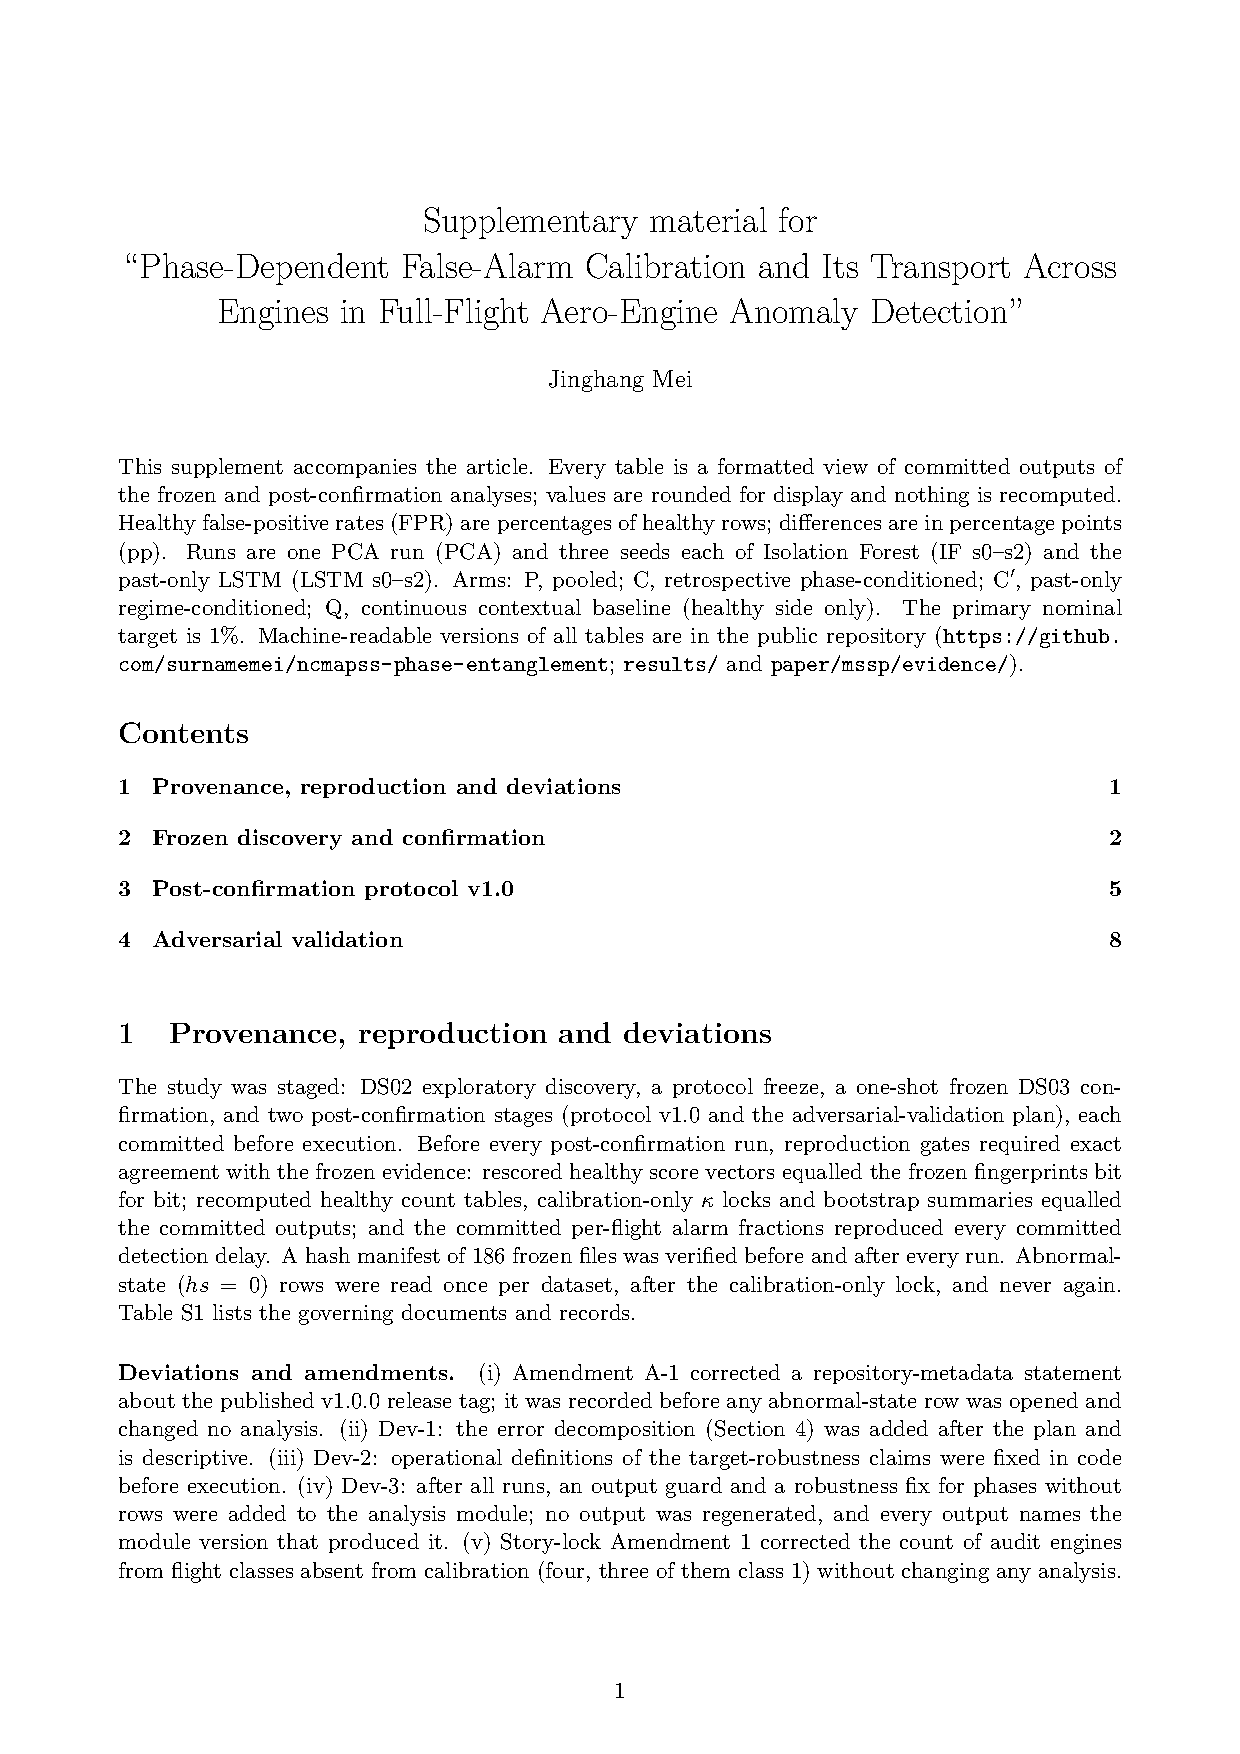
\includepdf[pages=-]{../../mssp/supplement/supplement.pdf}
\end{document}
